\documentclass[uplatex,dvipdfmx]{jsarticle}
\usepackage{amsmath,amssymb,amssymb}
\usepackage{bm}
\usepackage{mathtools}
\usepackage{ascmac}
\usepackage{mathrsfs}
\usepackage{physics}
\usepackage{here}
\usepackage{url}
\usepackage{tikz-cd}
\usepackage[top=25truemm,bottom=30truemm,left=20truemm,right=20truemm]{geometry}
\usepackage{xcolor}
\usepackage{titlesec}
% 文字サイズを大きくする設定
\titleformat{\section}{\huge\bfseries}{\thesection}{1em}{}
\titleformat{\subsection}{\Large\bfseries}{\thesubsection}{1em}{}
\titleformat{\subsubsection}{\Large\bfseries}{\thesubsubsection}{1em}{}
\usepackage{tcolorbox}
\tcbuselibrary{breakable, skins, theorems}
\usepackage[dvipdfmx]{hyperref}
\usepackage{pxjahyper}
\usepackage{bookmark}
\setcounter{tocdepth}{3}
\usepackage[]{tcolorbox}
\usepackage{hyperref}
% プリアンブルに追加
\newtcolorbox{myprop}[2][]{%
    enhanced,
    colframe = blue!70!black,
    colback = white,
    title = Proposition~#2,
    fonttitle = \bfseries,
    breakable = true,
    coltitle = black,
    attach boxed title to top left = {xshift=5mm, yshift=-3mm}, 
    boxed title style = {colframe = blue!70!black, colback = white},
    top = 4mm,
    #1 % 追加のオプション（あれば）
}
\newtcolorbox{mycor}[2][]{%
    enhanced,
    colframe = blue!50!red,
    colback = white,
    title = Corollary~#2,
    fonttitle = \bfseries,
    breakable = true,
    coltitle = black,
    attach boxed title to top left = {xshift=5mm, yshift=-3mm}, 
    boxed title style = {colframe = blue!50!red, colback = white},
    top = 4mm,
    #1 % 追加のオプション（あれば）
}
\newtcolorbox{mythm}[2][]{%
    enhanced,
    colframe = red!80!black,
    colback = white,
    title = Theorem~#2,
    fonttitle = \bfseries,
    breakable = true,
    coltitle = black,
    attach boxed title to top left = {xshift=5mm, yshift=-3mm}, 
    boxed title style = {colframe = red!80!black, colback = white},
    top = 4mm,
    #1 % 追加のオプション（あれば）
}

\newtcolorbox{mydef}[2][]{%
    enhanced,
    colframe = green!35!black,
    colback = white,
    title = Definition~#2,
    fonttitle = \bfseries,
    breakable = true,
    coltitle = black,
    attach boxed title to top left = {xshift=5mm, yshift=-3mm}, 
    boxed title style = {colframe = green!35!black, colback = white},
    top = 4mm,
    #1 % 追加のオプション（あれば）
}

\newtcolorbox{mylemma}[2][]{%
    enhanced,
    colframe = blue!70!black,
    colback = white,
    title = Lemma~#2,
    fonttitle = \bfseries,
    breakable = true,
    coltitle = black,
    attach boxed title to top left = {xshift=5mm, yshift=-3mm}, 
    boxed title style = {colframe = blue!70!black, colback = white},
    top = 4mm,
    #1 % 追加のオプション（あれば）
}
\newtcolorbox{myex}[2][]{%
    enhanced,
    colframe = green!0!black,
    colback = white,
    title = Example~#2,
    fonttitle = \bfseries,
    breakable = true,
    coltitle = black,
    attach boxed title to top left = {xshift=5mm, yshift=-3mm}, 
    boxed title style = {colframe = green!0!black, colback = white},
    top = 4mm,
    #1 % 追加のオプション（あれば）
}
\newtcolorbox{myexercise}[2][]{%
    enhanced,
    colframe = green!40!blue,
    colback = white,
    title = Exercise~#2,
    fonttitle = \bfseries,
    breakable = true,
    coltitle = black,
    attach boxed title to top left = {xshift=5mm, yshift=-3mm}, 
    boxed title style = {colframe = green!40!blue, colback = white},
    top = 4mm,
    #1 % 追加のオプション（あれば）
}
% カスタム証明環境の定義

% カスタム証明環境の定義
\newtcolorbox{myproof}{
    empty, 
    breakable, 
    left=8mm, % 本文と左線の距離
    right=2mm,
    top=4mm,  % 見出し（線）からのテキストの距離
    bottom=4mm,
    fonttitle=\sffamily, 
    coltitle=black,
    title={proof}, 
    % --- タイトルの配置設定 ---
    attach boxed title to top left={xshift=0mm, yshift=0mm}, 
    boxed title style={
        empty, 
        size=minimal, 
        % タイトルの下に横線を引く（長さ10mm）
        underlay={
            \draw[line width=0.6pt] (-1mm,0) -- (9mm,0);
        }
    },
    underlay={
        % 1. まっすぐな垂直線（タイトルの少し左から開始）
        \draw[line width=0.6pt] 
            ([xshift=1mm, yshift=-1.5pt]title.south west) coordinate (A) 
            -- (A |- frame.south west) coordinate (B);
        % 2. L字の底（右へ5mm）
        \draw[line width=0.6pt] 
            (B) -- ++(5mm,0mm);
    }
}

\begin{document}
\color{white}A\color{black}\\
\begin{center}
  {\huge Lie代数と表現論ノート}
\end{center}
\color{white}A\color{black}
\begin{center}
  {\Large J.E. Humphreys~~~~~~~~Introduction to Lie Algebras and Representation Theory}
\end{center}
\color{white}A\color{black}\\\\
Humphreysの行間埋めノートです~~~~~~~~~~~~~~~~~~~~~~~~~~~~~~~~~~~~~~~~~~~~~~~~~~更新日~~~~~~2026/05/03
\\\\
\hypertarget{toc}{}\tableofcontents
\newpage

\section{Chapter I ~~ BASIC CONCEPTS}
\subsection{Definitions and first examples}
\subsubsection{The notion of Lie algebra}

\begin{mydef}{1.1~~~Lie代数}
    体$\mathbb{F}$上のベクトル空間$L$で
    \begin{equation*}
        [~,~]:L\times L\to L~~~~~(x,y)\mapsto [x,y]
    \end{equation*}
    という\textbf{ブラケット(btaket)}が定義され,~次の性質\\
    (L1)$[~,~]$が\textbf{双線形写像}\\
    つまり,~$\forall x,y,z\in L~~,\forall\lambda_i\in \mathbb{F}$~に対し
    \begin{equation*}
    \begin{split}
        [\lambda_1 x+\lambda_2 y,z] = \lambda_1[x,z]+\lambda_2 [y,z]\\
        [x,\lambda_1y+\lambda_2z]=\lambda_1[x,y]+\lambda_2[x,z]
    \end{split}
    \end{equation*}
    が成立する.\\
    (L2)$\forall x\in L$~に対し
    \begin{equation*}
        [x,x]=0
    \end{equation*}
    が成立する.\\
    (L3)$\forall x,y,z\in L$~に対して\textbf{Jacobi恒等式}
    \begin{equation*}
        [x,[y,z]]+[y,[z,x]]+[z,[x,y]]=0
    \end{equation*}
    が成立する.\\
    を満たす$(L,[,])$を\textbf{Lie代数}という.
\end{mydef}
(L1)(L2)から
\begin{equation*}
    [x+y,x+y]=[x,x+y]+[y,x+y]=[x,y]+[y,x]=0
\end{equation*}
が成立するので,~任意の$\forall x,y\in L $に対してLie braketは\textbf{反可換}
\begin{equation*}
    [x,y]=-[y,x]
\end{equation*}
であることが分かる.~また,~\textbf{(L2)を忘れ},~反可換性と双線形性を仮定することで
\begin{equation*}
    [x,x]=-[x,x]\Leftrightarrow[x,x]=0
\end{equation*}
が言える.~これは(L2)そのものなので,~\textbf{反可換性と(L2)は同値}であることが言える.
\newpage
Lie代数の例として以下のようなものがある.
\begin{myex}{1.1~~~Lie代数の例}
    (1)~$\mathbb{R}^3$と外積~$(\mathbb{R}^3,\times)$\\
    (2)~一般線形Lie代数~$\mathfrak{gl}(V)=(\text{End}~V,[~,~])$\\
    (3)~特殊線形Lie代数~$\mathfrak{sl}(V)$\\
    (4)~symplectic Lie代数~$\mathfrak{sp}(V)$\\
    (5)~直交代数~$\mathfrak{o}(V)$\\
    (6)~ベクトル場(多様体論)~$(\mathfrak{X}(M),[~,~])$~~特に,~Lie群の原点$e$での接空間$T_eG$\\
    (7)~相空間上の関数全体とpoisson括弧(解析力学)~$(C^\infty(TQ^*),\{~,~\})$
\end{myex}
\begin{myproof}
(1)~\textbf{外積}\\
$\forall\bm{x},\bm{y},\bm{z}\in \mathbb{R}^3$に対して,~外積$\times$は明らかに双線形性を満たし,~
\begin{equation*}
    \bm{x}\times\bm{x}=\bm{0}
\end{equation*}
であり,~\textbf{ベクトル3重積(vector triple product)}
\begin{equation*}
    (\bm{x}\times(\bm{y}\times \bm{z}))+(\bm{y}\times(\bm{z}\times \bm{x}))+(\bm{z}\times(\bm{x}\times \bm{y}))=\bm{0}
\end{equation*}
を満たす.\\\\
(2)~\textbf{一般線形Lie代数}\\
交換子$[~,~]:\text{End}~V\times \text{End}~V\to \text{End}~V$~を
\begin{equation*}
    [f,g]=f\circ g-g\circ f = fg-gf
\end{equation*}
で定義する.~これは一般に非可換である.\\
このとき,~明らかに双線形性と$[f,f]=0$を満たし
\begin{equation*}
    [f,[g,h]]+[g,[h,f]]+[h,[f,g]]=fgh-ghf-fhg+hgf+ghf-hfg-gfh+fhg+hfg-fgh-hgf+gfh=0
\end{equation*}
を満たすので,~これはLie代数である.\\
また,~$\text{End}~V$に交換子がついたこのLie代数を一般線形代数と呼び,~$\mathfrak{gl}(V)$で表す.\\
また,~$V$が有限次元ベクトル空間の場合では基底をあらわに書けるので,~線形変換を考えると
\begin{equation*}
    \text{End}~V \simeq M(n,\mathbb{F})
\end{equation*}
となることが分かる.~ここで$\dim V=n$~とした.\\\\
(3)から(5)は省略する.~線形Lie群のときに証明する.\\\\
(6)~\textbf{ベクトル場}\\
任意の$\forall X,Y\in \mathfrak{X}(M)$に対してbraketを
\begin{equation*}
    [X,Y]f = X(Yf)-Y(Xf)~~~~~\forall f\in C^\infty(M)
\end{equation*}
で定義する.~ここで一般に~$XY\notin \mathfrak{X}(M)$であるが,~$[X,Y]\in \mathfrak{X}(M)$となることに注意する必要がある.\\
実際,~座標近傍を$(U,x_1,\cdots x_n)$として$[X,Y]$の局所座標表示を考えると$X|_U = \sum a_i\frac{\partial}{\partial x_i},~Y|_U = \sum b_i\frac{\partial}{\partial x_i}$として
\begin{equation*}
    [X,Y]|_U = \sum_i\sum_j \left( a_j\frac{\partial b_j}{\partial x_j}-b_j\frac{\partial a_j}{\partial x_j} \right)\left( \frac{\partial}{\partial x_i} \right)_U\in \mathfrak{X}(U)
\end{equation*}
となるので,~braketはベクトル場で閉じること
\begin{equation*}
    [~,~]:\mathfrak{X}(M)\times \mathfrak{X}(M)\to \mathfrak{X}(M)~~~~~~(X,Y)\mapsto[X,Y]
\end{equation*}が確かめられる.\\
また,~定義より双線形性が成り立ち,~\textbf{jacobi恒等式}
\begin{equation*}
    [X,[Y,Z]]+[Y,[Z,X]]+[Z,[X,Y]]=0
\end{equation*}
が成立する.~この$0\in \mathfrak{X}(M)$は$M$の各点$p$にゼロベクトルを対応させるベクトル場である.\\
Jacodi恒等式の証明は(2)と同じのため省略する.\\\\
(7)~\textbf{相空間上の関数全体とPoisson括弧}\\
ポアソン括弧(Poisson braket)の定義にはハミルトンベクトル場$X_g,Y_f$とsymplectic 2形式$\Omega$のsymplectic内積
\begin{equation*}
    \{f,g\}_p = \ev{\Omega|X_g,Y_f} = \sum_{i}\left( \frac{\partial f}{\partial q^i} \frac{\partial g}{\partial p_i}-\frac{\partial f}{\partial p_i}\frac{\partial g}{\partial q^i}\right)
\end{equation*}
で定義できるが,~一般的な解析力学ではsymplectic内積の結果のみを用いて
\begin{equation*}
    \{f,g\}_p =  \sum_{i}\left( \frac{\partial f}{\partial q^i} \frac{\partial g}{\partial p_i}-\frac{\partial f}{\partial p_i}\frac{\partial g}{\partial q^i}\right)
\end{equation*}
でPoisson括弧$\{,\}:C^\infty (TQ^*)\times C^\infty(TQ^*)\to C^\infty (TQ^*)$を定義する.\\
ここで,~$C^\infty (TQ^*)$は相空間上の関数全体の集合とする.\\
Poisson括弧は明らかに双線形性があり,~$\{f,f\}_p = 0$~となる.\\
また,~これも任意の$f,g,h\in C^\infty(TQ^*)$~に対してJacobi恒等式
\begin{equation*}
    \{f,\{g,h\}\}+\{g,\{h,f\}\}+\{h,\{f,g\}\}=0
\end{equation*}
が成り立つ.~証明は計算するだけなので省略する.
\end{myproof}
\begin{mydef}{1.2~~~Lie代数の同型}
    $L,L'$を体$\mathbb{F}$上のLie代数とする.\\
    ベクトル空間上の\textbf{同型}$\phi:L\to L'$~があり,~任意の$\forall x,y\in L$に対して
    \begin{equation*}
        \phi([x,y])=[\phi(x),\phi(y)]
    \end{equation*}
    が成立するとき,~Lie代数$L,L'$は\textbf{同型}といい,~$\phi$をLie代数の同型ともいう.
\end{mydef}
\newpage
\subsubsection{Linear Lie algebras}
\begin{mydef}{1.3~~~部分Lie代数}
    $\mathbb{F}$上のLie代数$L$の部分集合$K\subset L$が\textbf{部分Lie代数}であるとは,~任意の$\forall a,b\in K$~に対して
    \begin{equation*}
        [a,b]\in K\subset L
    \end{equation*}
    が成り立つことである.
\end{mydef}
このbraketはLie代数$L$に付随するものである.~次に\textbf{線形Lie代数}と呼ばれる$\mathfrak{gl}(V)$の部分Lie代数を考える.

\begin{mydef}{1.4~~~線形Lie代数}
    線形Lie代数とは,~一般線形代数$\mathfrak{gl}(V)$の部分Lie代数である.
\end{mydef}
$\mathfrak{gl}(V)$の部分Lie代数なので,~braketは交換子$[f,g]=fg-gf$~で定義される.\\
線形Lie代数には以下のようなものがある.

\begin{myex}{1.4~~~線形Lie代数の例}
    (1)特殊線形Lie代数~~$\mathfrak{sl}(V)=\{X\in \mathfrak{sl}(V)~|~\Tr(X)=0\}$\\
    (2)直交Lie代数 ~~$\mathfrak{so}(V)=\{X\in \mathfrak{so}(V) ~|~X^T = -X\}$\\
    (3)狭義上三角行列 ~~$\mathfrak{t}(n,\mathbb{F})= \{ X\in \mathfrak{t}(n,\mathbb{F})~|~X\in \text{狭義上三角行列全体の集合}\}$\\
    (4)上三角行列 ~~$\mathfrak{n}(n,\mathbb{F})= \{ X\in \mathfrak{n}(n,\mathbb{F})~|~X\in \text{上三角行列全体の集合}\}$\\
    (5)対角行列 ~~$\mathfrak{d}(n,\mathbb{F})= \{ X\in \mathfrak{d}(n,\mathbb{F})~|~X\in \text{対角全体の集合}\}$
\end{myex}
\begin{myproof}
(1)$\forall X,Y\in \mathfrak{sl}(V)$に対して
\begin{equation*}
    \Tr[X,Y]=\Tr(XY-YX) = \Tr(XY)-\Tr(YX)=0
\end{equation*}
より,~$[X,Y]\in \mathfrak{sl}(V)$~よって,~$\mathfrak{sl}(V)$~は線形Lie代数である.\\\\
(2)$\forall X,Y\in \mathfrak{so}(V)$に対して
\begin{equation*}
    ([X,Y])^T = (XY-YX)^T = Y^TX^T -X^TY^Y =YX-XY= -[X,Y]
\end{equation*}
より,~$[X,Y]\in \mathfrak{so}(V)$~よって,~$\mathfrak{so}(V)$~は線形Lie代数である.\\\\
(3)$\forall X,Y\in \mathfrak{t}(n,\mathbb{F})$に対して
\begin{equation*}
    [X,Y]=XY-YX\in \mathfrak{n}(n,\mathbb{F})\subset\mathfrak{t}(n,\mathbb{F})
\end{equation*}
より,~$[X,Y]\in \mathfrak{t}(n,\mathbb{F})$~よって,~$\mathfrak{t}(n,\mathbb{F})$~は線形Lie代数である.\\\\
(4)$\forall X,Y\in \mathfrak{n}(n,\mathbb{F})$に対して
\begin{equation*}
    [X,Y]=XY-YX\in \mathfrak{n}(n,\mathbb{F})
\end{equation*}
より,~$[X,Y]\in \mathfrak{n}(n,\mathbb{F})$~よって,~$\mathfrak{n}(n,\mathbb{F})$~は線形Lie代数である.\\\\
(5)$\forall X,Y\in \mathfrak{d}(n,\mathbb{F})$に対して
\begin{equation*}
    [X,Y]=XY-YX=0\in \mathfrak{d}(n,\mathbb{F})
\end{equation*}
より,~$[X,Y]\in \mathfrak{d}(n,\mathbb{F})$~よって,~$\mathfrak{d}(n,\mathbb{F})$~は線形Lie代数である.
\end{myproof}
\newpage
\subsubsection{Lie algebras of derivations}
\begin{mydef}{1.5~~~$\mathbb{F}$-代数}
    $\mathfrak{U}$を$\mathbb{F}$上ベクトル空間とする.~このとき,~二項演算
    \begin{equation*}
        \star:\mathfrak{U}\times \mathfrak{U}\to \mathfrak{U}
    \end{equation*}
    が定義されていて,~$\forall x,y,z\in \mathfrak{U},~\forall\lambda_1,\lambda_2 \in \mathbb{F}$~に対して\textbf{双線形性}
    \begin{equation*}
        x\star(\lambda_1 y + \lambda_2 z)=\lambda_1x\star y + \lambda_2 x\star z
    \end{equation*}
    \begin{equation*}
        (\lambda_1 y + \lambda_2 z)\star x=\lambda_1y\star x + \lambda_2 z\star x
    \end{equation*}
    を満たすとき,~$\mathfrak{U}$~を\textbf{$\mathbb{F}$-代数}という.
\end{mydef}
Lie代数$L$にも双線形性を持つ二項演算$L\times L\to L$としてbraketがあるので,~\textbf{Lie代数も$\mathbb{F}$-代数}である.

\begin{mydef}{1.6~~~$\mathbb{F}$-代数における微分}
    $\mathbb{F}$代数$\mathfrak{U}$における\textbf{微分}とは,~線形写像$\delta:\mathfrak{U}\to \mathfrak{U}$~で$\forall a,b\in \mathfrak{U}~$に対して\\
    \textbf{Leibniz則}
    \begin{equation*}
        \delta(a\star b)=\delta(a)\star b+a\star \delta(b)
    \end{equation*}
    を満たすものである.\\
    また,~$\mathfrak{U}$の微分全体を$\text{Der}~\mathfrak{U}$~と呼び,~これは$\text{End}~\mathfrak{U}$の部分ベクトル空間である.
\end{mydef}
より強く,~$\text{Der}~\mathfrak{U}$は\textbf{線形Lie代数},~つまり$\mathfrak{gl}(\mathfrak{U})$の部分Lie代数と言える.\\
\begin{myproof}
$\forall d,\delta \in \text{Der}\mathfrak{U}~,\forall a,b\in \mathfrak{U}$~に対して
\begin{equation*}
    \begin{split}
        [d,\delta](a\star b)&=d\delta (a\star b)-\delta d(a\star b)\\
        &=d\left( \delta(a)\star b +a\star \delta (b)  \right)-\delta \left( d(a)\star b +a\star d (b)  \right)\\
        &=(d\delta -\delta d)(a)\star b+a\star(d\delta -\delta d)(b)\\
        &=[d,\delta ](a)\star b+a\star [d,\delta ](b)
    \end{split}
\end{equation*}
が成り立つ.~よって,~$\text{Der}~\mathfrak{U}$は線形Lie代数であることが示された.
\end{myproof}
Lie代数としての$\text{Der}~\mathfrak{U}$を\textbf{微分代数}(derivation algebra)という.\\\\
\textbf{Example $\text{ad}~x$}\\
次に$\mathbb{F}$-代数をより狭くLie代数として微分代数$\text{Der}~L$を考える.~$\mathbb{F}$-代数の2項演算$\star$をbraket$[~,]~$として考える.~\\
ここで,~次のような線形写像はLie代数の種類によらず$\text{Der}~L$の元であると言える.\\
$x\in L$~を任意に固定して
\begin{equation*}
    \text{ad}~x :L\to L ~~~~~~y\mapsto[x,y]
\end{equation*}
という線形写像を考える.~このとき\textbf{Jacobi恒等式}から
\begin{equation*}
    \text{ad} ~x([y,z]) =[x,[y,z]]=[[x,y],z]+[y,[x.z]]=[\text{ad}~x(y),z]+[y,\text{ad}~x(z)]
\end{equation*}
が言えるので,~$\text{ad}~x\in \text{Der}~L$~となる.\\
つまり,~braket$[~,~]$はLie代数の条件である\textbf{Jacobi恒等式}考えることで本質的に\textbf{微分}と同じ役割を持てることが分かる.~$\text{ad}~x$~の形で書ける微分代数の元を\textbf{内部微分}といい,~そうでない元を\textbf{外部微分}という.\\\\
似たような話は代数以外にも表れる.\\\\
\textbf{Example 1~~~Lie微分(多様体論)}\\
$\varphi_t$をベクトル場$X$で生成されるフロー(flow)とする.\\
このとき,~ベクトル場の\textbf{Lie微分}を
\begin{equation*}
    \mathcal{L}_X Y=\lim_{t\to 0} \frac{(\varphi_{-t})_*Y -Y}{t}
\end{equation*}
で定義すると
\begin{equation*}
    \mathcal{L}_XY = [X,Y]
\end{equation*}
を満たすことが分かる.~(証明は松本多様体 $\S$17補足 を参照)\\
ベクトル場$\mathfrak{X}(M)$は交換子でLie代数を構成するので,~
\begin{equation*}
    \mathcal{L}_X([Y,Z])=[X,[Y,Z]]=[\mathcal{L}_XY,Z]+[Y,\mathcal{L}_X Z]
\end{equation*}
を満たすことが分かる.~これは$\text{ad}$を$\mathcal{L}$に変えた式であるが,~Lie微分の微分としての性質をbraketが保証しているとも言うことができるだろう.\\\\
\textbf{Example 2~~~Poisson 括弧(解析力学, 量子力学)}\\
簡単のため,~総空間上の関数は時間に陽に依存しないとする.
Poisson括弧も相空間(phase spase)上の関数全体をLie代数とすることが分かる.\\
この事実と微分代数の知識から,~Poisson括弧も微分としての役割を持つことが予測される.\\
実際,~Leibniz則
\begin{equation*}
    \{fg,h\}_p = f\{g,h\}_p+g\{f,h\}
\end{equation*}
を満たすことが計算により確かめられる.~Poisson括弧と微分の性質として,~正準力学の重要な方程式である
\begin{equation*}
    \frac{df}{dt}=\{f,H\}
\end{equation*}
がある.~この式は,~Poisson括弧が微分としての役割を持つことを保証しており,~さらに系の時間発展に対する物理量の\textbf{保存}を示唆していることが分かる.~実際,~この式はLie微分の式と本質的に同じことを言っており,~解析力学をsymplectic幾何学を用いて定式化する際にはHamiltonベクトル場によって生成されるフローを考え,~その軌道上で物理量の保存を議論することができる.~これはLie代数のノートなので詳しくは述べないが,~多様体論で以下のような補題がある.\\\\
\textbf{補題}\\
~~~$X,Y$を完備なベクトル場とする.\\
~~~$[X,Y]=0$であるための必要十分条件は,~$\forall t\in \mathbb
R$について$(\varphi_t)_*Y=Y$~が成り立つことである.\\\\\\
また,~正準量子化を通して量子力学に対しても同じようなことが言える.~(無限次元であるが)\\
Heisenbergの運動方程式
\begin{equation*}
    \frac{d \hat{\mathcal{O}}}{dt}=\frac{1}{i\hbar}[\hat{\mathcal{O}},\hat{H}]
\end{equation*}
ここに出現する交換子も
\begin{equation*}
    [\hat{A}, \hat{B}\hat{C}] = [\hat{A}, \hat{B}]\hat{C} + \hat{B}[\hat{A}, \hat{C}]
\end{equation*}
というLeibniz則を満たす.\\
この関係は量子力学の演算子の計算に対して以下のような応用が利く.
\begin{equation*}
    [A, B^n] = \sum_{k=0}^{n-1} B^k [A, B] B^{n-1-k}
\end{equation*}
特に,$[A,B]$が定数(c数)の場合は
\begin{equation*}
    [A, B^n] = n [A, B] B^{n-1}
\end{equation*}
が成り立つので,~演算子による展開を考えると
\begin{equation*}
    [A, f(B)] = [A, B] \frac{df}{dB}
\end{equation*}
が言える.~例えば
\begin{equation*}
    [\hat{x}, \sin(\hat{p})] = i\hbar \frac{\partial \sin({p})}{\partial p}=i\hbar \cos(\hat{p})
\end{equation*}
が成り立つ.
\newpage
\subsubsection{Abstract Lie algebras}
\subsection{Ideals and homomorphisms}
\subsubsection{Ideals}
\subsubsection{Homomorphisms and representations}
\subsubsection{Automorphisms}
\subsection{Solvable and nilpotent Lie algebras}
\subsubsection{Solvability}
後で書きます\newpage
\subsubsection{Nilpotency}
\begin{mydef}{3.2~~~冪零Lie代数}
    $L$をLie代数とする.~$L$に対して
    \begin{equation*}
        L^0 = L ~~~~L^1=[L,L]~~~~L^i=[L,L^{i-1}]
    \end{equation*}
    のような減少列
    \begin{equation*}
        L=L^0 \supset L^1 \supset L^2 \supset \cdots \supset L^i \supset \cdots
    \end{equation*}
    を定義する.~この減少列が\{0\}で止まるとき,~すなわち
    \begin{equation*}
        L^{N-1} \neq 0~~~~~~~  L^N=[L,L^{N-1}]=0
    \end{equation*}
    となる$N\in \mathbb{N}\setminus \{0\}$が存在するとき,~$L$を\textbf{冪零(Nilpotent)Lie代数}という.
\end{mydef}
注意:~$L$の微分列から定義される$L^{(i)}$と区別するために括弧()を付けないようにする.\\\\
また,~帰納的に考えることで
\begin{equation*}
    L^{(1)}=[L,L]=L^1~~~~~~~L^{(2)}=[L^1,L^1]\subset [L,L^1]
\end{equation*}
より
\begin{equation*}
    L^{(i)}=[L^{(i-1)},L^{(i-1)}]\subset [L,L^{i-1}]=[L.L^i]
\end{equation*}
が得られる.~また,~$L$がべき零Lie代数のとき,~定義から任意の$x\in L$に対して~ad $x$~がべき零となることが分かる.\\
この逆を言えるのが次節で証明する\textbf{Engelの定理}である.~これはLie代数のべき零性をadで特徴付けている.

\begin{myprop}{3.2~~~冪零Lie代数の性質}
    $L$をLie代数とする.~また$f:L\to K$をLie準同型とする.\\
    (a)$L$がべき零Lie代数ならば~$L$の任意の部分Lie代数$A$は冪零 Lie代数である.\\
    ~~~~また,~$\text{Im} f$もべき零Lie代数となる.\\
    (b)$L$がべき零Lie代数ならば,~任意の$L$のイデアル$I$に対して構成される商Lie代数$L/I$もべき零Lie代数となる.\\
    (c)$L/Z(L)$がべき零Lie代数ならば,~$L$もべき零Lie代数である.\\
    (d)$L$が非零のべき零Lie代数ならば,~$Z(L)\neq 0$である.
\end{myprop}
\begin{myproof}
(a)~
$L$のべき零性より,~$L^N=0$となる$N>0$が存在する.~また,~$A\subset L$なので,~$A$に関する減少列を考えることで帰納的に$A^i \subset L^i$となる.~よって,~$A^N=0$となる$N>0$は存在するので$A$もべき零Lie代数である.\\
$f$はLie準同型なので,
\begin{equation*}
    f(L^1)=f([L,L])=[\text{Im}f,\text{Im}f]=(\text{Im}f)^1
\end{equation*}
となる.~帰納的に考えると
\begin{equation*}
    f(L^i)= [\text{Im}f,f(L^{i-1})]=(\text{Im}f)^i
\end{equation*}
が言えるので,~$L$がべき零Lie代数ならば$(\text{Im}f)^N=0$となる$N>0$が存在する.\\
よって,~Im $f$はべき零Lie代数である.\\\\
(b)~射影$\pi : L\to L/A ~~~x\mapsto x+A$はLie準同型写像である.
実際,~$\forall x,y \in L~~~\forall a,b \in \mathbb{K}$に対して
\begin{equation*}
    \pi(ax+by)=ax+by+A = a(x+A)+b(y+A) = a\pi (x)+b\pi (y)
\end{equation*}
\begin{equation*}
    \pi ([x,y])=[x,y]+A = [x+A,y+A]=[\pi(x),\pi(y)]
\end{equation*}
が成立することが確かめられる.\\
よって,~(a)より$\text{Im}~\pi = L/A$はべき零Lie代数となる.\\\\
(c)~$L/Z(L)$のべき零性より,~$(L/Z(L))^N=0$となる$N>0$が存在する.\\
準同型な射影$\pi:L\to L/Z(L)$を考えると,~(a)より
\begin{equation*}
    (L/Z(L))^N =(\text{Im}~\pi)^N=\pi(L^N)=0
\end{equation*}
なので,~$L^N\subset Z(L)$である.~$L$の減少列を考えると$L^N$は中心に入るので
\begin{equation*}
    L^{N+1}=[L,L^N]=0
\end{equation*}
となる.よって,~$L$はべき零Lie代数となる.\\\\
(d)~$L$はべき零Lie代数なので,~$L^{N-1}\neq 0,~L^N=0$となるような$N>0$が存在する.~ここで,中心の定義より
\begin{equation*}
    L^N=[L,L^{N-1}]=0~~~~~~~~~L^{N-1}\subset Z(L)
\end{equation*}
となるので,~$Z(L)\neq 0$であることが示された.
\end{myproof}
\newpage
\subsubsection{Proof of Engel's Theorem}
Engelの定理を示す前にいくつかの重要な補題を示す.
\begin{mylemma}{3.3.1}
    $x\in \mathfrak{gl}(V)$がべき零ならば,~ad$x \in \mathfrak{gl}(\mathfrak{gl}(V))$もべき零である
\end{mylemma}
\begin{myproof}
べき零性より,~$x^N=0$となる$N\in \mathbb{N}\setminus\{0\}$が存在する.\\
$x$による左移動,~右移動を
\begin{equation*}
    \lambda_x : \mathfrak{gl}(V) \to \mathfrak{gl}(V) \quad (y \mapsto xy)
\end{equation*}
\begin{equation*}
    \rho_x : \mathfrak{gl}(V) \to \mathfrak{gl}(V) \quad (y \mapsto yx)
\end{equation*}
とする.\\
$(\lambda_x^N) y = x^N y, \quad (\rho_x^N) y = y x^N$ より,~$x$ のべきゼロ性から $\lambda_x, \rho_x$ もべき零.\\
また,~任意の$y \in \mathfrak{gl}(V)$ に対して $\text{ad}\,x(y) = [x, y] = (\lambda_x - \rho_x)(y)$~となるので
\begin{equation*}
    \begin{split}
        (\text{ad}\,x)^{2N} &= (\lambda_x - \rho_x)^{2N} \\ &= \sum_{k=0}^{2N} \binom{2N}{k} (\lambda_x)^k (-\rho_x)^{2N-k} 
    \end{split}
\end{equation*}
$\sum$ の第 $0 \sim N$ 項で $\rho_x$ のべき零性,~第 $N \sim 2N$ 項で $\lambda_x$ のべき零性が現れるので $(\text{ad}\,x)^{2N} = 0$ \\
よって,~$\text{ad}\,x \in \mathfrak{gl}(\mathfrak{gl}(V))$ はべき零である .~~$\square$\\
また,~$\rho_x,\lambda_x$のべき零性より$\text{ad}~x^{2N-1}=0$ともなれる.
\end{myproof}
\newpage
\begin{mythm}{3.3.2}
    $V\neq\{0\}$を有限次元ベクトル空間,~$\mathfrak{gl}(V)$の任意の部分Lie代数を$L$とする.\\
    このとき,~任意の$x\in L$がべき零ならば,~ある$v\in V \setminus\{0\}$が存在して,~任意の$x\in L$に対して$x(v)=0$を満たす.
\end{mythm}
\textbf{step of proof}\\
$\dim L=0$のときは明らか.~$\dim V $に関する数学的帰納法で示す.\\
step1:\\
$L$の部分Lie代数を$K\subsetneq L$とする.~$\dim L\leq m-1$でTheorem~3.3.2が成立すると\textbf{仮定}すると,~$K \subsetneq N_L(K)$となることを示す.\\
step2:\\
$K$を極大部分Lie代数とすると,~$N_L(K)=L$となり,~$\dim L - \dim K =1$であることを示す.\\
step3:\\
$W=\{v\in V ~|~\forall y \in K ,~y(v)=0~\}$がstep2からnonzeroな$V$の部分ベクトル空間であることを示し,~その元を用いて$v$を構成すると題意を満たすようなものの存在性を示すことができる.\\\\
\begin{myproof}
$\cdot$~$\dim V=0$のとき~$L=\{0\}$より~$x(v)=0$となる$v$は必ず存在.\\
$\cdot$~$\dim V=1$のとき~$L=\mathbb{F}x$となる$x\in L$が存在してべき零性より$x^{N-1} \neq 0 ~, x^N =0$となる$N\in \mathbb{N}\setminus \{0\}$が存在.\\
次に$x^{N-1}(w)\neq 0$となる$w\in V$を取る.~取れないならば$x^{N-1}(w)=0$となる$w\in V$は存在するので証明が終わる.\\
$v=x^{N-1}(w)$とすれば$x(v)=0$となる$x\in V$は$w$から必ず構成できる.~これは任意の$x\in L$に対して言えるので示された.\\
$\cdot $~$\dim L \leq m-1$のとき,~命題が真であるとする.\\
$L$の部分Lie代数$K \subsetneq L$を任意に1つ取る.\\
$\text{ad}:L\to \mathfrak{gl}(L)$の制限$\text{ad}|_K:K\to \mathfrak{gl}(L)$の像$\text{Im~ad} $の任意の元$\text{ad}~x\in \text{Im~ad}$はLemma~3.3.1~よりべき零である.\\
$L,K$のLie代数としての構造を忘れて$\mathbb{F}$上ベクトル空間としたとき,~$L/K$を作れる.~ここで任意の$x\in L$に対して
\begin{equation*}
    \text{Ad}|_K(x):L/K\to L/L ~~~~y+K \mapsto\text{ad}(x)(y)+K
\end{equation*}
がwell-definedな線形写像であることを示す.~$\text{ad}$の線形性と$K$の部分Lie代数の定義より
\begin{equation*}
    \begin{split}
        \text{Ad}|_K(x)(y'+K)&=\text{ad}(x)(y')+K\\
        &=\text{ad}(x)(y)+\text{ad}(x)(y'-y)+K\\
        &=\text{ad}(x)(y)+[x,y'-y]+K\\
        &=\text{Ad}|_K(x)(y+K)
    \end{split}
\end{equation*}
より,~$\text{Ad}|_K(x)$はwell-definedであり,~$\text{ad}$の線形性から線形写像である.\\
また,~$\text{ad}$の準同型性より,~
\begin{equation*}
    \text{Ad}|_K:K\to \mathfrak{gl}(L/K)~~~~x\mapsto \text{Ad}|_K(x)
\end{equation*}
もwell-definedなLie代数の準同型である.~Lemma~3.3.1~より$\text{Ad}|_K(x)$はべき零であり$\text{Im Ad}|_K $は$\mathfrak{gl}(L/K)$の部分Lie代数であることが分かる.\\
帰納法の仮定を$V\to L/K~,~L\to \text{Im Ad}|_K$とすると,~$\dim \text{Im Ad}|_K \leq \dim(L/K)<\dim L$より,~ある$v+K \in L/K \setminus\{0+K\}$が存在して,~任意の$\text{Ad}|_K(x)\in \text{Im Ad}|_K$に対して$\text{Ad}|_K(x)(v+K)=0+K$が成り立つということである.これを言い換えると,
\begin{equation*}
    \text{Ad}|_K(x)(v+K)=\text{ad}(x)(v)+K=0+K
\end{equation*}
より,~$\text{ad}(x)(v)=[x,v]\in K$.~すなわち$v \in N_L(K)$であることを保証する.\\
また,~正規化代数$N_L(K)$の定義より$K\subset N_L(K)$となるので,~$K\subsetneq N_l(K),$~すなわち$K$が$N_L(K)$の真部分集合であることが分かる.\\
正規化代数の定義より,~$N_L(K)$は$K$をイデアルとする$L$の極大Lie部分代数である.\\
実際,~$K\subset N_L(K)$であり,~$\forall x\in N_L(K),~\forall y\in K$に対して~$[x,y]\in K$より$K$はイデアルとなる.~また,~$N_L(K)\subset J$として$J$のイデアルが$K$とすると,~$\forall x\in J,~\forall y\in K$に対して~$[x,y]\in K$~が成立.~しかし,~正規化代数の定義より,~$J\subset N_L(K)$となるので$N_L(K)=J$.~よって,~$N_L(K)$は$K$をイデアルとする極大部分Lie代数である.\\
ここで,~$K$を$K\subsetneq L$を満たす極大部分Lie代数とする.\\
$N_L(K)\subset L$であり,~$K\subsetneq N_L(K)$であるので$K$の極大性から$N_L(K)=L$であることが分かる.\\
よって,~$N_L(K)=L$は$K$をイデアルとするので商Lie代数$L/K$を定義できる.\\
次に,~射影$\pi:L\to L/K~~~~x\in x\mapsto x+K$~を考える.\\
$\dim (L/K)>1$と仮定すると,~$\dim P=1~,P\subset L/K$という部分Lie代数が構成できることを確かめる.\\
実際,~$\forall x_1,x_2 \in \pi^{-1}(P) ~,\forall \lambda_1,\lambda_2 \in \mathbb{F}$とすると
\begin{equation*}
    \pi(\lambda_1x_1+\lambda_2x_2)=\lambda_1x_1+K+\lambda_2 x_2 +K=\lambda_1(x_1+K)+\lambda_2(x_2+K)=\lambda_1\pi (x_1)+\lambda_2\pi (x_2)\in P
\end{equation*}
\begin{equation*}
    \pi([x_1,x_2])=[x_1,x_2]+K=[x_1+K,x_2+K]=[\pi(x_1),\pi(x_2)]=0+K \in P
\end{equation*}
より,~$P$は$L/K$の部分Lie代数であり,~$\pi^{-1}(P)$は$L$の部分Lie代数となる.\\
また,~任意の$\forall y \in K$に対して~$\pi(y)=\bar{0}\in P$であるので,~$K\subset \pi^{-1}(P)$となる.\\
$\dim P=1$なので,~$\bar{0}\neq p \in P$となる元$p\in P$がある.~$\pi(x)=p\neq 0$となる$x\in L$が存在するので,~$\pi^{-1}(p)\notin K$~であり,~$\pi^{-1}(P)\subset L$~となる.\\
次に,~$\bar{x}\in L/K \setminus P$~を満たす$\bar{x}$が存在することから,~$\pi(x)=\bar{x}\notin P,~x\notin \pi^{-1}(P)~.$が分かるので,~$K \subsetneq \pi^{-1}(P) \subsetneq L$~が示された.~しかし,~これは$K$の極大性に矛盾する.~よって,~$\dim (L/K)=\dim L -\dim K =1$~であることが分かるので,~$\forall z\in L\setminus K$とすると任意の$x\in L$はある$h\in K $とある$r\in \mathbb{F}$で$x = h+rz$と表される.\\
よって,~任意の$z\in L\setminus K$に対して$L=K+z\mathbb{F}$と表されることが分かる.\\
ここで,~$L$の部分ベクトル空間$W=\{ v\in V ~|~\forall y\in K,~y(v)=0 \}$~を考える.~$\dim K <\dim L$より帰納法の仮定を用いて~$W\neq \{0\}$であることが分かる.~$K$は$L$のイデアルなので$\forall z\in L\setminus K,~\forall y\in K,~\forall w\in W $に対して
\begin{equation*}
    yz(w)=zy(w)-[z,y](w) = z \cdot 0 -0  = 0
\end{equation*}
が成り立つので,~$\forall w \in W$に対して$z(w) \in W$~が成立する.~$z\in L $より,~$z^{N-1}(w)\neq 0,~z^N(w)=0$~となる$N\in \mathbb{N}\setminus \{0\}$~が存在.~$v= z^{N-1}(w)$~とすると,~任意の$\forall x\in L $に対して
\begin{equation*}
    x(v)=(h+rz)(z^{N-1}(w))=0+rz^N(w)=0
\end{equation*}
となるので$v\in V\setminus\{0\}$が存在して$\forall x\in L$に対して$x(v)=0$~となる.~よって題意は示された.~~$\square$
\end{myproof}
\newpage
\begin{mythm}{3.3.3~~~Engelの定理}
    $L$を有限次元Lie代数とする.このとき以下の2つの命題は同値である.\\
    (1)~$L$はべき零Lie代数\\
    (2)~任意の$x\in L$に対して$\text{ad}~x$がべき零
\end{mythm}
\begin{myproof}
$(\Leftarrow)$べき零Lie代数の定義より自明に成り立つ.\\
$(\Rightarrow)~\dim L$に関する帰納法を用いる.\\
$\dim L =0,1$のとき自明.\\
$\dim L \leq m-1$のとき,~$(\Rightarrow)$側の主張を仮定する.\\
$\dim L = m$のとき,~$\text{Im ad}\subset \mathfrak{gl}(L)$よりTheorem 3.3.2を用いると,~ある$v\in L\setminus\{0\}$が存在して任意の$\forall \text{ad}(x)\in \text{Im~ad}$~に対して$\text{ad}(x)(v)=[x,v]=0$~を満たすことが分かる.~つまり,~$v\in Z(L)$のため,~$L$の中心は非ゼロである.\\
$\dim(L/Z(L)) < \dim L = m$~に対して,~$[x]=x+Z(L)\in L/Z(L)$~となり,~$[x]$はべき零なので,~Lemma 3.3.1~より$\text{ad}[x]$もべき零になる.\\
帰納法の仮定より,~$L/Z(L)$はべき零Lie代数となる.~\\
Proposition 3.2 (c)より,~"$L/Z(L)$がべき零$\Rightarrow L$もべき零"~となるので,~$L$はべき零Lie代数となる.\\
これにより帰納法は回るので,~題意は示された.~~$\square$
\end{myproof}
\newpage
\begin{mydef}{3.3.4~~~ベクトル空間の旗と安定化}
    $V$をn次元$\mathbb{K}$上ベクトル空間とする.~$V$の\textbf{旗}(flag)とは,~部分ベクトル空間の増大列
    \begin{equation*}
        \{0\}=V_0 \subset V_1 \subset V_2 \subset \cdots \subset V_n=V
    \end{equation*}
    であって,~$0\leq i \leq n$に対して$\text{dim}V_i =i$が成立するようなものである.\\
    また,~$x\in \text{End}V$が$0\leq i \leq n$について$x(V_i)\subset V_i$を満たすならば,~$x$は旗を\textbf{安定化}する(stabilize)という.
\end{mydef}
\begin{myprop}{3.3.5~~~強い安定性と狭義上三角行列}
    $L$は$\mathfrak{gl}(V)$の部分Lie代数であり,~任意の$x\in L$に対して$x$はべき零であるとする.\\
    このとき,
    \begin{equation*}
        \{0\}=V_0 \subset V_1 \subset V_2 \subset \cdots \subset V_n=V
    \end{equation*}
    という旗が存在し,~任意の$x\in L$は$x(V_i)\subset V_{i-1}\subset V_i$を満たす.\\
    すなわち,~$V$の基底を適当にとると$L\subset \mathfrak{n}_n(\mathbb{K})$となる.
\end{myprop}
\begin{myproof}
補題3より,~ある$v \in V\setminus\{0\}$が存在し,~任意の$x\in L$に対して$x(v)=0$~となる.\\
その$v\in V\setminus\{0\}$ に対して,~$V_1 = \ev{v}_{\mathbb{K}}$とすると$V_1\subset \text{Ker}~ x$であるので,~商ベクトル空間$W=V/V_1$を構成する.\\
$W$への$L$の作用$\tau :L\to \mathfrak{gl}(W)~~x\mapsto \bar{x}$~は
\[
\begin{tikzcd}[row sep=large, column sep=large]
    V \arrow[r, "x"] \arrow[d, "P"'] & V \arrow[r, "P"] \arrow[dl, phantom, "\circlearrowright"] & V/V_1 \\
    V/V_1 \arrow[rru, "\bar{x}"'] & &
\end{tikzcd}
\]
を可換にするように定まり.~これは準同型定理より一意な構成であることが分かる.\\
任意の$x\in L $はべき零なので,~任意の$\bar{x}\in \mathfrak{gl}(W)$もべき零となる.\\
$\dim V$ に関する帰納法を用いる.~$\dim V = 0, 1$ のときは自明.\\
$\dim W = \dim V - 1$ に対して主張を仮定すると,~$\bar{x}$ はべき零なので
\[
\{0\} = W_0 \subset W_1 \subset \dots \subset W_{\dim V - 1} = W = V/V_1
\]
という旗（flag）が存在して,~$\bar{x}$ によって旗は安定化される.~
さらに強く,
\[
\bar{x} : W_i \to W_{i-1} \subset W_i
\]
も言える.~

ここで,~$V_i$ を以下のように定義する.~
\[
V_i \equiv
\begin{cases}
\pi^{-1}(W_{i-1}) & (i = 1, 2, \dots, \dim V) \\
0 & (i = 0)
\end{cases}
\]
ここで,~ $\pi : V \to V/V_1$ は自然な射影である.~これを用いると
\[
\begin{tikzcd}[column sep=0.3em, row sep=3em]
    % 上の行 (Wの旗)
    % 先頭に空欄セルを2つ入れて位置を調整
    & & \{0\} = W_0 \arrow[d, "\pi^{-1}"] & \;\subset\; & W_1 \arrow[d, "\pi^{-1}"] & \;\subset\; & W_2 \arrow[d, "\pi^{-1}"] & \;\subset \cdots \subset\; & W_{\dim V - 1} = W \arrow[d, "\pi^{-1}"] \\
    % 下の行 (Vの旗)
    \{0\} = V_0 & \;\subset\; & V_1 & \;\subset\; & V_2 & \;\subset\; & V_3 & \subset \cdots \subset & V_{\dim V} = V
\end{tikzcd}
\]
という旗が存在する.\\
$\bar{x}$ に関する帰納法の仮定を用いると,~任意の $v \in V_i$ に対して
\[
\pi(x(v)) = x(v) + V_1 = \bar{x}(v + V_1) \in W_{i-2}
\]
となるので$\pi^{-1}(W_{i-2}) = V_{i-1} \ni x(v)$~
より,$x : V_i \to V_{i-1} \subset V_i$~が成り立つ.\\
よって帰納法より題意は示された.\\\\\\
次に,~$L \subset \mathfrak{n}_n(K)$ となること,~すなわち $\forall x \in L \triangleleft \mathfrak{gl}(V)$ の行列表示を考える.~

$V_0 \subset V_1 \subset V_2 \subset \dots \subset V_n = V$ に沿って基底を選ぶ.~

\begin{itemize}
    \item $V_1$ の基底として $e_1$,~つまり $V_1 = \langle e_1 \rangle_K$
    \item $V_2$ の基底として $e_1, e_2$,~つまり $V_2 = \langle e_1, e_2 \rangle_K$
    \item これを続けて,~$V_i = \langle e_1, \dots, e_i \rangle_K$ となるように基底を選ぶ.~
\end{itemize}

$\forall x \in L \triangleleft \mathfrak{gl}(V)$ という線型変換は $x(V_i) \subset V_{i-1}$ を満たすことが示されているので,~$x(e_j) \in V_{j-1}$ より
\[
x(e_j) = \sum_{k=1}^{j-1} a_{kj} e_k
\]
となる.~$j=1 \text{ のとき } x(e_1) = 0, \quad j=2 \text{ のとき } x(e_2) = a_{12} e_1$\\
これ続けてを行列表示すると,~$v = \sum_{i=1}^n v_i e_i$ として,~$x(v) = \sum_{i=1}^n v_i \sum_{k=1}^{i-1} a_{ki} e_k$ より,~

\[
\underbrace{
\begin{pmatrix}
0 & a_{12} & a_{13} & \cdots & a_{1n} \\
  & 0      & a_{23} & \cdots & a_{2n} \\
  &        & \ddots & \ddots & \vdots \\
  &        &        & 0      & a_{n-1,n}      \\
0 &        &        &        & 0
\end{pmatrix}
}_{x}
\underbrace{
\begin{pmatrix}
v_1 \\
\vdots \\
\\
v_n
\end{pmatrix}
}_{v}
\]
となる.~よって,~$L \subset \mathfrak{n}_n(K)$ である.~

実際,~狭義上三角行列の任意の元はべき零であり,~
\[
v = \begin{pmatrix} c \\ 0 \\ \vdots \\ 0 \end{pmatrix} \quad (c \in K\setminus \{0\})
\]
という $v \neq 0$ のベクトルは,~任意の $A \in \mathfrak{n}_n(K)$ に対して $Av = 0$ となることが確かめれる.~よって題意は示された.
\end{myproof}
\newpage
\begin{mylemma}{3.3.6}
    $L$をべき零Lie代数,~$I$を$L$のイデアルとする.\\
    $I\neq \{0\}$ならば~$I \cap Z(L)\neq \{0\}$である.~特に$Z(L)\neq \{0\}$でもある.
\end{mylemma}
\begin{myproof}
$I$ は $L$ のイデアルなので,~定義より~$\forall x \in L,\; \forall i \in I$ に対して $\text{ad}(x)(i)=[x, i] \in I$ が成り立つ.~よって
\begin{equation*}
    \text{ad}_I:L\to \mathfrak{gl}(I) ~~~,~x\mapsto \text{ad}~x
\end{equation*}
となり,~$\text{ad}_I(L) \subset \mathfrak{gl}(I)$ と言える.\\
補題2より,~ある $i \in I \setminus \{0\}$ が存在して,~$\forall \mathrm{ad}\,x \in \text{ad}_I(L)$ に対して
\begin{equation*}
    \text{ad}_I(x)(i) = [x, i] = 0
\end{equation*}
を満たす.\\
中心 $Z(L)$ の定義より,~$i \in I \cap Z(L)$ のため $I \cap Z(L) \neq \{0\}$ である.\\
$I = Z(L)$ としたとき,~$Z(L) \cap Z(L) = Z(L) \neq \{0\}$ でもある.~よって題意は示された.
\end{myproof}
\newpage
\section{Chapter I\hspace{-1.2pt}I ~~Semisimple Lie Algebras}
\subsection{Theorems of Lie and Cartan}
\subsubsection{Lie's Theorem}
べき零Lie代数に対するEngelの定理の本質は,~任意のべき零なLie代数の元に対して共通の固有ベクトルが存在することだった.~次の定理も性質は似ているが,~体$\mathbb{F}$が必要な固有値を全て含むことを保証するために,~代数閉体であることと標数が0であることも必要とする.
\begin{mydef}{4.1.1~~~代数閉体と標数}
    $\mathbb{F}$を体とする.~任意の定数でない1変数多項式$f(x)\in F[x]$に対し$\alpha\in \mathbb{F}$があり$f(\alpha)=0$となるとき,~$\mathbb{F}$を\textbf{代数閉体}であるという,\\
    また,~自然な環準同型$\phi:\mathbb{Z}\to \mathbb{F}~~~n\mapsto n\cdot 1 \in \mathbb{F}$の$\text{Ker}~\phi$を考える.\\
    $\text{Ker}~\phi$は素イデアルなので,~$\text{Ker}~\phi = (0)$もしくは素数$p$があり$\text{Ker}~\phi=p\mathbb{Z}$となる.\\
    $\text{Ker}~\phi = (0)$のとき,~$\mathbb{F}$の標数$\text{char}~\mathbb{K}$を0,~$\text{Ker}~\phi=p\mathbb{Z}$のとき,~$\mathbb{F}$の標数${\text{char}}~\mathbb{K}$をpと定める.
\end{mydef}
例えば,~複素数体$\mathbb{C}$は代数閉体であり,~有理数体$\mathbb{Q}$の標数は0,~$\mathbb{F}_p$はpである.
\begin{mydef}{4.1.2~~~ウェイト空間(weight space)}
    $V$を有限次元$\mathbb{F}$上ベクトル空間として$\mathfrak{gl}(V)$の部分Lie代数$L$を考える.~$\rho:L\to \mathfrak{gl}(V)$を表現とすると,~$\lambda\in \text{Hom}_{\mathbb{K}}(L,\mathbb{K})$に対し
    \begin{equation*}
        V_\lambda =\{v\in V~|~\forall x\in L ~,~x(v)=\lambda(x)v~\}
    \end{equation*}
    とおく.~$V_\lambda\neq0$のとき,~$\lambda$を$L$上の\textbf{ウェイト(weight)}という.\\
    また,~$V_\lambda\neq0$を\textbf{ウェイト空間(weight space)}という.
\end{mydef}
\begin{mythm}{4.1.3}
    $V$を有限次元$\mathbb{F}$上ベクトル空間として,~$\mathfrak{gl}(V)$の部分Lie代数$L$が可解だとする.\\
    このとき,~$V\neq 0$ならば$V$には任意の$x\in L$に対する共通固有ベクトルが存在する.
\end{mythm}
Proof step\\
Theorem~3.3.2のようにdim$L$に関する帰納法で示す.\\
Step1,~まずdim $I$=dim$L-1$となるような$L$のイデアル$I$が存在することを示す.\\
Step2,~任意の$x\in I$に対して,
\begin{equation*}
    x(v)=\lambda(x)v
\end{equation*}
が満たされるような~$v\in V\setminus \{0\}$と$\lambda:I\to \mathbb{K}$が存在することを示す.\\
Step3,~$V_\lambda=\{ w\in V~|~x(w)=\lambda(x)v  ~~~\forall x\in I \}$が$L$不変.~すなわち任意の$x\in L$に対して$x(V_\lambda)\subset V_\lambda$であることを示す.\\
Step4,~$L=I+\mathbb{F}z$とかけ,~Step3より$z$は$V_\lambda$上の線形変換を定める.~体は代数閉体なので固有多項式の根は必ず体上に存在して,~固有値を$\alpha$に対応する$z$の固有ベクトルを$v_0\in V_\lambda$とすると,~この$v_0$が共通固有ベクトルとなるので題意を満たす.
\begin{tcolorbox}[enhanced,
    colframe = red!90!black,
    colback = white,
    title = Theorem~4.1.4~~~Lieの定理,
    fonttitle = \bfseries,
    breakable = true,
    coltitle = black,
    attach boxed title to top left = {xshift=5mm, yshift=-3mm}, 
    boxed title style = {colframe = red!90!black, colback = white},
    top = 4mm]
    $L$を$\mathfrak{gl}(V)$の可解な部分Lie代数とし,~$\dim V = n < \infty$ とする.~\\このとき,~任意の$x\in L $は$V$内のある旗を安定化させる.\\
    よって,~適当な$V$の基底を定めることで$L\in \mathfrak{t}_n(\mathbb{F})$となる.
\end{tcolorbox}
Proof\\
Theorem 4.1.3~と$\dim L$に関する帰納法を用いて示す
\begin{tcolorbox}[enhanced,
    colframe = red!90!black,
    colback = white,
    title = Theorem~4.1.5~~~Corollary A,
    fonttitle = \bfseries,
    breakable = true,
    coltitle = black,
    attach boxed title to top left = {xshift=5mm, yshift=-3mm}, 
    boxed title style = {colframe = red!90!black, colback = white},
    top = 4mm]
    $\phi :L\to \mathfrak{gl}(V)$を有限次元表現とする.~このとき$L$が可解なら$\text{Im}~\phi = \phi(L)$も可解なので,~$\phi(L)$も$V$内のある旗を安定化させる.
\end{tcolorbox}
Proof : Lieの定理から成立する.
\begin{tcolorbox}[enhanced,
    colframe = red!90!black,
    colback = white,
    title = Theorem~4.1.6~~~Corollary B,
    fonttitle = \bfseries,
    breakable = true,
    coltitle = black,
    attach boxed title to top left = {xshift=5mm, yshift=-3mm}, 
    boxed title style = {colframe = red!90!black, colback = white},
    top = 4mm]
    $L$を可解とする.\\
    このとき,~$L$ のイデアルの列 $0 = L_0 \subset L_1 \subset \dots \subset L_n = L$ で,~$\dim L_i = i$ となるものが存在する.
\end{tcolorbox}
Proof\\
ad:$L\to \mathfrak{gl}(L)$は有限次元表現であるので,~$\text{ad} ~L$は可解となる.\\
よって,~$L$内のある旗を安定化させる.
\begin{equation*}
    \{0\}=L_0\subset L_1\subset \cdots \subset L_n=L~~~~~s.t. ~\dim L_i =i
\end{equation*}
任意の$\text{ad}~x\in \text{ad} ~L$に対して,~$\text{ad}(x)(L_i)\subset L_i$が安定化の条件なので,~$0\leq i \leq n$に対して$L_i$は$L$のイデアルである.よって題意は示された.
\begin{tcolorbox}[enhanced,
    colframe = red!90!black,
    colback = white,
    title = Theorem~4.1.7~~~Corollary C,
    fonttitle = \bfseries,
    breakable = true,
    coltitle = black,
    attach boxed title to top left = {xshift=5mm, yshift=-3mm}, 
    boxed title style = {colframe = red!90!black, colback = white},
    top = 4mm]
    $L$を可解とする.\\
    このとき$x \in [L,L]$ ならば $\text{ad}_L~ x$ はべき零である.~特に,~$[L,L]$ はべき零である.
\end{tcolorbox}
\newpage
\subsubsection{Jordan-Chevalley decomposition}
以下,~体$\mathbb{F}$の標数を0とする.\\
任意の$x\in M_n(\mathbb{K})$~は線形変換でJordan標準形にでき,~Jordan標準形は対角行列とべき零行列の和に直すことができる.~この章では,~任意の$x\in \text{End}V$を一意な半単純とべき零行列の和に直す方法を考える.
\begin{mydef}{4.2.1}
    $x\in \text{End}V$~が~\textbf{半単純}(semi-simple)とは,~「$x$の$\mathbb{F}$上最小多項式の根がすべて違う」ようなもの.\\
    また,~$\mathbb{F}$が代数閉体のとき,~同値な言い換えとして「$x$が対角化可能」とも言える.
\end{mydef}
ここで,~2つの可換で半単純な$x,y\in \text{End}~V$~は同時対角化であることに気をつける.
\begin{mylemma}{4.2.1}
    $x,y$が可換で半単純なら,~$x\pm y$~も半単純
\end{mylemma}
\begin{myproof}
    $x,y$が可換な半単純なので同時対角化可能
    \begin{equation*}
        x\ket{n}=\lambda_x\ket{n}~~~~~~~~y\ket{n}=\lambda_y\ket{n}
    \end{equation*}
    よって,~$(x\pm y) \ket{n}=(\lambda_x+\lambda_y )\ket{n}$~より,~$x\pm y$~は対角化可能で半単純となる.
\end{myproof}
これは当たり前の話だが,~$W\subset V$~として制限したとき,~$x(W)\subset W$~を満たせば$x\in \text{End}~W$~で半単純となる.
\begin{myprop}{4.2.1}
    $V$を$\mathbb{K}$上ベクトル空間,~$x\in \text{Emd}~V~$とする.\\
    (a)~次の条件を満たす$x_s,~x_n\in \text{End}~V$~が\textbf{一意}に存在する.
    \begin{equation*}
        x=x_s+x_n~~~~~~~[x_s,x_n]=0
    \end{equation*}
    ここで,~$x_s$は半単純,~$x_n$~はべき零とする.\\
    (b)~以下のような性質を満たす定数項を持たない1変数多項式$p(T),~q(T)$~が存在する.
    \begin{equation*}
        x_s = p(x)~~~~~~x_n=q(x)
    \end{equation*}
    特に
    \begin{equation*}
        [x_s,x]=[x_n.x]=[x_s,x_n]=0
    \end{equation*}
    を満たす.\\
    (c)~$A\subset B\subset V$~とする.\\
    $x(B)\subset A~$ならば,~$x_s(B)\subset A$~かつ~$x_n(B)\subset A$~を満たす.
\end{myprop}
$x=x_x+x_n$~という$x$の一意な分解を\textbf{ジョルダン・シュバレー分解}~(Jordan-Chevalley-decomposition)~という.\\
$x_s,~x_n$~をそれぞれ半単純成分(semisimple part)~べき零成分(nilpotent part)~という.
\begin{myproof}
    (後で書きます...)
\end{myproof}
\begin{mylemma}{4.2.2}
    $x\in \text{End}~V$~のJordan分解が$x=x_s + x_n$~となるとき\\
    $\text{ad}~x=\text{ad}~x_s + \text{ad}~x_n$~も$\text{ad}~x\in \text{End(End~V)}$~のJordan分解となる.
\end{mylemma}
\begin{myproof}
    (後で書きます...)
\end{myproof}
\begin{mylemma}{4.2.3}
    $\mathfrak{U}$を有限次元$F$-代数とする.~このとき、$\mathfrak{U}$ の微分全体の集合 $\text{Der}~\mathfrak{U}$ は,~そのすべての元$x\in \text{Der } \mathfrak{U}$ の半単純成分$x_s$とべき零成分$x_n$を含んでいる.\\
    すなわち,~$x\in \text{Der}~\mathfrak{U}$~ならば~$x_s,~x_n\in \text{Der}~\mathfrak{U}$~ということ.
\end{mylemma}
\begin{myproof}
    (後で書きます...)
\end{myproof}
\newpage
\subsubsection{Cartan's Criterion}
前章より,~$[L,L]$~がべき零Lie代数ならば,~定義より$L$~が可解になることが分かる.~また,~Engelの定理によって,~Lie代数のべき零性をその元のadのべき零性で必要十分に言えることが示せた.~すなわち,~$[L,L]$~がべき零ということと,~任意の$x\in [L,L]$~に対して$\text{ad}~x$~がべき零であることは同値であることが言える.\\
この章ではLie代数の可解性を自己準同型のトレースを用いて特徴づける.
\begin{mylemma}{4.3.1}
    $A \subset B$ を $\mathfrak{gl}(V)$（$\dim V < \infty$）の2つの部分空間とする.\\
    $M = \{x \in \mathfrak{gl}(V) \mid [x, B] \subset A\}$ という集合$M$があり,~ある$x \in M$ が,~すべての $y \in M$ に対して $\text{Tr}(xy) = 0$ を満たすとする.~このとき,~$x$ はべき零である.
\end{mylemma}
\begin{myproof}
    (後で書きます...)
\end{myproof}
可解性の判定条件を述べる前に,~有用な恒等式を示す.
\begin{mylemma}{4.3.2}
    $x,y,z \in \text{End}~V$~とする.~このとき
    \begin{equation*}
        \text{Tr}([x, y]z) = \text{Tr}(x[y, z])
    \end{equation*}
    が成り立つ.
\end{mylemma}
\begin{myproof}
    \begin{equation*}
    \begin{split}
        \text{Tr}([x, y]z)&=\text{Tr}(xyz-yxz)\\
        &=\text{Tr}(xyz)-\text{Tr}(xzy)\\
        &=\text{Tr}(x[y,z])
    \end{split}
    \end{equation*}
    より示された.~これによって,~括弧積を隣に移せることが分かる.
\end{myproof}
\begin{mythm}{4.3.3~~~Cartan's Criterion)}
    $L$を有限次元ベクトル空間$V$の$\mathfrak{gl}(V)$の部分Lie代数とする.\\
    すべての $x \in [L, L]$ および $y \in L$ に対して $\text{Tr}(xy) = 0$ が成り立つならば,~$L$ は可解である.
\end{mythm}
\begin{myproof}
    Lemma~4.3.1~の$A$を$[L,L]$~$B$を$L$~とする.~このとき
    \begin{equation*}
        M=\{z\in \mathfrak{gl}(V)~|~[z,L] \subset [L,L]\}
    \end{equation*}
    となり,~明らかに$L\subset M$~を満たす.~$x,y,z\in L$~とすると
    \begin{equation*}
        \text{Tr}([x,y]z)=\text{Tr}(x[y,z])=\text{Tr}([y,z]x)
    \end{equation*}
    が成り立ち,~$[y,z]\in [L,L]$~なので,~定理の仮定が成り立つならば$\text{Tr}([x,y]z)=0$~となる.\\
    Lemma~4.3.1~より,~任意の$w\in [L,L]\subset L\subset M$は任意の$z\in L\subset M$に対して~$\text{Tr}(wz)=0$~を満たすので,~任意の$z\in [L,L]$はべき零である.\\
    また,~$w$がべき零なら$\text{ad}~w$も前章の補題よりべき零であり,~Engelの定理より$[L,L]$がべき零Lie代数となる.~可解の定義より,~$L$が可解Lie代数となるので,~定理は示された.
\end{myproof}
\begin{mycor}{4.3.4}
    $L$をLie代数とする.~$\forall x\in [L,L],~\forall y\in L$~に対して$\text{Tr}(\text{ad}x~\text{ad}y)=0$~が成立するならば,~$L$は可解Lie代数.
\end{mycor}
\begin{myproof}
    $\forall \text{ad}~x\in\text{ad}([L, L]) = [\text{ad } L, \text{ad } L],~\forall y\in \text{ad}~L$~に対してCartan Criterion~を適用すると~$\text{ad}~L$~が可解Lie代数となる.~準同型定理より
    \begin{equation*}
        \text{ad}~L\simeq L/Z(L)
    \end{equation*}
    となり,~$Z(L)$~も可解なので,~前章prop3.1より$L$も可解となる.
\end{myproof}
\newpage
\subsection{Killing form}
\subsubsection{Criterion for semisimplicity}
\begin{mydef}{5.1.1}
    $x,y\in L$~に対して
    \begin{equation*}
        \kappa(x,y)\coloneqq \text{Tr}(\text{ad}~x,\text{ad}~y)
    \end{equation*}
    $\kappa$が$L$上双線形で対称のとき,~$K$は\textbf{Killing 形式}(Killing form)~とよばれる.
\end{mydef}
\textbf{Killing 形式の結合性}\\
\begin{equation*}
    \kappa([x, y], z) = \kappa(x, [y, z])
\end{equation*}
\begin{myproof}
    \begin{equation*}
        \begin{split}
            \kappa([x, y], z) &=\text{Tr}(\text{ad }[x, y],\text{ad } z)\\
            &=\text{Tr}([\text{ad }x, \text{ad }y],\text{ad } z)\\
            &=\text{Tr}(\text{ad }x, [\text{ad }y,\text{ad } z])\\
            &=\text{Tr}(\text{ad }x, \text{ad }[y,z])\\
            &=\kappa(x, [y, z])
        \end{split}
    \end{equation*}
    より示された.
\end{myproof}
\begin{mylemma}{5.1.2}
    $I$ を $L$ のイデアルとする.~$\kappa$ を $L$ のKilling形式,~$\kappa_I$ を$I$ のKilling形式とすると、$\kappa_I = \kappa|_{I \times I}$ である.
\end{mylemma}
\begin{myproof}
    線形代数より,~$W$ が（有限次元）ベクトル空間 $V$ の部分空間であり,~$\phi\in \text{Hom}(V,W)$~のとき,~$\text{Tr} \phi = \text{Tr}(\phi|_W)$ である.\\
    $x,y\in I$~とすると,~任意の$z\in L$に対してイデアルの定義より$\text{ad}~x,\text{ad}~y(z)\in I$~となるので,~
    \begin{equation*}
        \begin{split}
            \kappa _I(x,y)&= \text{Tr}(\text{ad}_I~x,\text{ad}_I~y)\\
            &=\text{Tr}(\text{ad}_I~x,\text{ad}_I~y)\\
            &=\text{Tr}(\text{ad}~x,\text{ad}~y)|_{I\times I}\\
            &=\kappa_{I\times I}
        \end{split}
    \end{equation*}
    が成り立つ.~よって示された.
\end{myproof}
\begin{mydef}{5.1.3}
    一般にLie代数のの対称内積$\beta$に対して
    \begin{equation*}
        S_\beta =\{ x\in L ~|~\beta(x,y)=0,~\forall y\in L\}
    \end{equation*}
    という集合$S_\beta$を対称内積$\beta $の\textbf{根基}(radical)という.\\
    $S_\beta =\{0\}$~のとき,~対称内積$\beta $を\textbf{非退化}(nondegenerate)な内積という.
\end{mydef}
また,~対称内積$\beta$としてKilling形式$\kappa$を使うことで,~結合則より根基が$L$の部分Lie代数となることが分かる.
\begin{myproof}
    $x,y\in S,~z\in L$~として,~Killing形式$\kappa$の結合則より
    \begin{equation*}
        \kappa([x,y],z)=\kappa(x,[y,z])=0
    \end{equation*}
    最後の式$=0$~は$x\in S$~を用いた.~よって,~$[x,y]\in S$~になるので示された.
\end{myproof}
線形代数の観点から、非退化性を判定するための実用的な方法は以下が知られている.
\begin{mylemma}{5.14}
    $L$の基底$x_1\cdots ,x_N$~を固定する.~Killing形式の行列$\{\kappa(x_i,x_j)\}_{ij}$~が正則であることと,~Killing形式$\kappa$が非退化であることは同値.
\end{mylemma}
\begin{myproof}
    (Humpには載ってないですが,~行列が正則なことを$Kv=0$ならば$v=0$と言い換えれば示せます.~具体的な証明は後で書きます)
\end{myproof}
Lie代数$L$ が\textbf{半単純}(semi-simple)であるとは,~ $\text{Rad}~ L = 0$ である場合,~すなわち$L$ に含まれる最大の可解イデアルが0以外にないことを思い出そう.~これは,~$L$ が $0$ でない可換イデアルを持たないことと\textbf{同値}である.\\
実際,~そのような可換イデアルは必ずRadの中に含まれなければならない.~逆に,~Radが$0$でなければそのような $L$ のイデアルを含んでいる.~すなわち、それは $\text{Rad}~ L$ の導来列における最後の $0$ でない項である.
\begin{mythm}{5.1.5}
    $L$をLie代数とする.~このとき$L$が半単純であることと, そのKilling形式 $\kappa$ が非退化であるは同値.
\end{mythm}
\begin{myproof}
    (長いので後で書きます...)
\end{myproof}
\newpage
\subsubsection{Simple ideals of Lie Algebras}
\begin{mydef}{5.2.1}
    Lie代数がそのイデアル$I_1,\cdots,I_t$~に対して
    \begin{equation*}
        L=I_1+ I_2 + \cdots + I_t
    \end{equation*}
    と分解されるとき,~$L$はイデアルの直和でかけるという.\\
    実際,~$i\neq j$に対して,
    \begin{equation*}
        [I_i,I_j]\subset I_i \cap I_j =\{0\}
    \end{equation*}
    となるならば,~$L$はイデアルの直和で表せ
    \begin{equation*}
        L=I_1 \oplus I_2 \oplus \cdots \oplus I_t
    \end{equation*}
    となる.
\end{mydef}
\begin{mythm}{5.2.2}
     $L$を半単純Lie代数とする.~このとき$L$の単純イデアル$L_1,\cdots L_t$~が存在して
    \begin{equation*}
        L=L_1 \oplus L_2 \oplus \cdots \oplus L_t
    \end{equation*}
    と分解される.~また,~この分解は一意であり,~$L$の任意の単純イデアルは,~ある$L_j$に等しい.\\
    さらに,~$L_i$上のKilling形式$\kappa_{L_i}$は$L$上のKilling形式の制限$\kappa|_{L_i\times L_i}$に等しい.
\end{mythm}
\begin{myproof}
    $I$を$L$の任意のイデアルとする.~このとき,~
    \begin{equation*}
        I^\perp =\{ x\in L~|~\kappa(x,y)=0~~~\forall y\in I \}
    \end{equation*}
    も$L$のイデアルとなる.~実際,~$x\in I^\perp,~y,z\in L$,~とすると,~Killing形式の結合則より
    \begin{equation*}
        \kappa([x,y],z)=\kappa(x,[y,z])=0
    \end{equation*}
    より,~$[x,y]\in I^\perp$~となるため示される.~また,~$x\in I\cap I^\perp$~に対して,~任意の$y\in L$~
    は~$[x,y]\in I \cap I^\perp $~を満たすので,~~$I\cap ^\perp $は$L$のイデアルであることが分かる.\\
    さらに,~$\forall x\in [I\cap I^\perp,I\cap I^\perp]\subset I^\perp $~$\forall y\in I\cap I^\perp\subset I$~に対して
    \begin{equation*}
        \kappa(x,y)=0
    \end{equation*}
    が満たされるので,~Corollary~4.3.4~より$I\cap I^\perp$~は可解イデアルである.
    $L$~が半単純なので,~$I\cap I^\perp =\{0\}$~となる.~また,~$L$が半単純なのでKilling形式は非退化であることから,
    \begin{equation*}
        \phi:L\to L^*~~~~~x\mapsto \kappa(x,~)
    \end{equation*}
    が同型写像となる.~線形代数より,~$\dim I + \dim I^\perp =\dim L$~であるので,~$L=I\oplus I^\perp$~が成り立つ.\\
    次に, 半単純Lie代数$L$は単純イデアルの直和で表せることを$\dim L$の帰納法で示す.\\
    もし $L$ に $0$ でない真のイデアルが存在しなければ,~$L$ はすでに単純であり,~証明は完了する.\\
    そうでなければ,~$L_1$ を極小の非ゼロイデアルが存在する.~このとき,~$L=L_1 \oplus L_1^\perp$~と分解される.\\
    $I$を$L_1$の非ゼロなイデアルとすると,~$\forall x\in I\subset L_1,~\forall z\in L_1^\perp$に対して
    \begin{equation*}
        [x,z]\in [L_1,L_1^\perp]\subset L_1\cap L_1^\perp =\{0\}
    \end{equation*}
    が成立するので,~$I$は$L$のイデアルでもある.~よって,~$L_1 = I$となるので,~極小性より$L_1$は単純イデアルであることが分かる.\\
    同様の議論によって,~$L_1^\perp$ のイデアルは、そのまま $L$ 全体のイデアルにもなることが分かる.~もし$L_1^\perp$が半単純ではないと仮定すると
    $S$という可解な$L_1^\perp$のイデアルが存在して,~それは$L$の可解なイデアルにもなるが,~$L$は半単純なので矛盾.~よって,~$L_1^\perp$も半単純である.\\
    $\dim L_1^\perp < \dim L$~なので,~帰納的の仮定より,~$L_1^\perp$は単純イデアル$L_2,\cdots,L_t$~の直和で表せる.~$L=L_1 \oplus L_1^\perp$~と組み合わせると帰納法は完了し,~
    \begin{equation*}
        L=L_1\oplus L_2 \oplus \cdots \oplus L_t
    \end{equation*}
    と分解されることが分かる.\\
    次に,~この分解が一意であることを示す.~$I$ を $L$ の任意の単純イデアルとすると,~$[I,L]$~も$L$のイデアルとなる.
    ~また,~$Z(L)$は可解イデアルであるので$Z(L)=0$となることから,~$[I,L]\neq 0$~である.~$[I,L]$は$I$のイデアルでもあり,~$I$は単純イデアル
    なので,~$[I,L]=I$~となる.\\
    他方,~$L=L_1\oplus L_2 \oplus \cdots \oplus L_t$~より
    \begin{equation*}
        [I,L]=[I,L_1]\oplus [I,L_2]\oplus \cdots \oplus [I,L_t]
    \end{equation*}
    が成り立つ.~ここで,~$[I,L_j]$~は$I$のイデアルであるので,~単純性より1つの直和因子を除いて他はすべて $0$ でなければならない.
    ~もしある$j$に対して$[I,L_j]=I$~となるとすると,~$L_j $は$L$のイデアル
    なので$I\subset L_j$~となり,~単純イデアルの定義より$I=L_j$~となる.\\
    最後に,~$L_i$上のKilling形式$\kappa_{L_i}$~が$L$上のKilling形式の制限$\kappa|_{L_i\times L_i}$に等しいことを示す.\\
    これはLemma~5.1.2~より明らかである.~よって示された.
\end{myproof}
\begin{mycor}{5.2.3}
    $L$を半単純Lie代数とする.~このとき,~以下が成り立つ.\\
    (1)~$L=[L,L]$\\
    (2)~$L$の任意のイデアルは半単純である.\\
    (3)~任意のLie代数の準同型$\phi :L\to L'$に対して,~$\text{Im} \phi$~は半単純である.\\
    (4)~$L$の任意のイデアルは$L$の単純イデアルの直和である.
\end{mycor}
\begin{myproof}
    (1)~$L$の単純イデアル$L_1,\cdots,L_t$~に対して
    \begin{equation*}
        L=L_1\oplus L_2 \oplus \cdots \oplus L_t
    \end{equation*}
    と分解され,~各$L_i$~は$L$の単純イデアルなので,~$[L,L_i]=L_i$~となる.~よって,
    \begin{equation*}
        [L,L]=[L,L_1]\oplus [L,L_2]\oplus \cdots \oplus [L,L_t]=L_1\oplus L_2 \oplus \cdots \oplus L_t=L
    \end{equation*}
    が成り立つ.\\
    (2)~$I$を$L$の任意のイデアルとすると,~Theorem~5.2.2の証明より,~$I$のイデアルは$L$のイデアルであることが分かる.
    ~もし,~$I$が半単純でなければ,~$L$も半単純ではなくなるので矛盾.~よって$I$は半単純であることが示された.\\
    (3)~$\phi :L\to L'$をLie代数の準同型とする.~このとき,~$\text{Im} \phi \simeq L/\text{Ker} \phi$~である.~また,~$\text{Ker} \phi$~は$L$のイデアルであるので,~(2)より半単純である.\\
    また,~半単純リー代数の商代数は半単純であることが知られている.~実際,~$L$の任意のイデアル$I$は
    \begin{equation*}
        I = \bigoplus_{j \in A} S_j
    \end{equation*}
    と表せるので,~商代数$L/I$~は
    \begin{equation*}
        L/I \simeq \bigoplus_{j \notin A} S_j
    \end{equation*}
    となる.~単純Lie代数の直和は可解イデアルを持たないため半単純である.~よって,~$\text{Im} \phi$~も半単純であることが示された.\\
    (4)~$I$を$L$の任意のイデアルとすると,~Corollary~5.2.3~(2)より,~$I$は半単純である.~よって,~$I$は$I$の単純イデアルの直和で表せる
    が,~$I$の単純イデアルは$L$のイデアルでもあるので,~$I$は$L$の単純イデアルの直和で表せる.~よって示された.
\end{myproof}
\newpage
\subsubsection{Inner derivations}
Killing形式の非退化性がもたらす,~さらなる重要な帰結があることについて述べる.~その前に内部微分について考える.
内部微分(Inner derivations)とは,~$\delta \in \text{Der}~L$に対して,~ある$x\in L$~が存在して$\delta =\text{ad}~x$~となる$\delta$のことであった.\\
任意のLie代数$L$に対して,~$\text{ad}~L$~は$\text{Der}~L$のイデアルであることが示される.
\begin{myproof}
    $\forall x,y\in L,~\forall \delta \in \text{Der}~L$~に対して,
    \begin{equation*}
        \begin{split}
            [\delta, \text{ad}~x](y)&=(\delta \text{ad}~x - \text{ad}~x \delta)(y)\\
            &=\delta([x,y]) - [x, \delta(y)]\\
            &=[\delta(x),y]+[x,\delta(y)] - [x, \delta(y)]\\
            &=[\delta(x),y]\\
            &=\text{ad}~\delta(x)(y)
        \end{split}
    \end{equation*}
    より,~$[\delta, \text{ad}~x]=\text{ad}~\delta(x)\in \text{ad}~L$~となるので示された.
\end{myproof}
\begin{mythm}{5.3.1}
    $L$を半単純Lie代数とする.~このとき,~すべての微分は内部微分である.~すなわち,
    \begin{equation*}
        \text{Der}~L = \text{ad}~L
    \end{equation*}
    が成り立つ.
\end{mythm}
\begin{myproof}
    $L$は半単純であるため,~可解イデアルである中心は $Z(L) = 0$ ~となる.\\
    $\text{ad}$~の準同型性から得られる$L/Z(L) \simeq \text{ad}~L$~より,~$L \to \text{ad} L$ はLie代数の同型写像となる.\\
    よって,~Theorem~5.1.5~より,~$\text{ad}~L$~のKilling形式は非退化である.~$M=\text{ad}~L~,D=\text{Der}~L$~とすると,~$[D,M]\subset M$~となることが分かる.\\
    $M$は$D$のイデアルであるので,~Lemma~5.1.2~より$M$のKilling形式$\kappa_M$~は,~$D$のKilling形式の制限$\kappa_D |_{M\times M}=\kappa_M$~に等しい.\\
    したがって,~$\kappa_D$~も非退化である.~$M$の直交補空間を$\kappa_D$ に関して
    \begin{equation*}
        I=M^\perp =\{ x\in D~|~\kappa_D(x,y)=0~~~\forall y\in M \}
    \end{equation*}
    と定めると,~$\kappa_D$の$M$上の非退化性より~$I\cap M=0,~~D=I\oplus M$~となる.~また,~$I,M$~は$D$のイデアルであるので,~$[I,M]\subset I\cap M=0$~が成り立つ.\\
    もし,~$\delta \in I$~ならば,~先ほどの性質より$[\delta,\text{ad}~x]=\text{ad}~\delta(x)=0$~となる.\\
    $\text{ad}$~の単射性より,~$\delta(x)=0$~が任意の$x\in L$~に対して成り立つので,~$\delta =0$~となる.~従って,~$\delta =0,~I=\{0\}$~が成り立ち,~$D=M$~となる.\\
    よって,~$\text{Der}~L = \text{ad}~L$~が示された.
\end{myproof}
\newpage
\subsubsection{Abstract Jordan decomposition}
Theorem5.3.1~を用いることで,~任意の半単純Lie代数 $L$ において\textbf{抽象的ジョルダン分解}~(Abstract Jordan decomposition)を導入することができる.
有限次元の $F$-代数 $\mathfrak{A}$ において,~$\text{Der } \mathfrak{A}$ はそのすべての要素の $\text{End } \mathfrak{A}$ における半単純成分とベキ零成分を含んでいること,~
すなわち,~$\delta \in  \text{End}~\mathfrak{A}$ が $\delta \in  \text{Der}~\mathfrak{A}$ならば,~$\delta_s, \delta_n \in  \text{Der}~\mathfrak{A}$~であることを思い出そう.\\
特に,~Theorem~5.3.1~より,~$\text{Der } L$ は $\text{ad } L$ と一致しており,~一方で $L \to \text{ad } L$ は1対1であるため,~
各 $x \in L$ は $\text{ad } x = \text{ad } s + \text{ad } n$ が $\text{ad } x$ の$\text{End } L$ における通常のジョルダン分解となるような一意の要素 $s, n \in L$ を決定する.\\
これは $x = s + n$ かつ $[s, n] = 0$ であり、$s$ が ad-半単純(ad-semisimple)（すなわち $\text{ad } s$ が半単純）,~$n$ が ad-ベキ零(ad-nilpotent) であることを意味する.
言葉の不正確さを承知の上で,~これらを $s = x_s$、$n = x_n$ と書き,~ $x$ の半単純成分およびベキ零成分と呼ぶ.
この時点で,~$L$ が線形Lie代数であった場合に $x_s, x_n$ という記法が曖昧になると思われるが,~今得られた $x$ の抽象的な分解が,~すべての場合において通常のジョルダン分解と\textbf{一致する}ことが (6.4) で示される.\\
$L=\mathfrak{sl}(V)$~の場合にこれを示す.
\begin{myproof}
    $x\in L$~に対して,~$\text{End}~V$~のJordan分解を
    \begin{equation*}
        x=x_s + x_n
    \end{equation*}
    とする.~このとき,~$\text{tr}(x_n)=0$~であることから,~$x_n\in L$~となる.~また,~$\text{tr}(x)=0$~であることから,~$x_s\in L$~となる.\\
    Lemma 4.2 A~より,~$\text{ad}~x_s$~および$\text{ad}~x_n$~はそれぞれ$\text{End(End)}(V)$のJordan分解で得られる半単純およびべき零である.\\
    $L\subset \text{End}~V$~となるので,~従って,~$\text{ad}~x_s,~\text{ad}~x_n$~も$\text{End}~L$のJordan分解で得られる半単純およびべき零である.\\
    この$\text{End}~L$~におけるJordan分解から,~$s,n$~というad~半単純およびad-べき零な要素は一意に存在することが先ほどの議論から分かる.~つまり,~抽象Jordan分解は,~一意である.\\
    以上より,~$x_s=s,~x_n=n$~となることが分かる.~よって,~$\mathfrak{sl}(V)$~に対して,~抽象Jordan分解は通常のJordan分解と一致することが示された.
\end{myproof}
\textbf{Notes}\\
素標数(標数 $p$)においても,~Killing形式の非退化性はLie代数の構造に対して非常に強力な示唆を与える.\\
~Seligman [1], Pollack [1], Kaplansky [1] を参照せよ.
\newpage
\subsection{Complete reducibility of representations}
我々は,~随伴表現(adojoint representations)を用いることで,~半単純Lie代数 $L$ の解析を進めていく.\\
~結局のところ,~$L$ は $\mathfrak{sl}(2, F)$ のコピーから構築されていることがわかる.~そのような $L$ の3次元部分環の随伴作用を調べるためには,~$\mathfrak{sl}(2, F)$ の
表現に関する正確な情報が必要となるが,~それについては以下の §7 で述べる.~まず,~任意の半単純リー環の表現に関する重要な一般定理(Weyl's Theorem)を証明する.
\subsubsection{Modules}
表現を加群の言葉で言い換えられることを説明する.
\begin{mydef}{6.1.1~~~$L$-加群}
    $L$をLie代数,~$V$をベクトル空間とする.\\
    ベクトル空間への左からの作用$L\times V \to V$
    \begin{equation*}
        (x,v)\mapsto x. v
    \end{equation*}
    が以下の条件を満たすとき,~$V$を\textbf{$L$加群}という.\\
    $\forall x,y\in L,~\forall a,b\in \mathbb{F},~\forall v,w\in V$~に対して\\
    (M1)~$(ax + by).v = a(x.v) + b(y.v)$\\
    (M2)~$x.(av + bw) = a(x.v) + b(x.w)$\\
    (M3)~$[x,y].v = x.(y.v) - y.(x.v)$
\end{mydef}
例えば、$\phi: L \to \mathfrak{gl}(V)$ が $L$ の表現であるなら,~ $x.v = \phi(x)(v)$ を通じて $V$を$L$-加群とみなすことができる.\\
逆に,~$L$-加群 $V$ が与えられれば,~この条件によって表現 $\phi: L \to \mathfrak{gl}(V)$ が定義される.\\
実際,~$x\in L$~に対して,~$\phi(x): V \to V$~を
\begin{equation*}
    \phi(x)(v) = x.v
\end{equation*}
と定めると,~(M1),~(M2)~より$\phi(x)\in \mathfrak{gl}(V)$~となる.~さらに,~(M3)~より,~$\phi$~はLie代数の準同型であることが分かるので,~$\phi$~は$L$の表現となる.\\
\begin{mydef}{6.1.2}
    \textbf{$L$-加群の準同型}とは,~線形写像$\phi:V\to W$~であり,
    \begin{equation*}
        \phi(x.v)=x.\phi(v)
    \end{equation*}
    を満たすものをいう.~また,~\textbf{$L$部分加群}とは,~$W\subset V$~であり,~任意の$x\in L,~w\in W$~に対して
    \begin{equation*}
        x.w\in W
    \end{equation*}
    を満たすものをいう.
\end{mydef}
つまり,~$L$-加群の準同型とは,~$\phi$~と$L$の作用が可換な線形写像である.\\
また,~$\text{Ker}~\phi$~は$L$部分加群であることが分かる.\\
実際,~$v\in \text{Ker}~\phi,~x\in L$~とすると,
\begin{equation*}
    \phi(x.v)=x.\phi(v)=x.0=0
\end{equation*}
が成り立つので,~$x.v\in \text{Ker}~\phi$~となることから示される.\\
\begin{mydef}{6.1.3}
    $\phi$ がベクトル空間の同型写像$V\to W$であるとき,~$V $と$W$は$L$-加群として同型という.\\
    この場合,~2つの加群は $L$ の同値な表現を与えていると言われる.\\
    $L$加群$V$が,~自分自身と0を除いて$L$部分加群を持たない時,~$V$を\textbf{既約}(irreducible)という.\\
    $V$ が既約な $L$-部分加群の直和であるとき,~$V$を\textbf{完全可約}(completely reducible)という.
\end{mydef}
特に,~0次元のベクトル空間は既約な $L$-加群とはみなさない.~しかし,~$L$ が自明に作用する1次元の空間は既約と呼べる.\\
\\
$V$ が完全可約であることと,~$V$ の各 $L$-部分加群 $W$ が補空間 $W'$（$V = W \oplus W'$ となるような $L$-部分加群）を持つことは同値である.
\begin{myproof}
    「$V$が完全可約 $\Longrightarrow$~$V=W\oplus W'$~と表せる」を示す.\\
    $V$が完全可約なので
    \begin{equation*}
        V=\bigoplus_{i\in I} V_i
    \end{equation*}
    と表せる.~ここで,~$V_i$~は既約な$L$加群である.\\
    $\text{codim}~W=\dim V -\dim W$~に関する帰納法で証明する.\\
    $\text{codim}~W=0$~のとき,~$V=W$~となるので,~自明に補空間$W'=\{0\}$~を取れば良い.\\
    $\text{codim}~W=k>0$~のとき,~余次元が $k$ より小さい部分加群には補空間が存在すると仮定する.\\
    余次元は正なので,~$W\subsetneq V=\oplus_{i\in I} V_i$~であり,~ある$j\in I$~が存在して,~$V_j \not\subset W$~となる.\\
    $W\cap V_j$~は$V_j$の部分加群となるが,~$V_j$は既約なので$W\cap V_j=\{0\}$~となる.\\
    よって,~$W + V_j=W\oplus V_j$~となり,
    \begin{equation*}
        \text{codim}~(W + V_j) < \text{codim}~W
    \end{equation*}
    となる.~帰納法の仮定より,~$V = (W \oplus V_j)\oplus W'$~となる$W'$が存在することが分かる.\\
    結合法則より
    \begin{equation*}
        V=W\oplus (V_j \oplus W')
    \end{equation*}
    となるので,~これは$\text{codim}~W = k$~の場合にも補空間が存在することが示される.\\
    よって,~帰納法が回るので示された.\\
    次に,~「$V=W\oplus W'$~と表せる $\Longrightarrow$~$V$が完全可約」を示す.\\
    これは$\dim V$~に関する帰納法で示す.\\
    $\dim V=0$~のときは明らか.\\
    $\dim V < n$~のとき,~$V$が完全既約であることを仮定する.\\
    ここで,~$V$の$L$部分加群のうち,~次元が最小なものを$V_1$~とする.~このとき,~$V_1$~はその選び方から既約である.\\
    命題より,~$V=V_1 \oplus W$~となる$W$~が存在する.~もし,~$W=\{0\}$~であれば,~$V=V_1$~となり,~$V$~は既約である.\\
    そうでなければ,~$\dim W < \dim V$~なので,~帰納法の仮定より,~$W$~は完全可約である.\\
    したがって
    \begin{equation*}
        V=V_1 \oplus W = V_1 \oplus \bigoplus_{i\in I} V_i
    \end{equation*}
    と表せるので,~$V$~も完全可約である.\\
    よって,~帰納法が回るので示された.
\end{myproof}
$W, W'$ が任意の $L$-加群であるとき,~当然ながらその直和を $x.(w, w') = (x.w, x.w')$ と定義することで,~自然な方法で $L$-加群にすることができる.
これらの概念はすべて標準的なものであり,~$\dim V = \infty$ の場合でも意味をなす.~もちろん,~「既約」や「完全可約」という用語は $L$ の表現に対しても同様に適用される.
\begin{mylemma}{6.1.4~~~Schur's Lemma}
    $\phi: L \to \mathfrak{gl}(V)$ を既約表現とする.\\
    このとき,~すべての $\phi(x)$ ($x \in L$) と可換な $\text{End} V$ の元はスカラー倍のみである.
\end{mylemma}
証明略:\\\\
$L$加群の言葉を用いてLie代数を考えてみる.~$L$への左からの作用$L\times L \to L$~を
\begin{equation*}
    (x,y)\mapsto x.y=[x,y]
\end{equation*}
としたとき,~$L$自身は$L$-加群となる.~$L$加群の各々の定義を考えると,~$L$部分加群はイデアルとなることが分かる.~また,~単純Lie代数は自分自身$L$と$0$を除いてイデアルを持たないので,~$L$は既約な$L$-加群であることが分かる.~
半単純Lie代数は単純Lie代数の直和であることから,~$L$は完全可約な$L$-加群であることが分かる.\\\\
後のために,~既存の$L$加群から新しい$L$加群を構成するいくつかの方法を考える.~$V$を$L$加群とする.\\
\textbf{双対ベクトル空間}\\
このとき,~$f\in V^*,~v\in V ,~x\in L$~に対して
\begin{equation*}
    (x.f)(v)=-f(x.v)
\end{equation*}
と定めると,~双対ベクトル空間$V^*$~は$L$-加群となる.~実際,~$x,y\in L,~a,b\in \mathbb{F},~f,g\in V^*,~v\in V$~に対して
\begin{equation}
    \begin{split}
        (M1)~((ax+by).f)(v) &= -f((ax+by).v)\\
        &= a(x.f)(v) + b(y.f)(v)\\
        (M2)~(x.(af+bg))(v) &= -(af+bg)(x.v)\\
        &= a(x.f)(v) + b(x.g)(v)\\
        (M3)~([x,y].f)(v) &= -f([x,y].v)\\
        &= -f(x.(y.v) - y.(x.v))\\
        &= ((x.y - y.x).f)(v)
    \end{split}
\end{equation}
が成り立つので,~$V^*$~は$L$-加群であることが示された.\\
\textbf{テンソル積}\\
$V,W$~を$L$-加群とする.~このとき,~$V \otimes W$~は$L$-加群となる.~実際,~$x\in L,~v\in V,~w\in W$~に対して
\begin{equation*}
    \begin{split}
        (M1)~((ax+by).(v\otimes w)) &= a(x.(v\otimes w)) + b(y.(v\otimes w))\\
        (M2)~(x.(av\otimes w + bv\otimes w)) &= a(x.(v\otimes w)) + b(x.(v\otimes w))\\
        (M3)~([x,y].(v\otimes w)) &= [xy].v\otimes w - v\otimes [xy].w\\
        &= (x.y -y.x).v \otimes w + v\otimes (x.y - y.x).w \\
        &= (x.y - y.x).(v\otimes w)
    \end{split}
\end{equation*}
が成り立つので,~$V\otimes W$~は$L$-加群であることが示された.\\
$f\otimes v \mapsto f(w)v$ で定義される写像 $V^* \otimes V \to \text{End}~V$ は同型である.\\
この同型を用いると,~$\text{End}~V$~も$L$-加群となることが分かる.~実際,~$x\in L,~f\in \text{End} V,~v\in V$~に対して作用を
\begin{equation*}
    (x.f)(v) = x.(f(v)) - f(x.v)
\end{equation*}
と定めると,~$x\in L,~f,g\in \text{End} V,~a,b\in \mathbb{F},~v\in V$~に対して
\begin{equation*}
    \begin{split}
        (M1)~((ax+by).f)(v) &= a(x.f)(v) + b(y.f)(v)\\
        (M2)~(x.(af+bg))(v) &= a(x.f)(v) + b(x.g)(v)\\
        (M3)~([x,y].f)(v) &= [xy].f(v) - f([xy].v)\\
        &= x.y.f(v) - y.x.f(v) - f(x.y.v) + f(y.x.v)\\
        &= (x.y - y.x).f(v) + f((x.y - y.x).v)\\
        &= (x.y.f)(v) - (y.x.f)(v)
    \end{split}
\end{equation*}
が成り立つので,~$\text{End}~V$~は$L$-加群であることが示された.\\
より一般に,~$V,W$が$L$加群ならば,~$\text{Hom}(V,W)$~も$L$-加群となることが分かる.
\newpage
\subsubsection{Casimir element of a representation}
$L$を半単純Lie代数,~$\phi: L \to \mathfrak{gl}(V)$~を$L$の表現とする.\\
$L$上対称双線形形式$\beta(x,y) = \text{tr}(\phi(x)\phi(y))$~を考える.~このとき,~$S_\beta$はイデアルとなる.\\
実際,~$x,y,z\in L$~に対して
\begin{equation}
    \beta ([x,y],z) = \beta (x,[y,z])
\end{equation}
が成り立ち,~$x\in S_\beta $であるならなば,~式は$=0$となるので,~$[x,y]\in S_\beta$~となる.\\
また,~$\beta$が非退化であるとき,~$S_\beta = 0$~となることが分かる.~以下,~$\beta$を非退化対称双線形形式とする.\\
Lie代数の基底を$\{x_1 ,\ldots, x_n\}$~として,~その双対基底$\{y_1 ,\ldots, y_n\}$~を$\beta(x_i , y_j ) = \delta_{ij}$~となるように取ると一意に定まる.\\
ある$x \in L $に対して,
\begin{equation*}
    [x,x_i ] = \sum_{j=1}^n a_{ij} x_j~~~ [x,y_i ] = \sum_{j=1}^n b_{ij} y_j
\end{equation*}
と表すと,
\begin{equation*}
    \begin{split}
        a_{ik} &= \sum_{j=1}^n a_{ij} \beta(x_j , y_k ) \\
        &= \beta ([x,x_i ], y_k ) =\beta (-[x_i , x], y_k ) = \beta (x_i ,-[x,y_k ]) =- \sum_{j=1}^n b_{kj} \beta (x_i , y_j )=- b_{ki}
    \end{split}
\end{equation*}
となるので,~$a_{ik} = - b_{ki}$~が成り立つ.\\
次に,~表現$\phi$~に対して\textbf{Casimir形式}~(Casimir element)を定義する.~$C_\phi$~を
\begin{equation*}
    C_\phi(\beta) = \sum_{i=1}^n \phi(x_i )\phi(y_i )\in \text{End}~V
\end{equation*}
と定める.~この定義は基底の選び方に依らないことが分かる.~実際,~$\{x_1' ,\ldots, x_n'\}$~を$L$の別の基底とし,~$\{y_1' ,\ldots, y_n'\}$~をその双対基底とすると,
\begin{equation*}
    \begin{split}
        \sum_{i=1}^n \phi(x_i' )\phi(y_i' ) &= \sum_{i=1}^n \phi\left( \sum_{j=1}^n a_{ij} x_j \right) \phi\left( \sum_{k=1}^n b_{ik} y_k \right)\\
        &= \sum_{j,k=1}^n \left( \sum_{i=1}^n a_{ij} b_{ik} \right) \phi(x_j )\phi(y_k )
    \end{split}
\end{equation*}
となる.~$\beta(x_i', y_l') = \delta_{il}$ より,~
\begin{equation*}
    \delta_{il} = \beta\left( \sum_{j} a_{ij} x_j, \sum_{k} b_{lk} y_k \right) = \sum_{j,k} a_{ij} b_{lk} \beta(x_j, y_k) = \sum_{j} a_{ij} b_{lj}
\end{equation*}
が成立する.~これは行列 $A=(a_{ij})$ と $B=(b_{lk})$ について $AB^T = I$,~すなわち $\sum_{i} a_{ij} b_{ik} = \delta_{jk}$ であることを示している.~したがって
\begin{equation*}
    \sum_{j,k} \left( \sum_{i} a_{ij} b_{ik} \right) \phi(x_j) \phi(y_k) = \sum_{j,k} \delta_{jk} \phi(x_j) \phi(y_k) = \sum_{j} \phi(x_j) \phi(y_j)
\end{equation*}
となるので,~$C_\phi$~は基底の選び方に依らないことが示された.\\
また,~Casimir形式の性質として,~$C_\phi$~は$\phi(x)$~と可換であることが分かる.~実際,~$x\in L$~に対して
\begin{equation*}
    \begin{split}
        [\phi(x), C_\phi] &= \sum_{i=1}^n [\phi(x), \phi(x_i) \phi(y_i)]\\
        &= \sum_{i=1}^n \left( [\phi(x), \phi(x_i)] \phi(y_i) + \phi(x_i) [\phi(x), \phi(y_i)] \right)\\
        &= \sum_{i=1}^n \left( \phi([x, x_i]) \phi(y_i) + \phi(x_i) \phi([x, y_i]) \right)\\
        &= \sum_{i=1}^n \left( \sum_{j=1}^n a_{ij} \phi(x_j) \phi(y_i) + \sum_{j=1}^n b_{ij} \phi(x_i) \phi(y_j) \right) = 0
    \end{split}
\end{equation*}
が成り立つので,~$C_\phi$~は$\phi(x)$~と可換であることが示された.\\
Casimir形式のトレースは
\begin{equation*}
    \text{tr}(C_\phi) = \sum_{i=1}^n \text{tr}(\phi(x_i) \phi(y_i)) = \sum_{i=1}^n \beta(x_i, y_i) = \dim L = n
\end{equation*}
となる.~Schurの補題より,~$\phi$が既約表現であるとき$\phi(x)$ ($x \in L$) と可換な $\text{End} V$ の元はスカラー倍のみであることから,~$C_\phi$~はスカラー倍であることが分かる.\\
つまり,~ある$\lambda \in \mathbb{F}$~が存在して,~$C_\phi = \lambda I\in \text{End}(V)$~となる.~この場合,~トレースは$\lambda \dim V$~となるので,~$\lambda = \frac{n}{\dim V}$~が成り立つ.\\
\newpage
\subsubsection{Weyl's theorem}
\begin{mylemma}{6.3.1}
    $L$を半単純Lie代数,~表現$\phi: L \to \mathfrak{gl}(V)$~とする.\\
    このとき,~$\phi(L) \subset \mathfrak{sl}(V)$~である.~特に,~$L$は任意の1次元$L$加群に対して自明に作用する.
\end{mylemma}
\begin{myproof}
    $L$は反単純であるため,~$L = [L, L]$~となる.~すなわち,~任意の$x\in L$~に対して,~ある$y , z\in L$~が存在して,~$x = [y , z ]$~と表せる.\\
    \begin{equation*}
        \phi(x) = \phi([y, z]) = [\phi(y), \phi(z)]
    \end{equation*}
    であるため,~
    \begin{equation*}
        \phi(L) = [\phi(L), \phi(L)] \subset [\mathfrak{gl}(V), \mathfrak{gl}(V)]
    \end{equation*}
    となる.~$A,B \in \mathfrak{gl}(V)$~に対して,~$\text{tr}([A,B]) = \text{tr}(AB - BA) = 0$~であることから,~$[\mathfrak{gl}(V), \mathfrak{gl}(V)] \subset \mathfrak{sl}(V)$~となる.\\
    よって,~$\phi(L) \subset \mathfrak{sl}(V)$~が示された.\\
    特に,~$\dim V = 1$~のとき,~$\mathfrak{sl}(V) = \{0\}$~となるので,~任意の$x$~に対して~$\phi(x) = 0$~となる.\\
    よって,~$\phi(x)v = x.v = 0$~となるので,~$L$は任意の1次元$L$加群に対して自明に作用することが示された.
\end{myproof}
\begin{mythm}{6.4.2 Wely's theorem}
    半単純Lie代数の有限次元表現$\phi: L \to \mathfrak{gl}(V)$~は完全可約である.
\end{mythm}
\begin{myproof}
    $V$が余次元1の$L$部分加群$W$を持つとする.~後に,~次元によらない一般的な証明を与えるが,~まずはこの特別な場合から考える.\\
    次元と既約性による帰納法を用いて証明する.~完全列の1つ目の項の次元が$\dim W$~以下であるとき,~完全列が分裂することを仮定する.~注意しなければならない点として,~帰納法の始点は$W$が既約である場合である.~この場合はステップ2で証明する.~なのでステップ1では帰納法の始点だけが示されていない状態にする必要がある.\\
    (この証明は大きくわけて3つのステップから構成される.~1つ目は$W$が可約であるときも既約のときと同様の議論ができることを示す.~2つ目は$W$が既約のときに$V =W \oplus \ker c$~となることを示す.~3つ目はステップ1に用いた余次元1の仮定をより一般に拡張させる.)\\\\
    \textbf{step1}\\
    このとき,~$\dim V/W = 1$~であるため,~$L$は$V/W$に対して自明に作用することが前の補題から分かる.\\
    このとき,~以下の完全列を構成することができる.
    \begin{equation*}
        0 \to W \to V \to V/W \to 0
    \end{equation*}
    実際,~$V\subset W$なので,~$i :W \to V$~は包含写像$w\mapsto w$~である.~$\pi : V \to V/W$~は商写像$v\mapsto v+W$~である.\\
    $\text{Im}i = W$~であり,~$\text{Ker}\pi = W$~であるため,~$\text{Im}i = \text{Ker}\pi$.~よって,~この列は完全列である.\\
    $W$が既約であるとき,~主張は直ちに従う.~しかし,~$W$が既約でないとき,~$W'$という$W$の部分$L$加群が存在する.~この$0 \subset W' \subset W$~を用いると,~以下の完全列を構成することができる.
    \begin{equation*}
        0 \to W/W' \to V/W' \to V/W \to 0
    \end{equation*}
    第3同型定理より,~$V/W' / W/W' \cong V/W$~となるため,~この列は完全列である.\\
    $W/W'$の次元は$W$の次元より小さいため,~帰納法の仮定よりこの完全列は分裂する.~つまり,~$V/W' \cong W/W' \oplus V/W$~となる.\\
    $V/W = \tilde{W}/W'$~となる$\tilde{W}$~を取ると,~$V/W' = W/W' \oplus \tilde{W}/W'$~となるので,~以下の完全列が存在する.
    \begin{equation*}
        0 \to W' \to \tilde{W} \to \tilde{W}/W' \to 0
    \end{equation*}
    これは包含写像と商写像を考えると確かに完全列となる.~$W'$の次元は$W$の次元より小さいため,~帰納法の仮定よりこの完全列も分裂すると思われるが,~帰納法の始点は仮定に依存せず証明しなければならない.始点とは,~$W'$が既約である場合である.~これはステップ2で証明するので帰納法は回ると考えてよい.~つまり,~$\tilde{W} \cong W' \oplus \tilde{W}/W'$~となる.\\
    以上より,~$\tilde{W} = W' \oplus X$という1次元補空間$X$が存在することが分かる.~$W'$が既約であればこのステップ1が完了する.~実際,~ステップ2ではある$L$加群$A$を既約$L$加群$B$と1次元補空間$C$の直和に分解できる($A = B \oplus C$)ことが必要とされるので,~$W'$が既約であれば話はうまく進む.\\
    そうでないとき,~$W''$という$W'$の部分$L$加群が存在する.~このとき,~同様の手順を繰り返すことで$\tilde{W}/W" = W'/W" \oplus \tilde{\tilde{W}}/W'$~となる$\tilde{\tilde{W}}$~が存在することが分かる.~ここで,~$W"$が既約であれば$A=\tilde{\tilde{W}},~B = W"$という直和分解が与えられるので良い.~そうでない場合は同様にして有限回のこの操作を行いステップ2が使える形に変形させる.\\
    このようにして,~一般に$W$を既約と仮定して話を進めても問題ないことが分かる.\\\\
    \textbf{step2}\\
    $c = c_\phi$~を表現$\phi$~のCasimir形式とする.~$c_\phi (x.v) = c_\phi (\phi(x)v) = \phi(x) c_\phi (v)$~であるため,~$c_\phi$~は$L$-加群の自己準同型である.\\
    $c(W) \subset W$~であり,~$\ker c$は$L$部分加群となる.~$L$は$V/W$上に自明に作用するため,~$\phi(L): V \to V$~は$W$~に値を取る.~したがって,~その和であるCasimir形式は$c(V) \subset W$~となる.\\
    $W$は既約であるため,~Schurの補題から~$c:W\to W$は定数倍となる.~よって,~$\ker c \cap W = \{0\}$~となる.\\
    $\dim V = \dim \text{Im} c + \dim \ker c = \dim W + \dim \ker c$~となるため,~$\dim \ker c = 1$.~よって,~$V = W \oplus \ker c$~という1次元直交補空間$\ker c$~が存在することが分かる.\\
    これは$W$が既約でない場合にも同様の議論ができる.~例えば,~$W'$が既約であれば,~$V$の代わりに$\tilde{W}$,~$W$の代わりに$W'$~を用いて同様の議論を行うことができる.~どちらにせよ,~ステップ1の帰納法の始点に対応する部分をステップ2で証明していることには変わりがない.\\
    これを余次元に依らない一般の場合に拡張する.\\\\
    \textbf{step3}\\
    $W$を$V$の非ゼロな部分$L$加群とする.~このとき,~$\text{Hom}(V,W)$を$L$加群と見なせる.~
    \begin{equation*}
        \mathcal{V} = \{ f \in \text{Hom}(V,W) \mid f|_W =\lambda \text{id}_W \} \subset \text{Hom}(V,W)
    \end{equation*}
    という集合を考える.~この集合が$L$加群であることを示す.\\
    $f \in \mathcal{V} $~として.~$f|_W = \lambda 1_W$~とすると,~$x\in L,~w \in W$~に対して
    \begin{equation*}
        (x.f)(w) = x.f(w) - f(x.w) = \lambda(x.w) - \lambda x.w = 0
    \end{equation*}
    となるので,~$L \times \mathcal{V} \to \mathcal{V}$~は$0$mapとなり,~$L$加群の構造を持つ.~次のような集合を考える.
    \begin{equation*}
        \mathcal{W} = \{ f \in \mathcal{V} \mid f|_W = 0 \} \subset \mathcal{V}
    \end{equation*}
    これも$L$加群であり,~$x.f|_W = 0$~であることから,~$L \times \mathcal{V} \to \mathcal{W}$~となる.~また,~$f|_W = \lambda 1_W$~であることから,~$\mathcal{V}/\mathcal{W} \cong \mathbb{F}$~となる.~$\mathcal{V}/\mathcal{W}$~は1次元の$L$加群であるので,~以下のような完全列が存在する.
    \begin{equation*}
        0 \to \mathcal{W} \to \mathcal{V} \to \mathcal{V}/\mathcal{W} \to 0
    \end{equation*}
    先ほどの議論から,~$\mathcal{V}$は$\mathcal{W}$の補空間となる1次元部分加群を持つことが分かる.~$f \in \mathcal{V}$~がその部分加群を生成するとすると,~$f|_W = \lambda 1_W$~であるため,~$\lambda \neq 0$~であることが分かる.~定数倍はどうでもよいので,~$f|_W = 1_W$~とすることができる.\\
    $f\in \mathcal{V}$~より,~$x.f = 0$,~すなわち
    \begin{equation*}
        0 = (x.f)(v) = x.f(v) - f(x.v)
    \end{equation*}
    となるため,~$f(x.v) = x.f(v)$~が成り立つ.~$f$は$L$加群の準同型となるので,~$\ker f$は$L$部分加群となる.~$f:V\to W $であり,~$f|_W = 1_W$~であるため,~$\ker f \cap W = \{0\}$~となる.~$\dim V = \dim \text{Im} f + \dim \ker f = \dim W + \dim \ker f$~となるため,~$\dim \ker f = \dim V - \dim W$~となる.~よって,~$V = W \oplus \ker f$~という直交補空間が存在することが分かる.\\
    $x.v = \phi(x)v$という形で表現から$L$の作用を定義できた.~完全可約であることの同値な表現として,~任意の部分加群$W$に対して$V= W \oplus U$~と表せるという話がある.~この同値な表現より,~$V$が完全可約であることが示された.\\
\end{myproof}
\newpage
\subsubsection{Preservation of Jordan decomposition}
\begin{mythm}{6.4.1}
    $L \subset \mathfrak{gl}(V)$~を半単純Lie代数とする.~このとき,~任意の$x\in L$に対して$x_s,x_n \in L$~となる.\\
    特に,~$\mathfrak{gl}(V)$内のJordan分解と$L$内のJordan分解は一致する.
\end{mythm}
\begin{myproof}
    5章から,~抽象Jordan分解も一意性があるので,~定理の前半部分が示されると自動的に後半(一致性)が示される.~よって,~前半部分を示すことに集中する.\\
    $x \in L$に対して,~$\text{ad}x (L) \subset L$~であり,~$x_s,x_n$はそれぞれ$p(x), q(x)$~と表せる.~$\text{ad}$上のJordan分解を考えると,
    \begin{equation*}
        \text{ad}x = \text{ad}x_s + \text{ad}x_n = P(\text{ad}x) + Q(\text{ad}x)
    \end{equation*}
    となる.~よって,~$\text{ad}x_s = P(\text{ad}x)$~であるため,~$\text{ad}x_s (L) \subset L$~となる.~同様に,~$\text{ad}x_n (L) \subset L$~となる.\\
    これを言い換えると,~$x_s,x_n \in N_{\mathfrak{gl}(V)}(L)$~となる.~$N_{\mathfrak{gl}(V)}(L)$が$L$と一致すれば証明が終わるが,~そうではないことが分かる.~実際,~$L \subset \mathfrak{sl}(V)$であり,~スカラー倍は$N$に含まれるが$\mathfrak{sl}(V)$には含まれない.\\
    よって,~$x_s,x_n$を$N$よりも小さい集合に入れることが証明の鍵となる.\\
    $W$を$V$の任意の$L$部分Lie代数として
    \begin{equation*}
        L_W = \{ y\in \mathfrak{gl}(V) \mid y(W) \subset W,~\text{Tr}(y|_W) = 0 \}
    \end{equation*}
    という集合を考える.~例えば,~$W = V$~のとき,~$L_W = \mathfrak{sl}(V)$~となる.~次にこの$L_W$を動かして以下のような集合を考える.
    \begin{equation*}
        L' = \bigcap_{W: L\text{-部分Lie代数}} L_W \cap N
    \end{equation*}
    $x\in L$ならば,~$x_s,x_n \in \forall L_W$~であるので.~$x_s,x_n \in L'$~となる.~このとき,~$L' = L$~であることが示されれば証明が終わる.\\
    $x(W) \subset W$~であるので,~$x_s(W) \subset W$かつ$x_n(W) \subset W$~となる.~また,~$x_n$はトレースレスであり$\text{Tr}(x|_W) = 0$~であるため,~$\text{Tr}(x_s|_W) = 0$~となる.~よって,~$x_s,x_n \in L'$~となる.\\
    $L$は$L'$のイデアルなので,~$[L,L'] \subset L$~となる.~$L$は半単純であるため,~$[L,L] = L$~となる.~また,~$L\times L' \subset L$~を考えると$L'$は$L$加群となる.~また,~$[L,L]= L$より,~$L$は$L$の部分加群となる.\\
    Welyの定理から,~$L' = L \oplus M$と表せる.~ここで$M$は$L$部分加群であり,~$[L,M] = 0$となる.\\
    よって,~$M$の元はLie代数を$L$加群として考えたときに受ける作用が自明となることが分かる.~$W$を$V$の任意の既約$L$部分代数とすると,~$y\in M$なら$[L,y] = 0$~であるためSchurの補題から$y$は$W$上でスカラーとして作用することが分かる.\\
    一方,~$y \in L_W$より,~$\text{Tr}(y|_W) = 0$~であるため,~$y|_W = 0$~となることを意味する.~従って,~$W$上を0で作用することが分かる.~$V$は$W$のような既約な部分代数の直和で表せるので,~$V$への作用を考えると$y=0$となり$M=0$.\\
    以上から,~$L' = L$~となることが示されたので,~$x_s,x_n \in L'= L$~が示された.
\end{myproof}
\begin{mycor}{6.4.2}
    $L$を半単純Lie代数,~$\phi: L \to \mathfrak{gl}(V)$~を$L$の有限次元表現とする.\\
    $x = s+ n$を抽象Jordan分解とすると,~$\phi(x) = \phi(s) + \phi(n)$~は$\mathfrak{gl}(V)$上のJordan分解と一致する.
\end{mycor}
\begin{myproof}
    後で書きます...
\end{myproof}
\newpage
\subsection{Representation of sl2}
このsectionでは,~$L = \mathfrak{sl}(2,\mathbb{F})$~というLie代数の表現を考える.\\
$\mathfrak{sl}(2,\mathbb{F})$~は次のような基底を持つ.
\begin{equation*}
    x = \begin{pmatrix}
        0 & 1 \\
        0 & 0
    \end{pmatrix}, \quad
    y = \begin{pmatrix}
        0 & 0 \\
        1 & 0
    \end{pmatrix}, \quad
    h = \begin{pmatrix}
        1 & 0 \\
        0 & -1
    \end{pmatrix}
\end{equation*}
このとき,~$[h,x] = 2x,~[h,y] = -2y,~[x,y] = h$~が成り立つ.~逆に,~この交換関係によって$\mathfrak{sl}(2,\mathbb{F})$~のLie代数構造が定まる.\\
この章では$L = \mathfrak{sl}(2,\mathbb{F})$~とする.
\subsubsection{Weights and maximal vectors}
\begin{mydef}{7.1.1}
    $V$を$L$加群,~$h\in L $を半単純な元とする.\\
    このとき,~以下のような集合
    \begin{equation*}
        V_\lambda = \{ v \in V \mid h.v = \lambda v \}
    \end{equation*}
    を\textbf{Weight 空間}~,$\lambda$~を\textbf{Weight}~という.\\
\end{mydef}
このとき,~$V$は各Weight空間の直和として表せることが分かる.
\begin{equation*}
    V = \bigoplus_{\lambda} V_\lambda
\end{equation*}
例えば，$v = \left( \begin{smallmatrix} 1 \\ 0 \end{smallmatrix} \right)$ は $h.v = v$ であるため $v \in V_1$ となり，$w = \left( \begin{smallmatrix} 1 \\ 2 \end{smallmatrix} \right)$ は $h.w = \left( \begin{smallmatrix} 1 \\ -2 \end{smallmatrix} \right)$ であるため $w \in V_1 \oplus V_{-1}$ となる.\\
また,~行列による例のみを考えるとWeightは$\pm 1$しかないように見えるが,~$\mathfrak{sl} (2,\mathbb{F})$~は交換関係によって特徴づけられるLie代数であるので一般にWeightは様々な値を取ることが分かる.~例えば,~$6\times 6$行列で基底を表示した場合には,~Weightは$-5,-3,-1,1,3,5$~のようになることが後に示される.\\
物理を知っている人ならば,~このWeightは量子力学における\textbf{磁気量子数}~$m$に対応すると説明するのが早い.~実際,~Lie代数の基底は$x = \hat{L}_+,~y = \hat{L}_-,~h = \hat{L}_z$~と対応させることができる.~交換関係を考えると
\begin{equation*}
    [\hat{L}_z, \hat{L}_+] = \hat{L}_+, \quad
    [\hat{L}_z, \hat{L}_-] = -\hat{L}_-, \quad
    [\hat{L}_+, \hat{L}_-] = 2\hat{L}_z
\end{equation*}
となり一致する.~よって次に考えるべきことは,~昇降演算子$\hat{L}_\pm$~によるベクトルへの作用であるはずだ.~これを数学的に定式化すると以下の補題が得られる.
\begin{mylemma}{7.1.2}
    $v\in V_\lambda$~であるとき,~$x.v \in V_{\lambda + 2}$,~$y.v \in V_{\lambda - 2}$~となる.
\end{mylemma}
\begin{myproof}
    \begin{equation*}
        h.(x.v) = [h,x].v + x.(h.v) = 2x.v + \lambda x.v = (\lambda + 2)x.v
    \end{equation*}
    \begin{equation*}
        h.(y.v) = [h,y].v + y.(h.v) = -2y.v + \lambda y.v = (\lambda - 2)y.v
    \end{equation*}
    より,~$x.v \in V_{\lambda + 2}$,~$y.v \in V_{\lambda - 2}$~が示された.
\end{myproof}
$x$~はWeightを2だけ増加させる作用を持ち,~$y$~はWeightを2だけ減少させる作用を持つことが分かる.~よって,~$x^k,~y^k$~はWeightを$2k$だけ増加/減少させる.~しかし,~$V$は有限次元であるのでWeightの数は有限となる.
よって,~取れるWeightには上限と下限が存在する.~よって,~ある$N,M$が存在して
\begin{equation*}
    x^{N}.v = 0, \quad y^{M}.v = 0
\end{equation*}
となることが要求される.~これはつまり$\phi(x),\phi(y)$~がnilpotentであることを意味する.~しかしこの事実は,~はnilpotentな元~$x,y\in \mathfrak{sl} (2,\mathbb{F})$を表現に載せた値$\phi(x),\phi(y)$~もnilpotent(Corollary 6.4.2)であることからも分かる.\\
$V_{\lambda+2} = 0 ,~V_{\lambda} \neq 0$~であるとき,~$V_\lambda$~の元$v$をweight $\lambda$の\textbf{極大ベクトル}(maximal vector)~という.
\newpage
\subsubsection{Classification of irreducible modules}
この節では既約$L$加群のweightを用いて空間を分解することを考える.~既約$L$加群に対しての解析を行うことで,~完全可約な$L$加群の構造も理解できるようになる.\\
$V$を既約$L$加群,~$v_0 \in V_{\lambda}$~を極大ベクトルとする.~以下のようにベクトルを定義する.
\begin{equation*}
    v_{-1} = 0, \quad v_k = \frac{1}{k!} y^k . v_0 \in V_{\lambda - 2k} \quad (k\geq 0)
\end{equation*}
このとき,~$L$の基底による作用は以下のように定まる.
\begin{mylemma}{7.2.1}
    (1)~$h.v_k = (\lambda - 2k) v_k$\\
    (2)~$y.v_k = (k+1) v_{k+1}$\\
    (3)~$x.v_k = (\lambda - k + 1) v_{k-1}$~~$(k \geq 0)$\\
\end{mylemma}
\begin{myproof}
    (1)~$y^k.v_0 \in V_{\lambda - 2k}$~であるため,~$h.v_k = (\lambda - 2k) v_k$~が示される.\\
    (2)~$y.v_k = \frac{1}{k!} y^{k+1}.v_0 = (k+1) v_{k+1}$~が示される.\\
    (3)~$k$について帰納法を用いて示す.\\
    $k = 0$~のとき,~$x.v_0 = (\lambda + 1) v_{-1} = 0$~が示される.\\
    $k=n$~のとき,~$x.v_n = (\lambda - n + 1) v_{n-1}$~が成り立つと仮定すると,\\
    $k= n+1$~のとき,
    \begin{equation*}
        \begin{split}
            (k+1)x.v_{k+1} &= x.y.v_k \\
            &= y.x.v_k + [x,y].v_k \\
            &= y.(\lambda - k + 1) v_{k-1} + h.v_k \\
            &= (\lambda - k + 1)(k) v_k + (\lambda - 2k) v_k \\
            &= (k+1)(\lambda - k) v_k
        \end{split}
    \end{equation*}
    よって,~$x.v_{k+1} = (\lambda - k) v_k$~より,~帰納法から示された.
\end{myproof}
$m$を$v^m \neq 0,~v^{m+1} = 0$~となる最小の自然数とする.~このとき,~$\{v_0, v_1, \ldots, v_m\}$~によって生成されるベクトル空間を$V(m)$~とする.\\
このとき,~$L\times V(m) \to V(m)$~は$L$の作用を定めて$V(m)$は$L$加群となる.~また,~$x,y,h$~を表現する行列は$\mathfrak{gl}(V(m))$~で表すことができる.
各weight空間の次元は明らかに1であるので,~$V(m)$~の次元は$m+1$~である.~また,~$V(m)$と$V$は一致するので,~$\dim V = m+1$~となる.\\
$k = m+1$のとき(c)から,~$x.v_k = 0$~となるため,~$\lambda - m = 0$~となる.~よって,~$\lambda = m$~であることが分かり,~最大weightは非負整数$m$であることが保証される.\\
以上より,~既約$L$加群に対して以下の定理が成り立つ.
\begin{mythm}{7.2.2}
    $V$を既約$L = \mathfrak{sl}(2,\mathbb{F})$~加群とする.~このとき以下のことが成り立つ.\\
    (a)~weightとして$h$を採用したとき
    \begin{equation*}
        V = \bigoplus_{\lambda = m,m-2,\ldots,-m} V_{\lambda}
    \end{equation*}
    となる.~また,~$m = \dim V - 1$~であり,~各weight空間の次元$\dim V_\lambda$~は1である.\\
    (b)~$V$は唯一の極大ベクトルをもち,~その最大weightは$m$~である.\\
    (c)~基底が選ばれているのならば,~$V$上$L$の作用は明示的に与えられる.\\
    特に,~$m+1 = \dim V$次元に対して既約$L$加群$V$は高々1つのみ存在する.
\end{mythm}
既約$L$加群を用いて完全可約な$L$加群を解析することができる.
\begin{mycor}{7.2.3}
    $V$を有限次元$\mathfrak{sl}(2,\mathbb{F})$~加群とする.~このとき以下の2つが成り立つ.\\
    (a)~$V$上の$h$の固有値はすべて整数であり,~各固有値はその負の値と同じ数だけ現れる.\\
    (b)~$V$を既約部分加群の直和に分解したとき,~その個数は$\dim V_0 + \dim V_1$~となる.
\end{mycor}
\begin{myproof}
    (a)~Thm7.2.2より自明.\\
    (b)~Welyの定理より$V$は完全可約となるため
    \begin{equation*}
        V = W_1 \oplus W_2 \oplus \cdots \oplus W_k
    \end{equation*}
    と表せる.~ここで各$W_i$~は既約$L$加群である.~Thm7.2.2より,~各$W_i$~は最大weightが$m_i = \dim W_i -1$~であることが分かる.\\
    Thm7.2.2~(a)から,~各Weight空間の次元は1であり,~weightの差は2となる.~よって,~weightとして偶数を取る既約部分加群$W_i$と奇数を取る既約部分加群$W_j$~が存在することが分かる.\\
    よって,~既約部分加群の個数をカウントするには,~$\dim V_0$(偶数weightを取る既約部分加群の個数)~と$\dim V_1$~(奇数weightを取る既約部分加群の個数)~を足せば良いことが分かる.~よって(b)も示された.
\end{myproof}
この節では$V$が既約であることを仮定して話を進めたが,~そもそも既約表現が存在するかという問題を考える必要がある.\\
実は,~Lemma7.2.1の式を逆に定義(ルール)として代数を構成すると,~$x,y,h$~の交換関係は$\mathfrak{sl}(2,\mathbb{F})$~の交換関係と一致することが分かる.~(Exercise~3)\\
また,~このルールに従って構成された空間$V(m)$をよく見ると,~$\dim V_0 + \dim V_1 = 1$~であることが分かる.~つまり,~構成された$L$加群は分解できないので既約である.
従って,~$\dim V = m+1$次元の既約$L$加群は少なくとも1つ存在することが分かる.~ここでThm7.2.2~(c)から,~この表現は高々1つしか存在しないことが言えるので,~$m+1$次元の既約$L$加群はちょうど1つ一意に存在することが言える.\\
\newpage
\subsection{Root space decomposition}
$L$~を半単純Lie代数,~$\mathbb{F}$~は代数閉体とする.
\subsubsection{Maximal toral subalgebras and roots}
$\forall x \in L$~がnilpotentならば$\forall \text{ad}x$~もnilpotentとなり,~Engelの定理から$L$~はnilpotent Lie代数となる.\\
一般には,~$x$のJordan 分解$x = x_s + x_n$~に対して,~$x_s \neq 0$~となる元$x \in L$~は存在する.\\
このような,~semisimpleな元で張られる部分Lie代数を\textbf{toral}部分代数~という.~semisimpleな元の和や差もsemisimpleとなる(Lemma4.2.1)ので,~toral部分代数の任意の元はsemisimpleとなる.\\
\begin{mylemma}{8.1.1}
    $L$のtoral 部分代数は可換である.
\end{mylemma}
\begin{myproof}
    $T$を$L$のtoral部分代数とする.~示すこと~:~任意の$x \in T$~に対して,~$\text{ad}_T x = 0$~であること.\\
    $x\in T$はsemisimpleであるため.~$\text{ad}x$~もsemisimpleとなる.~$\text{ad}_T x = 0$~は$\text{ad}x$~の固有値がすべて$0$~であることと同値である.~これを背理法で示す.\\
    ある$0 \neq y \in T$~に対して
    \begin{equation*}
        \text{ad}x(y) = [xy] = ay~~~(a \neq 0)
    \end{equation*}
    となるとする.~このとき
    \begin{equation*}
        \text{ad}y(x) = [yx] = -[xy] = -ay
    \end{equation*}
    を用いると
    \begin{equation*}
        \text{ad}_Ty (\text{ad}_T y(x)) = \text{ad}_T y(-ay) = 0
    \end{equation*}
    より,~$\text{ad}_T y(x)$は$\text{ad}_T y$~の固有値$0$の固有ベクトルであることが分かる.\\
    一方,~$\text{ad}_T y~:~T\to T$~は対角化可能なので,~$T$を$\text{ad}_Ty$~の固有ベクトルで張ることができる.~つまり,~$\forall x \in T$~に対して
    \begin{equation*}
        x = a_0 x_0 +\sum_\lambda a_\lambda x_\lambda
    \end{equation*}
    のように,~$\text{ad}_T y$~の固有値$\lambda$~に対応する固有ベクトル$x_\lambda$~を用いて表すことができる.~
    \begin{equation*}
        [y,x_0] = 0, \quad [y,x_\lambda] = \lambda x_\lambda
    \end{equation*}
    また,~$x$に$\text{ad}_T y$~を2回作用させると
    \begin{equation*}
        \text{ad}_T y(x) = \text{ad}_T y(a_0 x_0 +\sum_\lambda a_\lambda x_\lambda) = \sum_\lambda a_\lambda \lambda x_\lambda
    \end{equation*}
    \begin{equation*}
        \text{ad}_T y(\text{ad}_T y(x)) = \text{ad}_T y(\sum_\lambda a_\lambda \lambda x_\lambda) = \sum_\lambda a_\lambda \lambda^2 x_\lambda = 0
    \end{equation*}
    となる.~$x_\lambda,~x_\mu~(\lambda \neq \mu)$~は線形独立である.~よって,~$a_\lambda \lambda^2 = 0$~となるため,~$a_\lambda = 0$~また$\lambda = 0$となるので,
    \begin{equation*}
        x = a_0 x_0
    \end{equation*}
    となる.~つまり,~$\text{ad}_T y$~の固有値はすべて$0$~であることが示された.~よって,~toral 部分代数$T$ は可換であることが示された.
\end{myproof}
次にtoral部分代数のなかで最大の集合を考える.~$H$を$L$の極大toral部分代数とする.\\
\textbf{Example}:$L = \mathfrak{sl}(n,\mathbb{F})$\\
$nilpotent$な元$x_n$は非対角部分であり,~$semisimple$な元$x_s$は対角部分である.~\\
よって,~$\mathfrak{sl}(n,\mathbb{F})$~の極大toral部分代数$H$はトレースが$0$である対角行列全体からなる集合である.\\
次に~toralの情報を用いて$L$を分解することを考える.\\
$\forall h_1,h_2\in H$~に対して,~$[h_1,h_2] = 0$~であるため,
\begin{equation*}
    [\text{ad}h_1, \text{ad}h_2] = \text{ad} [h_1,h_2] = \text{ad}0 = 0
\end{equation*}
となる.~よって,~$H$の各元から作られる$\text{ad}H$~は可換な線形変換の代数となる.~線形代数学の同時対角化の知識を用いると\\
全ての$\text{ad}h~:L\to L$~に対してある$x\in L$が存在して
\begin{equation*}
    \text{ad}h(x) = [h,x] = \lambda_h x
\end{equation*}
のように$x$は固有ベクトルとなることが分かる.~$\lambda_h$に注目すると,~$h \mapsto \lambda_h$~は$H$~から$\mathbb{F}$~と表せるので
\begin{equation*}
    \lambda \in H^* = \text{Hom}(H,\mathbb{F})
\end{equation*}
と見なすことができる.~このとき,~$\lambda = \alpha \in H^*$と表して,~$\alpha(h)$は$\text{ad}h$~の固有値であることを明示的にする.~次のような集合を考える.
\begin{equation*}
    L_\alpha = \{ x \in L \mid [h,x] = \alpha(h)x,~\forall h \in H \}
\end{equation*}
$H$の中心化代数$C_L(H)$を用いると,~$\alpha = 0$~のときの集合は
\begin{equation*}
    L_0 = \{ x \in L \mid [h,x] = 0,~\forall h \in H \} = C_L(H)
\end{equation*}
となる.~有限次元なので$\alpha$の数は有限個である.~$\alpha \neq 0$~の$\alpha$の集合を$\Phi$で表す.\\
$L_\alpha$~を\textbf{ルート空間}(root space)~,$\alpha \in \Phi$~を\textbf{ルート}(root)~という.\\
$\forall x \in L$は$\text{ad}h~:L\to L$という線形写像の固有ベクトルの線形結合で表せ,~その固有ベクトルは全ての$\text{ad} h$の同時固有状態となるので.~あるルート空間$L_\alpha$の元となる.~よって
\begin{equation*}
    L = C_L(H) \oplus \coprod_{\alpha \in \Phi} L_\alpha
\end{equation*}
という分解を与える.~これを\textbf{ルート空間分解}(root space decomposition)~という.\\\\
\textbf{Example}:$L = \mathfrak{sl}(n,\mathbb{F})$\\
極大toral部分代数$H$~はトレースが$0$~である対角行列全体からなる集合である.\\
$\mathfrak{sl}(n,\mathbb{F})$の基底を$(i,j)$成分のみ$1$である行列を用いて$e_{ij}$で表す.\\
$h = \text{diag}(a_1, \ldots, a_n)\in H~~~\sum_{i=1}^n a_i = 0$とすると,
\begin{equation*}
    [h,e_{ij}] = h e_{ij} - e_{ij} h = (a_i - a_j) e_{ij}
\end{equation*}
より,~ルート$\alpha = \epsilon_i -\epsilon_j \in H^*$~となる.~ここで,~$\epsilon_i (h) = h_{ii} = a_i$~とした.\\
これより,~$h$に作用される基底が異なればルート$\alpha$も異なることが分かる.~よって,~各ルート空間$L_\alpha (\alpha \neq 0)$~は1次元であり,~各基底$e_{ij}~(i\neq j)$が張る空間となる.\\
非対角成分は各ルート空間で張れて,~対角成分はtoral部分代数$H$~で張れることが分かる.~よって,~ルート空間分解は
\begin{equation*}
    \mathfrak{sl}(n,\mathbb{F}) = H \oplus \coprod_{\alpha \in \Phi} L_\alpha \quad \text{where} \quad \Phi = \{ \epsilon_i - \epsilon_j \mid i\neq j, 1 \leq i,j \leq n \}
\end{equation*}
となる.~実際に次元を考えるとtoral部分は$n-1$~次元であり,~ルート空間は$n(n-1)$~個あるため,~全体の次元は$n^2 - 1$~となり一致する.\\
この分解の形は$C_L(H) = H$~である.~次の8.2で,~$C_L(H) = H$~は一般に成り立つことが示される.
\begin{myprop}{8.1.2}
    (1)~$\forall \alpha,\beta \in H^*$~に対して,~$[L_\alpha, L_\beta] \subset L_{\alpha + \beta}$~が成立.\\
    (2)~$x \in L_\alpha~(\alpha \neq 0)$~ならば,~$\text{ad}x$~はnilpotentである.\\
    (3)~$\alpha,\beta \in H^*$~で$\alpha + \beta \neq 0$~なら,~$\kappa_L$に関して$L_\alpha$~と$L_\beta$~は互いに直交する.
\end{myprop}
\begin{myproof}
    (1)~$x\in L_\alpha,~y\in L_\beta ,~h\in H$~とすると
    \begin{equation*}
        \begin{split}
            \text{ad}h([xy]) &= [[hx]y] + [x[hy]] \\
            &= [\alpha(h)xy] + [\beta(h)xy] = (\alpha+\beta)(h)[xy]
        \end{split}
    \end{equation*}
    よって,~$[xy]\in L_{\alpha+\beta}$~となり,~$[L_\alpha, L_\beta] \subset L_{\alpha + \beta}$~が示された.\\
    (2)~$y\in L_\beta$~とすると(1)より
    \begin{equation*}
        (\text{ad}x)^k(y) \in L_{\beta + k\alpha}
    \end{equation*}
    となる.~有限次元なのでルートは有限個しか存在しないため,~ある$N$~が存在して$(\text{ad}x)^N = 0$~となる.~よって,~$\text{ad}x$~はnilpotentであることが示された.\\
    (3)~$(\alpha+\beta)(h) \neq 0$~となる$h\in H,~\forall x \in L_\alpha,~\forall y \in L_\beta$~に対して
    \begin{equation*}
        \kappa([hx],y) = -\kappa([xh],y) = -\kappa(x,[hy])
    \end{equation*}
    となる.~ルートの定義から
    \begin{equation*}
        \alpha(h)\kappa(x,y) = -\beta(h)\kappa(x,y)
    \end{equation*}
    が言える.~$\alpha(h) + \beta(h) \neq 0$~であるため,~$\kappa(x,y) = 0$~となる.~よって,~$L_\alpha$~と$L_\beta$~は互いに直交する$(\kappa(L_\alpha, L_\beta) = 0)$~が示された.
\end{myproof}
\begin{mycor}{8.1.3}
    Killing 形式$\kappa_L$の$L_0 = C_L(H)$~への制限は非退化である.
\end{mycor}
\begin{myproof}
    $L$~は半単純Lie代数なのでThm~5.1~より$\kappa_L$は非退化である.~また,~prop~8.1.2~(3)~より,~$L_0$はすべての$L\alpha$~と直交する.\\
    $z\in L_0$が$L_0$自身とも直交するならば,~root space decompositionを考えると$\kappa(z,L)=0$~となる.~しかし$\kappa$は$L$上非退化なので,~$z = 0$~となる.\\
    つまり,~$\kappa (z,L_0)=0$~ならば$z=0$~が言えるので,~$\kappa_L$の$L_0$~への制限は非退化であることが示された.
\end{myproof}
\textbf{Remark}\\
\begin{equation*}
    S_\beta = \{x\in L \mid \beta(x,y)= 0 ,\forall y \in L \}
\end{equation*}
$S_\beta = \{0\}$~なら対称内積$\beta$~は非退化であるという.
\newpage
\subsubsection{Centralizer of H}
中心化代数の定義より,~$H \subset C_L(H)$~であるが,~この節では,~$H = C_L(H)$~となることを示す.~
\begin{mylemma}{8.2.1}
    $x,y\in \text{End}(V)$~($V$は有限次元ベクトル空間)~で可換とする.\\
    $y$~がnilpotentなら$xy$~もnilpotentであり,~$\Tr(xy) = 0$~である.
\end{mylemma}
\begin{myproof}
    $xy = yx$~より,~$(xy)^n = x^n y^n$~となり,~$y$がnilpotentなので$xy$もnilpotentとなる.\\
    nilpotentな元の固有値は全て$0$~であるため,~$\Tr(xy) = 0$~となる.
\end{myproof}
\begin{myprop}{8.2.2}
    $H = C_L(H)$~である.
\end{myprop}
\begin{myproof}
    証明をStep1からStep7に分けて行う.~簡単のために,~$C = C_L(H)$~とする.\\
    \textbf{Step1}:
    $x \in C$~ならば~$x_s,~x_n \in C$~を示す.\\
    中心化代数の定義より,~$\text{ad}x:L\to L$~は$H$を$0$にする.\\
    proposition~4.2 (Jordan decomposition)の(c)より,
    \begin{equation*}
        (\text{ad}x)_s(H) = 0, \quad (\text{ad}x)_n(H) = 0
    \end{equation*}
    となる.~また,~Abstract Jordan decomposition~の性質から
    \begin{equation*}
        \text{ad}x_s = (\text{ad}x)_s, \quad \text{ad}x_n = (\text{ad}x)_n
    \end{equation*}
    となる.~よって,~$x_s,~x_n \in C$~が示された.\\\\
    \textbf{Step2}:
    $x_s \in H$~を示す.\\
    $x\in C$~かつsemisimpleなら,~semisimpleの和はsemisimpleであること(Lemma4.2.1)を用いて,~$K = H + \mathbb{F}x$~はtoral部分代数となる.~\\
    実際これは可換となり,
    \begin{equation*}
        [K,K] = [H,H] + [H,x] + [x,H] + [x,x] = 0
    \end{equation*}
    を満たす.~しかし$H$は極大toral部分代数であるため,~$H+\mathbb{F}x = H$~となる.~よって,~$x \in H$~が示された.\\\\
    \textbf{Step3}:
    Killing形式$\kappa$の$H$への制限が非退化であることを示す.\\
    すなわち,~$\kappa(h,H) = 0$~ならば$h=0$~であるということである.\\
    $x \in C$がnilpotentであるとき,~$[x,H]=0$で$\text{ad}x$~もnilpotentとなる.
    Lemma~8.2.1~より,~$\forall y \in H$~に対して
    \begin{equation*}
        \kappa(x,y) = \Tr(\text{ad}x , \text{ad}y) = 0
    \end{equation*}
    が言える.~(ここで,~$[\text{ad}x, \text{ad}y] = \text{ad}[x,y] = 0$~という条件を用いて補題を使った.)\\
    Step1,2より,~$x_s\in H,~x_n\in C$~であるため,~$\forall x \in C$~に対して
    \begin{equation*}
        \kappa(x,h) = \kappa(x_s,h) + \kappa(x_n,h) = 0 + 0 = 0
    \end{equation*}
    が言える.~$C$上非退化性より,~$h=0$~.~よって,~$\kappa$の$H$への制限は非退化であることが示された.\\\\
    \textbf{Step4}:
    $C$がnilpotent Lie代数であることを示す.\\
    Step1,2より,~$x\in C$~は$x_s \in H$~と$x_n \in C$~に分解できる.~$c \in C$~に対して$\text{ad}_C x_s (c) = [x_s,c] = 0$~であるため,~$\text{ad}_C x_s$~は零写像である.~$\text{ad}_C x_n$~はnilpotentであるため,~$\text{ad}_C x = \text{ad}_C x_s + \text{ad}_C x_n$~もnilpotentである.\\
    Engelの定理より,~$C$~はnilpotent Lie代数であることが示された.\\\\
    \textbf{Step5}:
    $H \cap [C,C] = \{0\}$~を示す.\\
    $\forall h \in H, \forall c_1,c_2 \in C$~とすると,~
    \begin{equation*}
        \kappa(h,[c_1,c_2]) = \kappa([h,c_1],c_2) = 0
    \end{equation*}
    となる.~$z \in H \cap [C,C]$~が存在して$z\neq 0$~とすると,~$\kappa(z,H) = 0$~となるが,~Step3の$H$に対する非退化性より,~$z=0$~となり矛盾.~よって,~$H \cap [C,C] = \{0\}$~が示された.\\\\
    \textbf{Step6}:
    $C$~は可換であることを示す.\\
    $C$が可換でないと仮定する.~つまり$[C,C]\neq 0$~であるとする.\\
    $C$はnilpotent 部分代数であり,~$[C,C]$は$C$のイデアル.~Lemma~3.3~より,~$[C,C] \cap Z(C) \neq \{0\}$~となるので,~この元を$0 \neq z \in [C,C] \cap Z(C)$~とする.\\
    $z = z_s +z_n$について,~Step2から$z_s \in H$~である.~$z_n = 0$の場合,~$z \in [C,C]\cap Z(C) \cap H$~となるが,~Step5の結論に矛盾.~よって,$z_n \neq 0$~である.~\\
    prop 4.2 (b)~より,~$z_n = q(z)$~という多項式$q(z)$が存在する.~$z\in Z(C)$~であるため,~$\forall x \in C$~に対して$[zx] = 0$~となる.~よって
    \begin{equation*}
        [z_n x] = [q(z)x] = 0
    \end{equation*}
    つまり,~$z_n \in Z(C)$が言える.~また,~$\forall y\in C$~に対して
    \begin{equation*}
        \kappa(z_n,y) = \Tr(\text{ad}z_n, \text{ad}y) = 0
    \end{equation*}
    が言える.~これはEngelの定理とLemma~8.2.1~を用いて示される.~しかし,~Killing形式$\kappa$の$C$上非退化性より,~$z_n = 0$~となり矛盾.~よって,~$C$は可換であることが示された.\\\\
    \textbf{Step7}:
    $C = H$~を示す.\\
    $H \subset C$~は可換性から明らか.~$C \neq H$~を仮定すると,~$z \in C$かつ$z \notin H$~となる元$z$が存在する.~Step1,2より,~$z_s \in H,~z_n \in C$~である.\\
    $z_n = 0$~ならば,~$z = z_s \in H$~となり矛盾.~よって,~$z_n \neq 0$~である.この元を$x = z_n \in C$~とする.\\
    $\forall y \in C$~に対して
    \begin{equation*}
        \kappa(x,y) = \Tr(\text{ad}x, \text{ad}y) = 0
    \end{equation*}
    が成立する.~Killing形式$\kappa$~の$C$上非退化性より,~$x = 0$~となり矛盾.~よって,~$C = H$~が示された.
\end{myproof}
\begin{mycor}{8.2.3}
    Killing形式$\kappa$~の$H$~への制限は非退化である.
\end{mycor}
\begin{myproof}
    $H = C_L(H)$~が示されたため自明.
\end{myproof}
$H$と$H^*$~の間の非退化な双線形形式$\kappa$~を用いて,~$H$~と$H^*$~は自然な1対1対応を得られることが分かる.~この同型を用いて,~ルート$\alpha \in H^*$~を$H$~の元$t_\alpha$~に対応させることができる.\\
実際に,~$\phi \in H^*$~に対して,~$t_\phi \in H$~がただ1つ存在して
\begin{equation*}
    \phi(h) = \kappa(t_\phi, h),~\forall h \in H
\end{equation*}
と表される.~これを$t_\phi \in H$の定義とする.~
\newpage
\subsubsection{Orthogonality}
\textbf{Remark}\\
\begin{equation*}
    \alpha + \beta \neq 0 \Rightarrow \kappa(L_\alpha, L_\beta) = 0
\end{equation*}
\begin{equation*}
    \forall \alpha \in \Psi,~~~\kappa(H,L_\alpha) = 0
\end{equation*}
\begin{myprop}{8.3.1}
    (a)~$\Phi$は$H^*$を張る.\\
    (b)~$\alpha \in \Phi$~ならば,~$-\alpha \in \Phi$~である.\\
    (c)~$\alpha \in \Phi,~x\in L_\alpha,~y\in L_{-\alpha}$~とすると,~$[x,y] = \kappa(x,y) t_\alpha$~である.\\
    (d)~$\alpha \in \Phi$~ならば~$[L_\alpha, L_{-\alpha}]$は1次元で基底は$t_\alpha$~である.\\
    (e)~$\alpha \in \Phi$~ならば,~$\alpha(t_\alpha) = \kappa(t_\alpha, t_\alpha) \neq 0$~である.\\
    (f)~$\alpha \in \Phi,~\forall x_\alpha \neq 0 \in L_\alpha$~に対して,~ある$y_\alpha \neq 0 \in L_{-\alpha}$~が存在して\\
    ~~~~$x_\alpha,~y_\alpha,~h_\alpha = [x_\alpha, y_\alpha]$~は$L$の3次元単純部分代数を張り,~$\mathfrak{sl}(2,\mathbb{F})$~と同型になる.\\
    (g)~$h_\alpha = \frac{2t_\alpha}{\kappa(t_\alpha, t_\alpha)}$~とすると,~$h_\alpha  = - h_{-\alpha}$~である.
\end{myprop}
\begin{myproof}
    (a)~$\Phi$が$H^*$を張らないとする.~($\text{span}\ev{\alpha_1, \cdots, \alpha_k} \subsetneq H^*$~であるとする.)\\
    一般に,~$V$を有限次元ベクトル空間,~$S \subset V^*$~とすると,~$\forall f \in S$に対して$f(v) = 0$~となる$v \in V$~が存在する.~($S$のannihilator$S ^\perp$~を考えると,~$S^\perp \neq \{0\}$~であることが分かる.)\\
    この場合では,~$S = \Phi,~H^* = V$~の場合なので,~$\forall \alpha \in \Phi$~に対して$\alpha(h) = 0$~となる$0 \neq h \in H$~が存在することになる.~\\
    $[h,L_\alpha] = 0$~となり.~可換性から$[h,H] = 0$~なので,~$[h,L] = 0$~となる.~$L$は半単純なのでその中心は定義から$Z(L) = \{0\}$~となる.~しかし$h \in Z(L)$~となり矛盾.~よって,~$\Phi$は$H^*$を張ることが示された.\\\\
    (b)~$\alpha \in \Phi$~とする.~$-\alpha \notin \Phi~(L_\alpha = 0)$~ならば,~$\forall \beta \in H^*$~に対して$\beta \neq -\alpha$なので $\kappa(L_\alpha, L_\beta) = 0$~となる.\\
    また,~$\kappa(L_\alpha, H) = 0$~であるため,~$\kappa(L_\alpha, L) = 0$~となる.~$\kappa$~の$L$上非退化性より,~$L_\alpha = 0$~となり矛盾.~よって,~$-\alpha \in \Phi$~が示された.\\\\
    (c)~$\alpha \in \Phi,~x\in L_\alpha,~y\in L_{-\alpha}$~とする.~$\forall h \in H$~に対して,~Killing形式の対称双線形性から
    \begin{equation*}
        \kappa(h,[x,y]) = \kappa([h,x],y) = \alpha(h)\kappa(x,y) = \kappa(t_\alpha, h)\kappa(x,y) = \kappa(\kappa(x,y)t_\alpha, h) = \kappa(h,[\kappa(x,y)t_\alpha])
    \end{equation*}
    となる.~よって
    \begin{equation*}
        \kappa(h,[x,y] - \kappa(x,y)t_\alpha) = 0,~\forall h \in H
    \end{equation*}
    が言える.~Killing形式$\kappa$~の$H$~への制限が非退化であることから,~$[x,y] - \kappa(x,y)t_\alpha = 0$~となる.~つまり,~$[x,y] = \kappa(x,y) t_\alpha$~が示された.\\\\
    (d)~(c)より,~$[L_\alpha, L_{-\alpha}] \neq 0$~なら1次元で基底は$t_\alpha$~であることが示せる.~$[L_\alpha,L_{-\alpha}] \neq 0$~であることを示す.\\
    $0\neq x \in L_\alpha$~として,~$\kappa(x,L_{-\alpha}) =0$の矛盾を考える.~$\kappa(x,L_{-\alpha}) = 0$~ならば,~$\kappa(x,L) = 0$~となるが,~$\kappa$~の$L$上非退化性より矛盾.~よって,~$\kappa(x,y) \neq 0$~となる$y \in L_{-\alpha}$~が存在する.\\
    すなわち,~$[L_\alpha, L_{-\alpha}] \neq 0$~となるので示された.\\\\
    (e)~$\alpha(t_\alpha) = 0$~を仮定する.~$t_\alpha \in H,~\forall x \in L_\alpha,~\forall y \in L_{-\alpha}$~に対して 
    \begin{equation*}
        [t_\alpha, x] = \alpha(t_\alpha)x = 0, \quad [t_\alpha, y] = -\alpha(t_\alpha)y = 0
    \end{equation*}
    となる.~(d)と同様に,~$\kappa(x,y) \neq 0$~となる$y \in L_{-\alpha}$~を見つけることができる.~その$y$に対してスカラー倍をして$\kappa(x,y) = 1$~とすることができる.~\\
    (c)より,~$[x,y] = t_\alpha$~となるので,~$x,y,t_\alpha$の交換関係を考えれば$x,y,t_\alpha$~は$L$の3次元可解部分代数$S$を張ることが分かる.\\
    実際に$[SS]$を考えると$[xy]$の項しか残らず,~それは$t_\alpha$~の項のみになる.~よって,$S^{(2)} = 0$~が言えるので可解となる.\\
    4.1 corollary~C~より,~$\forall s \in [SS]$~に対して$\text{ad}_L s$~はnilpotent.~よって.~$text{ad}_L t_\alpha$~もnilpotentである.~またこれはsemisimpleでもあるので$\text{ad}_L t_\alpha =0$~となる.\\
    つまり,~$t_\alpha \in Z(L)$~となるが,~$L$は半単純なので$Z(L) = \{0\}$~であるため矛盾.~よって,~$\alpha(t_\alpha) = \kappa(t_\alpha, t_\alpha) \neq 0$~が示された.\\\\
    (f)~$0 \neq x_\alpha \in L_\alpha$~に対して
    \begin{equation*}
        \kappa(x_\alpha,y_\alpha) = \frac{2}{\kappa(t_\alpha, t_\alpha)}
    \end{equation*}
    となる$y_\alpha \in L_{-\alpha}$~は必ず存在する.~この$y_\alpha$~を選ぶ.~
    \begin{equation*}
        h_\alpha = \frac{2t_\alpha}{ \kappa(t_\alpha, t_\alpha)}
    \end{equation*}
    とすると,~
    \begin{equation*}
        [x_\alpha, y_\alpha] = \kappa(x_\alpha, y_\alpha) t_\alpha = h_\alpha
    \end{equation*}
    となる.~また,
    \begin{equation*}
        [h_\alpha, x_\alpha] = \frac{2\alpha(t_\alpha)}{\kappa(t_\alpha, t_\alpha)} x_\alpha = 2x_\alpha
    \end{equation*}
    \begin{equation*}
        [h_\alpha, y_\alpha] = -\frac{2\alpha(t_\alpha)}{\kappa(t_\alpha, t_\alpha)} y_\alpha = -2y_\alpha
    \end{equation*}
    となるので,~$x_\alpha,~y_\alpha,~h_\alpha$~は$L$の3次元単純部分代数$S$を張り,~この部分代数$S$は$\mathfrak{sl}(2,\mathbb{F})$~と同型になる.\\\\
    (g)~
    \begin{equation*}
        \kappa(t_{-\alpha},h) = -\alpha(h)
    \end{equation*}
    より,~$t_\alpha$の定義から$t_\alpha = -t_{-\alpha}$~が示される.~よって
    \begin{equation*}
        h_{-\alpha} = \frac{2t_{-\alpha}}{\kappa(t_{-\alpha}, t_{-\alpha})} = -\frac{2t_\alpha}{\kappa(t_\alpha, t_\alpha)} = -h_\alpha
    \end{equation*}
    より,~$h_\alpha = - h_{-\alpha}$~が示された.
\end{myproof}
\newpage
\subsubsection{Integrality properties}
$\alpha$に対して$x_\alpha,~y_\alpha,~h_\alpha = [x_\alpha, y_\alpha]$~が$\mathfrak{sl}(2,\mathbb{F})$~と同型な部分代数を張ることが示された.~この部分代数を$S_\alpha$~とする.\\
$S_\alpha$は随伴表現を通じて$L$全体に作用することができる.~$L$を$S_\alpha$加群として考えると$\mathfrak{sl}(2,\mathbb{F})$~の表現論の結果を用いて様々なことを調べられる.\\
特に,~ルート $\alpha \in \Phi$ に対して、$c\alpha \in \Phi$ となるスカラー $c$ は $\pm 1$ のみであること,~およびルート空間の次元が $\dim L_\alpha = 1$ であることを示す.
ここで,~以下のような $L$ の部分空間 $M$ を定義する.
\begin{equation*}
    M = H \oplus \left( \bigoplus_{c \in \mathbb{F}, c\alpha \in \Phi} L_{c\alpha} \right)
\end{equation*}
・$M$は$S_\alpha$部分加群であることを示す.\\
proposition 8.1より,~$S_\alpha$ の元による ad 作用はルートを $\pm \alpha$ または $0$ ずらすだけなので,~$[S_\alpha, M] \subset M$~が成立する.\\\\
・$M$上の$h_\alpha$のweightは0と$2c = c \alpha(h_\alpha) \in \mathbb{Z}$~であることを示す.\\
Theorem 7.2より,~$h_\alpha$ のweightはすべて整数となる.~\\
$x \in L_{c\alpha}$ とし,~規格化 $\alpha(h_\alpha)=2$ より
\begin{equation*}
    [h_\alpha ,x] = (c\alpha)(h_\alpha) x = 2c x
\end{equation*}
よって,~$2c \in \mathbb{Z}$~,~つまり$c$は半整数であることが示された.\\\\
・weight$0$の空間の構造の解析\\
$M$ における weight 0 の空間は定義から $H$ に等しい.\\
$H$ の中で $\alpha$ の核 $\text{Ker } \alpha = \{ h \in H \mid \alpha(h) = 0 \}$ を考える.~次元定理より $\dim \text{Ker } \alpha = \dim H - 1$ である.\\
一方で$S_\alpha$ 自身も $M$ の部分加群であり,~その中の $\mathbb{F}h_\alpha$ は weight 0 の1次元空間となる.~したがって、$M$ の weight 0 の空間 $H$ は
\begin{equation*}
    H = \text{Ker } \alpha \oplus \mathbb{F} h_\alpha
\end{equation*}
のように直和分解されることになる.\\\\
・取り得るルートの制限\\
もし $2\alpha \in \Phi$ であると仮定すると,~$L_{2\alpha}$ は非零の空間となる.~この空間の元は $h_\alpha$ の作用に対して $2 \times 2 = 4$ のweightを持つことになる.\\
Chapter 7 の$\mathfrak{sl}(2,\mathbb{F})$ の表現論により,~偶数のweightを持つ元が存在する場合,~それが属する既約部分加群は必ず weight 0 の空間を持たなければならない.~
しかし確認した通り,~$M$ の weight 0 の空間はすでに $\text{Ker } \alpha$ と $S_\alpha$ で満たされており,~$S_\alpha$は既約なので,~新たに追加の weight 0 の空間は存在しない.\\
従って,~$2\alpha \notin \Phi$ でなければならない.\\
また,~$\frac{1}{2}\alpha \in \Phi$ を仮定すると,~$2 \times \frac{1}{2}\alpha = \alpha \notin \Phi$ となるがそんなことはないので,~$\frac{1}{2}\alpha \notin \Phi$ である.\\
以上から,~偶数ウェイトを持つ既約成分は $S_\alpha$ 以外に存在しないことが示された.~よって$M$は以下のような分解ができる.
\begin{equation*}
    \begin{split}
        M &= H \oplus \left( \bigoplus_{c \in \mathbb{F}, c\alpha \in \Phi} L_{c\alpha} \right)\\
        &= \text{Ker } \alpha \oplus \mathbb{F} h_\alpha \oplus L_\alpha \oplus L_{-\alpha}\\
        &= \text{Ker } \alpha \oplus S_\alpha\\
        &= H + S_\alpha
    \end{split}
\end{equation*}
特に,~$H \cap S_\alpha = \mathbb{F} h_\alpha$~であることに注意すると,~$\dim L_\alpha = \dim L_{-\alpha} = 1$~である.\\
以上から,~$c\alpha \in \Phi$~となるスカラー$c$は$\pm 1$~のみであること,~およびルート空間の次元が$\dim L_\alpha = 1$~であることが示された.\\
次に$S_\alpha$が$L_\beta$ $(\beta \neq \pm \alpha)$~に作用する様子を考える.\\
\begin{equation*}
    K = \sum_{i \in \mathbb{Z}} L_{\beta + i\alpha}
\end{equation*}
という空間を考える.~ここで先ほどの性質から各ルート空間の次元は$\beta + i\alpha \neq 0$~であることから1次元であることが分かる.\\
また,~$K$は$S_\alpha$部分加群であることも分かる.~$\beta +i\alpha \in \Phi$という$i \in \mathbb{Z}$に対して
\begin{equation*}
    (\beta + i\alpha)(h_\alpha) = \beta(h_\alpha) + 2i
\end{equation*}
が成り立つ.~式をよく見ると,~$+2i$のため$0$か$1$のどちらかしかweightを持たない.~よって,~$K$は既約となる.\\
$\beta + i\alpha$~がルートであるときの最大/最小の整数$i = q,~r$~を考える.~このとき,~既約加群のweightの対称性から
\begin{equation*}
    \beta(h_\alpha)+2q = -(\beta(h_\alpha) + 2r)
\end{equation*}
よって,~$\beta(h_\alpha) = q - r \in \mathbb{Z}$~が示される.~また,
\begin{equation*}
    (\beta + q\alpha) - (\beta - \beta(h_\alpha)\alpha) = (q - \beta(h_\alpha))\alpha = 2 r\alpha
\end{equation*}
となるので,~$\beta - \beta(h_\alpha)\alpha \in \Phi$~であることが示される.\\
また.~Lemma~8.2~と合わせることで,~$\alpha,~\beta, \alpha+\beta \in \Phi$~ならば,~$[L_\alpha,L_\beta] = L_{\alpha+\beta}$~であることが示される.\\
以上より,~以下のpropositionが示された.
\begin{myprop}{8.4}
    (a)~ $\alpha \in \Phi \implies \dim L_\alpha = 1$\\
    (b)~ $\alpha \in \Phi \implies c\alpha \in \Phi$ となるのは $c = \pm 1$ のみ\\
    (c)~$\alpha, \beta \in \Phi \implies \beta(h_\alpha) \in \mathbb{Z}$ かつ $\beta - \beta(h_\alpha)\alpha \in \Phi$\\
    (d)~$\alpha, \beta, \alpha+\beta \in \Phi \implies [L_\alpha, L_\beta] = L_{\alpha+\beta}$\\
    (e)~$r,q$を$\beta + i\alpha \in \Phi$~となる最大/最小の整数とすると,\\
    \begin{equation*}
        \forall (\beta + i\alpha) \in \Phi ,~\beta(h_\alpha) = q - r
    \end{equation*}
    (f)~$L$は$L_\alpha$によって生成される.
\end{myprop}
\begin{myproof}
    文中で証明済み.
\end{myproof}
\newpage
\subsubsection{Rationality properties. Summary}
Killing形式$\kappa$~の$H$への制限が非退化であることから,~$H$~と$H^*$~の間に自然な同型が得られる.~この同型を用いて,~ルート$\alpha \in H^*$~を$H$~の元$t_\alpha$~に対応させることができる.\\
双対空間$H^*$に内積を入れることができる.~$\forall \gamma,~\delta \in H^*$~に対して
\begin{equation*}
    (\gamma, \delta) = \kappa(t_\gamma, t_\delta)
\end{equation*}
と定義する.~$\Phi$は$H^*$を張れるので,~$H^*$を張れる$(\alpha_1, \cdots, \alpha_l)$~を$\Phi$から選ぶ.\\
$\beta \in \Phi$~に対して
\begin{equation}
    \beta = \sum_{i=1}^l c_i \alpha_i
\end{equation}
という一意な展開が存在する.~このとき,~$c_i \in \mathbb{F}$~であるが,~より強く,~$c_i \in \mathbb{Q}$~であることが知られている.~これを示す.\\
$j = 1, \cdots, l$~に対して
\begin{equation*}
    (\beta, \alpha_j) = \sum_{i=1}^l c_i (\alpha_i, \alpha_j)
\end{equation*}
両辺を$(\alpha_j, \alpha_j)$~で割ると
\begin{equation*}
    \frac{2(\beta, \alpha_j)}{(\alpha_j, \alpha_j)} = \sum_{i=1}^l c_i \frac{2(\alpha_i, \alpha_j)}{(\alpha_j, \alpha_j)}
\end{equation*}
Killing形式の表示に直して
\begin{equation}
    \frac{2 \kappa(t_\beta,t_{\alpha_j} )}{\kappa(t_{\alpha_j}, t_{\alpha_j})} = \sum_{i=1}^l c_i \frac{2\kappa(t_{\alpha_i}, t_{\alpha_j})}{\kappa(t_{\alpha_j}, t_{\alpha_j})}
\end{equation}
$h_\alpha$~の定義から
\begin{equation*}
    \kappa(t_\beta, h_{\alpha_j}) = \sum_{i=1}^l c_i \kappa(t_{\alpha_i}, h_{\alpha_j})
\end{equation*}
\begin{equation}
    \beta(h_{\alpha_j}) = \sum_{i=1}^l c_i \alpha_i(h_{\alpha_j})
\end{equation}
$\beta(h_{\alpha_j}),~\alpha_i(h_{\alpha_j}) \in \mathbb{Z}$~であるので,~$c_i \in \mathbb{Q}$~が示された.\\
また,~これは同値変形であるので
\begin{equation}
    \frac{2(\beta, \alpha_j)}{(\alpha_j, \alpha_j)} = \beta(h_{\alpha_j}) \in \mathbb{Z}
\end{equation}
となる.\\
また,~この内積は$\Phi$上で正定値であることが言える.~$\lambda,~\mu \in H^*$~に対して
\begin{equation*}
   (\lambda, \mu) = \kappa(t_\lambda, t_\mu) =\text{Tr}(\text{ad}t_\lambda, \text{ad} t_\mu) =  \sum_\alpha \alpha(t_\lambda)\alpha(t_\mu) = \sum_\alpha (\alpha, \lambda)(\alpha, \mu)
\end{equation*}
が言える.~ここでトレースでWeightの総和を足していることに注意する.~よって,
\begin{equation}
    (\lambda, \lambda) = \sum_\alpha (\alpha, \lambda)^2 \geq 0
\end{equation}
となる.~この式を$(\lambda,\lambda)^2$で割ると,
\begin{equation*}
    \frac{1}{(\lambda, \lambda)} = \sum_\alpha \left( \frac{(\alpha, \lambda)}{(\lambda, \lambda)} \right)^2 
\end{equation*}
となる.~ $2(\alpha, \beta) / (\beta, \beta) \in \mathbb{Z}$~であることから,~$\forall \alpha,~\beta \in \Phi$~に対して $(\alpha, \beta) \in \mathbb{Q}$~であることが示された.\\
したがって,~$E_{\mathbb{Q}} = \text{Span}_\mathbb{Q}(\Phi)$とおけば,~内積の制限によって内積は$E_{\mathbb{Q}}$上の正定値内積を定める.~体の拡大によって得られる実ベクトル空間を $E$ とする.
\begin{equation*}
    E = \mathbb{R} \otimes_{\mathbb{Q}} E_{\mathbb{Q}}
\end{equation*}
この形式は標準的に $E$ へ拡張され,~かつ正定値である.~よって,~$E$~はユークリッド空間となる.~$\Phi$ は $E$ の基底を含んでおり、$\dim_{\mathbb{R}} E = l$ である.\\
以上をまとめて以下のpropositionが示された.
\begin{myprop}{8.5}
    (a)~$\Phi$~は$E$を張り,~$0 \notin \Phi$~である.\\
    (b)~$\pm \alpha \in \Phi$~だが,~他のスカラー倍はルートでない.\\
    (c)~$\alpha,~\beta \in \Phi$~ならば,~$\beta- \beta(h_\alpha)\alpha \in \Phi$~である.\\
    (d)~$\alpha,~\beta \in \Phi$~ならば,~$2(\beta, \alpha)/(\alpha, \alpha) = \beta(h_\alpha) \in \mathbb{Z}$~である.
\end{myprop}
\begin{myproof}
    文中で証明済み.
\end{myproof}
よって,~半単純Lie代数と極大トーラルの組$(L,H)$~から,~ユークリッド空間とその中のルート系の組$(E, \Phi)$への対応が得られる.\\
逆に,~上のpropositionの条件を満たす組$(E,\Phi)$はルート系と呼ばれる.~後に,~ルート系から半単純Lie代数を構成することができることが示される.~このように,~半単純Lie代数の分類はルート系の分類と密接に関連していることが分かる.\\
\newpage
\section{ChapterⅢ ~Root systems}
\subsection{Axiomatics}
\subsubsection{Reflections in Euclidean space}
正定値対称双線形形式$(~,~)$を備えた$\mathbb{R}$上有限次元ベクトル空間をEuclidean 空間$E$~とする.\\
$E$における\textbf{銅鏡}(reflection)~とは,~ある余次元1の部分空間である超平面(hyperplabe)~を各点ごとに固定し,~その超平面に直交する任意のベクトルを逆ベクトルに送る可逆な線形変換のことである.\\
明らかに,~銅鏡によって$E$上の内積を保つので,~銅鏡は直交である.~\\
任意のベクトル$\alpha \neq 0$~は銅鏡超平面(reflection hyperplane)~$P_\alpha = \{ \beta \in E \mid (\beta, \alpha) = 0 \}$~を定める.~この超平面に対する銅鏡を$\sigma_\alpha$~と表すと,~$\sigma_\alpha$~は以下のようになる.\\
\begin{equation*}
    \sigma_\alpha(\beta) = \beta - 2\frac{(\beta, \alpha)}{(\alpha, \alpha)}\alpha
\end{equation*}
ここで,~$2(\beta, \alpha)/(\alpha, \alpha)$~を$\ev{\beta,\alpha}$~と略記することにする.\\
以下の補題が成り立つ.
\begin{mylemma}{9.1}
    $\Phi$ を $E$ を張る有限集合とする.~すべての鏡映 $\sigma_{\alpha}$ ($\alpha \in \Phi$) が $\Phi$ を不変に保つと仮定する.\\
    もし,~$\sigma \in GL(E)$ が $\Phi$ を不変に保ち,~$E$ のある超平面 $P$ を各点ごとに固定し,~ある非ゼロの $\alpha \in \Phi$ をその逆ベクトルに送るならば、$\sigma = \sigma_{\alpha}$ である.
\end{mylemma}
\begin{myproof}
    $\tau = \sigma \sigma_\alpha$~とする.~条件より,~$\tau(\Psi) =\Psi,~\tau(\alpha) = \alpha$~となる.\\
    よって,~明らかに$\tau$は$\mathbb{R}\alpha$上で恒等写像であり,~商空間$E/\mathbb{R}\alpha$~上でも恒等写像である.\\
    よって,~$\tau$のすべての固有値は$1$であり,~$\tau$の最小多項式は$(T-1)^{\ell}$ を割り切る.~($\ell = \dim E$)\\
    ある要素$\beta \in \Psi$に対して$\tau$を作用させると,~$\Psi$の要素数より大きい$k$に対して~$\beta, \tau(\beta), \dots, \tau^k(\beta)$~がすべて相異なることはありえない.~つまり,~同じものを2つ取ることで,~$\tau^N = 1$~となる$N$が存在することが分かる.\\
    したがって,~$\tau$の最小多項式は$(T-1)^{\ell}$~と$(T^N - 1)$~の両方を割り切る必要がある.~よって,~$\tau$の最小多項式が$T-1$~であることが示される.~つまり,~$\tau = 1$~となるので,~$\sigma = \sigma_\alpha$~が示された.
\end{myproof}
\newpage
\subsubsection{Root systems}
\begin{mydef}{ルート系}
    以下の(R1)から(R4)を満たすとき,~$\Phi \subset E\setminus \{0\}$~を\textbf{ルート系}(root system)~という.\\
    (R1)~$\Phi$は有限部分集合で,~$E$を張る.~$\text{span}_\mathbb{R}(\Phi) = E$\\
    (R2)~$\alpha \in \Phi$~ならば,~$\Phi$に属する$\alpha$のスカラー倍は$\pm \alpha$~のみである.\\
    (R3)~$\alpha \in \Phi$~ならば,~$\sigma_\alpha(\Phi) = \Phi$~である.\\
    (R4)~$\alpha,\beta \in \Phi$~ならば,~$\ev{\beta ,\alpha} = 2(\beta, \alpha)/(\alpha, \alpha) \in \mathbb{Z}$~である.
\end{mydef}
ルート系という場合,~(R2)を除いて定義することもある.~その場合では,~(R2)を入れた上のdefinitionを\textbf{簡約ルート系}(reduced root system)~という.\\
$E$の内積を定数倍しても$\ev{\beta,\alpha}$~は変わらないので,~ルート系の定義において内積は定数倍しても問題ない.\\
\begin{mydef}{Wely群}
    銅鏡$\sigma_\alpha~(\alpha \in \Phi)$~によって生成される$GL(E)$~の部分群を$\mathcal{W}$で表す.~これを \textbf{Wely群}~という.
\end{mydef}
(銅鏡の銅鏡は銅鏡であり,~$\sigma_\alpha^2 = 1$~であることから,~Wely群は群である.)\\
(R3)~によって,~$\mathcal{W}$~は$\Phi$~を不変に保つ.~よって,~$w \in \mathcal{W}$~は$\Phi$の要素を置換することができる.~(R1)により $\Phi$ は有限集合であり$E$を張るので,~$\mathcal{W}$~を$\Phi$上の対称群の部分群とみなすことができる.\\
$\Phi$を保つ$\sigma \in GL(E)$が$\mathcal{W}$に共役によってどのように作用するかを考える.
\begin{mylemma}{9.1}
    $\sigma (\Phi) = \Phi$~ならば,~$\forall \alpha,~\beta \in \Phi$~に対して
    \begin{equation*}
        \sigma \sigma_\alpha \sigma^{-1} = \sigma_{\sigma(\alpha)}, \quad \ev{\beta, \alpha} = \ev{\sigma(\beta), \sigma(\alpha)}
    \end{equation*}
    が成り立つ.
\end{mylemma}
証明を行う前に具体的な例を考える.\\
$E = \mathbb{R}^2$として,~原点から角度$\theta$°~の方向に長さ1のベクトルを$r(\theta)$~とする.~ルート系を
\begin{equation*}
    \Phi = \{r(0), r(10), r(20), \cdot\cdot\cdot, r(350)\}
\end{equation*}
とする.~このとき,~$\sigma r(\theta) = r(\theta + 100)$~とする$\sigma$~は$\Phi$~を不変に保つ.~例えば,~$\alpha = r(40),~ \beta = r(110)$~として作用を計算する.\\
\begin{equation*}
    \sigma \sigma_\alpha \sigma^{-1} r(110) = \sigma \sigma_\alpha r(10) = \sigma r(70) = r(170) 
\end{equation*}
\begin{equation*}
    \sigma_{\sigma(\alpha)} r(110) = \sigma_{r(140)} r(110) = r(170)
\end{equation*}
よって,~$\sigma \sigma_\alpha \sigma^{-1} = \sigma_{\sigma(\alpha)}$~が成り立ちそうなことが分かる.~このとき内積も明らかに保存される.\\
\begin{myproof}
    $\sigma_\alpha(\beta) \in \Phi$~より
    \begin{equation*}
        \begin{split}
            \sigma \sigma_\alpha \sigma^{-1} \sigma(\beta) &= \sigma \sigma_\alpha (\beta) \in \Phi\\
            &= \sigma(\beta - \ev{\beta, \alpha}\alpha)\\
            &= \sigma(\beta) - \ev{\beta, \alpha} \sigma(\alpha)
        \end{split}
    \end{equation*}
    となる.~$\sigma \sigma_\alpha \sigma^{-1}$~という変換の性質を考える.\\
    変換の像は$\sigma(\alpha)$の方向のみ変化して,~$\beta \in P_\alpha$~のとき,~$\sigma(\beta) \mapsto \sigma(\beta)$~となることが分かる.~\\
    また,~$\alpha = \beta$~ならば,~$\sigma(\alpha) \mapsto \sigma(\alpha) - \ev{\alpha, \alpha} \sigma(\alpha) = -\sigma(\alpha)$~となるので,~この変換は$\sigma(\alpha)$~に対する銅鏡であることが分かる.~よって,~$\sigma \sigma_\alpha \sigma^{-1} = \sigma_{\sigma(\alpha)}$~が示された.\\
    \begin{equation*}
        \sigma_{\sigma(\alpha)} \sigma(\beta) = \sigma(\beta) - \ev{\sigma(\beta), \sigma(\alpha)} \sigma(\alpha)
    \end{equation*}
    より,~$\ev{\beta, \alpha} = \ev{\sigma(\beta), \sigma(\alpha)}$~も示された.
\end{myproof}
\begin{mydef}{同型}
    2つのルート系$(E,\Phi),~(E',\Psi')$~に対して,~$\phi:E\to E'$~がルート系の同型写像であるとは,\\
    ・$\phi$はベクトル空間の同型写像\\
    ・$\phi(\Phi) = \Phi'$\\
    ・$\forall \alpha,~\beta \in \Phi$~に対して,~$\ev{\alpha, \beta} = \ev{\phi(\alpha), \phi(\beta)}$\\
    を満たすことをいう.~このとき,~$(E,\Phi)$~と$(E',\Phi')$~は同型であるという.\\
    ルート系$(E,\Phi)$の自己同型(automorphism)~とは,~$\phi \in GL(E)$~であって,~$\phi(\Phi) = \Phi$~を満たすものをいう.\\
    ルート系の自己同型が写像の合成によってなす群を,~ルート系の自己同型群(automorphism group)~といい,~$\text{Aut}(\Phi)$~と表す.
\end{mydef}
ルート系の自己同型$\phi$は補題9.2より,~$\ev{\alpha, \beta} = \ev{\phi(\alpha), \phi(\beta)}$~を満たすのでルート系の同型写像である.\\
また,~ルート系の同型$\phi:(E,\Phi) \to (E',\Phi')$~に対して
\begin{equation*}
    \begin{split}
        \sigma_{\phi(\alpha)} \phi(\beta) &= \phi(\beta) - \ev{\phi(\beta), \phi(\alpha)} \phi(\alpha)\\
        &=\phi((\beta) - \ev{\beta, \alpha} \phi(\alpha) )\\
        &= \phi \circ \sigma_\alpha (\beta)
    \end{split}
\end{equation*}
が成り立つ.
\begin{myexercise}{9.6}
    ルート系$(E,\Phi)$のWely群$\mathcal{W}$は$\text{Aut}(\Phi)$~の正規部分群である.
\end{myexercise}
\begin{myproof}
    $\forall \sigma \in \mathcal{W}$~は1つ選ぶと,~$\alpha_1,~\cdots, \alpha_k \in \Phi$~が存在して,~$\sigma = \sigma_{\alpha_1} \cdots \sigma_{\alpha_k}$~と表せる.~\\
    $\forall \phi \in \text{Aut}(\Phi)$~に対して,~
    \begin{equation*}
        \begin{split}
            \phi \sigma \phi^{-1} &= \phi\circ (\sigma_{\alpha_1} \cdots \sigma_{\alpha_k}) \circ \phi^{-1}\\
            &= (\phi  \circ \sigma_{\alpha_1} \circ \phi^{-1}) \circ \cdots \circ (\phi \circ \sigma_{\alpha_k} \circ \phi^{-1})\\
            &= \sigma_{\phi(\alpha_1)} \circ \cdots \circ \sigma_{\phi(\alpha_k)} \in \mathcal{W}
        \end{split}
    \end{equation*}
    より,~$\mathcal{W}$~は$\text{Aut}(\Phi)$~の正規部分群であることが示された.
\end{myproof}
\begin{mydef}{双対ルート系}
    ルート系$(E,\Phi)$~に対して
    \begin{equation*}
        \Phi^\vee = \{\alpha^\vee = \frac{2 \alpha}{(\alpha, \alpha)}\in E \mid \alpha \in \Phi\}
    \end{equation*}
    を定義する.~このとき,~$(E, \Phi^\vee)$~もルート系となり,~これを$(E,\Phi)$~の\textbf{双対ルート系}~という.
\end{mydef}
双対ルート系の双対ルート系は元のルート系と自然に同型になることが分かる.~実際に,
\begin{equation*}
    (\alpha^\vee)^\vee = \frac{2\alpha^\vee}{(\alpha^\vee, \alpha^\vee)} = \frac{2\cdot \frac{2\alpha}{(\alpha, \alpha)}}{\left( \frac{2\alpha}{(\alpha, \alpha)}, \frac{2\alpha}{(\alpha, \alpha)} \right)} = \alpha
\end{equation*}
となることから示せる.~次に双対ルート系がルート系であることを示す.\\
(R1),~(R2)~は$\alpha^\vee$~の定義からすぐに分かる.\\
(R3)~$\forall \alpha^\vee ,~\beta^\vee \in \Phi^\vee$~に対して
\begin{equation*}
    \begin{split}
        \sigma_{\alpha^\vee}(\beta^\vee) &= \frac{2\beta}{(\beta,\beta)}- \ev{\frac{2\beta}{(\beta, \beta)}, \frac{2\alpha}{(\alpha, \alpha)}} \frac{2\alpha}{(\alpha, \alpha)}\\
        &= \frac{2\beta}{(\beta,\beta)} - 2\frac{(\frac{2\beta}{(\beta, \beta)}, \frac{2\alpha}{(\alpha, \alpha)})}{(\frac{2\alpha}{(\alpha, \alpha)}, \frac{2\alpha}{(\alpha, \alpha)})}\frac{2\alpha}{(\alpha, \alpha)}\\
        &= \frac{2\beta}{(\beta,\beta)} - \frac{(\alpha,\alpha)}{(\beta,\beta)} \ev{\beta,\alpha}\frac{2\alpha}{(\alpha, \alpha)}\\
        &= \frac{2\sigma_\alpha(\beta)}{(\alpha, \alpha)}
    \end{split}
\end{equation*}
となる.~また,
\begin{equation*}
    \begin{split}
        (\sigma_\alpha(\beta), \sigma_\alpha(\beta)) &= (\beta - \ev{\beta, \alpha}\alpha, \beta - \ev{\beta, \alpha}\alpha)\\
        &= (\beta, \beta) - 2\ev{\beta, \alpha}(\beta, \alpha) + \ev{\beta, \alpha}^2 (\alpha, \alpha)\\
        &= (\beta, \beta) - 2\ev{\beta, \alpha}(\beta, \alpha) + 2\ev{\beta, \alpha}(\beta, \alpha)\\
        &= (\beta, \beta)
    \end{split}
\end{equation*}
より,~
\begin{equation*}
    \sigma_{\alpha^\vee}(\beta^\vee) = \frac{2\sigma_\alpha(\beta)}{(\sigma_\alpha(\beta), \sigma_\alpha(\beta))} = (\sigma_\alpha(\beta))^\vee \in \Phi^\vee
\end{equation*}
よって,~(R3)も満たされる.\\
(R4)~
\begin{equation*}
    \begin{split}
        \ev{\beta^\vee, \alpha^\vee} &= \ev{\frac{2\beta}{(\beta, \beta)}, \frac{2\alpha}{(\alpha, \alpha)}}\\
        &= \frac{2(\beta,\alpha)}{(\beta,\beta)}/\frac{2(\beta.\alpha)}{(\alpha, \alpha)}\\
        &= \frac{\ev{\alpha, \beta}}{\ev{\beta, \alpha}}\ev{\beta,\alpha} = \ev{\alpha, \beta} \in \mathbb{Z}
    \end{split}
\end{equation*}
よって,~(R4)も満たされるので,~$(E, \Phi^\vee)$~もルート系であることが示された.\\
また,~
\begin{equation*}
    \begin{split}
        \sigma_{\alpha^\vee}(\beta) &= \beta - \frac{2(\beta,\alpha^\vee)}{(\alpha^\vee, \alpha^\vee)}\alpha^\vee\\
        &= \beta - (\beta, \alpha^\vee)\alpha\\
        &= \beta -\frac{2(\beta,\alpha)}{(\alpha, \alpha)}\alpha = \sigma_\alpha(\beta)
    \end{split}
\end{equation*}
より,~$\alpha$と$\alpha^\vee$~は$\sigma_\alpha=\sigma_{\alpha^\vee}$~となる.~つまり同じ銅鏡を定めることが分かる.\\
Wely群の生成元が全く同じなので,~$\mathcal{W}_E(\Phi) = \mathcal{W}_E(\Phi^\vee)$~は群として同型となる.~(Exercise~9.2の前半は示された.)\\
\newpage
\subsubsection{Examples}
ルート系$(E,\Psi)$のrank~$\ell$を~$\ell = \dim E$~と定義する.~\\
$\ell$が2以下のルート系は紙面上で描くことができる.~$\ell = 1$~のルート系は$\Phi = \{\alpha, -\alpha\}$~である.~図示すると
\begin{center}
    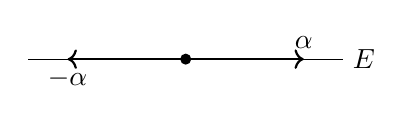
\begin{tikzpicture}
        \draw[-] (-2,0) -- (2,0) node[right] {$E$};
        \draw[->,thick] (0,0) -- (1.5,0) node[above] {$\alpha$};
        \draw[->,thick] (0,0) -- (-1.5,0) node[below] {$-\alpha$};
        \fill (0,0) circle (2pt);
    \end{tikzpicture}
\end{center}
となる.\\
$\ell = 2$~のルート系は以下の$A_1 \times A_1,~A_2,~B_2,~G_2$~の4種類しか存在しないことが知られている.\\
これは,~ルート系の定義(R4)~の整数性が強く制限を与えるためである.\\
階数2のルート系のWely群は,~位数$2n$の二面体群$D_{n}$を考えればよい.~これは,~$\theta$違うルート$\alpha,~\beta$~に対して,~$\sigma_\alpha \sigma_\beta$~という銅鏡が空間を$2\theta$~回転させることから分かる.\\
二面体群の代数的な定義は以下で与えられる.
\begin{equation*}
        D_{n} = \langle r, s \mid r^2 = s^2 = (rs)^n  \rangle
\end{equation*}
$A_1 \times A_1$~のWely群の生成元は互いに直交する銅鏡$\sigma_\alpha,~\sigma_\beta$~であるので,~これは可換となる.~よって,
\begin{equation*}
    \mathcal{W}_{A_1 \times A_1} =\ev{\sigma_\alpha,\sigma_\beta}=  \{1, \sigma_\alpha, \sigma_\beta, \sigma_\alpha \sigma_\beta\} \cong D_2
\end{equation*}
となる.\\\\
$A_2$~のWely群の生成元は互いに60°の角度をなす銅鏡$\sigma_\alpha,~\sigma_\beta$~である.~よって,
\begin{equation*}
    \mathcal{W}_{A_2} \cong D_3 \cong S_3
\end{equation*}
となる.~これは非可換群となり,~対称群$S_3$~と同型であることは正三角形の頂点の回転を考えれば分かる.\\\\
$B_2$~のWely群の生成元は互いに45°の角度をなす銅鏡$\sigma_\alpha,~\sigma_\beta$~である.~よって,
\begin{equation*}
    \mathcal{W}_{B_2} \cong D_4
\end{equation*}
となる.\\\\
$G_2$~のWely群の生成元は互いに30°の角度をなす銅鏡$\sigma_\alpha,~\sigma_\beta$~である.~よって,
\begin{equation*}
    \mathcal{W}_{G_2} \cong D_6
\end{equation*}
となる.
\newpage
\subsubsection{Pairs of roots}
ルート系の定義(R4)~$\ev{\beta,\alpha} \in \mathbb{Z}$~はルート系の構造を強く制限する.\\
$\alpha,~\beta \in \Phi$~のなす角を$\theta$~とすると,~
\begin{equation*}
    \ev{\beta,\alpha} = \frac{2(\beta,\alpha)}{(\alpha,\alpha)} = 2\frac{\|\beta\|}{\|\alpha\|}\cos\theta \in \mathbb{Z}
\end{equation*}
\begin{equation*}
    \ev{\alpha,\beta}\ev{\alpha,\beta} = 4\cos^2 \theta \in \mathbb{Z}
\end{equation*}
が成り立つ必要がある.~$0\leq \cos^2 \theta \leq 1$~であることから,~$\ev{\alpha,\beta}$の取り得る整数値は限られる.~\\
$\alpha \neq \beta,~\|\alpha\| \leq \|\beta\|$~としたとき,~$\ev{\alpha,\beta} \leq \ev{\beta,\alpha}$~となるので,~可能なペアは表1のようになる.\\
\begin{table}[htbp]
  \centering
  \caption{取れるルートのペア}
  \begin{tabular}{ccccc}
    \hline
    $\langle \alpha, \beta \rangle$ & $\langle \beta, \alpha \rangle$ & $\theta$ & $\|\beta\|^2 / \|\alpha\|^2$ & $\ell=2$の場合のルート系の型 \\
    \hline
    $0$ & $0$ & $\pi/2$ & undetermined & $A_1 \times A_1$ \\
    $1$ & $1$ & $\pi/3$ & $1$ & $A_2$ \\
    $-1$ & $-1$ & $2\pi/3$ & $1$ & $A_2$ \\
    $1$ & $2$ & $\pi/4$ & $2$ & $B_2$ \\
    $-1$ & $-2$ & $3\pi/4$ & $2$ & $B_2$ \\
    $1$ & $3$ & $\pi/6$ & $3$ & $G_2$ \\
    $-1$ & $-3$ & $5\pi/6$ & $3$ & $G_2$ \\
    \hline
  \end{tabular}
\end{table}

\textbf{これは$\ell=2$のルート系だけの話ではなく,~一般次元のルート系のルートのペアに対して一般に言えることである.}\\
この表から以下の補題が得られる.
\begin{mylemma}{9.4}
    $\alpha,~\beta$を互いにスカラー倍でないルートとする.~\\
    ・$(\alpha,\beta) > 0 \Rightarrow \alpha - \beta \in \Phi$\\
    ・$(\alpha,\beta) < 0 \Rightarrow \alpha + \beta \in \Phi$\\
    が成り立つ.
\end{mylemma}
\begin{myproof}
    1番目が成立すれば,~$\beta \to -\beta$とすることで2番目も成立する.\\
    $(\alpha,\beta)>0 \Leftrightarrow \ev{\alpha,\beta} >0$~より,~$\|\alpha\| \leq \|\beta\|$~の仮定がない場合にも表1から,~$\ev{\alpha,\beta},~\ev{\beta,\alpha}$~のどちらかは$1$となることが分かる.\\
    $\ev{\alpha,\beta} = 1$~のとき,~$\sigma_\beta(\alpha) = \alpha - \beta \in \Phi$~であるので,~$\alpha - \beta \in \Phi$~が示される.\\
    $\ev{\beta,\alpha} = 1$~のとき,~上より,~$\beta - \alpha \in \Phi$~であり,~$\sigma_{\beta-\alpha}(\beta-\alpha) = -(\beta-\alpha) = \alpha-\beta \in \Phi$~となるので,~示された.
\end{myproof}
この補題の応用として,~比例しないルート$\alpha,~\beta$~を考える.\\
$\alpha$-string though $\beta$という$\Phi$~の部分集合を
\begin{equation*}
    \{\beta + i\alpha \in E \mid i \in \mathbb{Z}\} \cap \Phi
\end{equation*}
で定義する.~$\beta + i \alpha$~がルートとなる最大/最小の整数$i$をそれぞれ$q,-r$~とする.~このとき,~$\alpha$-string through $\beta$~は途切れないことを示せる.\\
もし,~$\alpha$-string through $\beta$~の区間$(-r \leq i \leq q)$に$\beta +i\alpha \notin \Psi$~となる整数$i$が存在するならば,~$p <s$で
\begin{equation*}
    \beta + p\alpha \in \Phi,~\beta + s\alpha \in \Phi,~\beta + (p+1)\alpha \notin \Phi,~\beta + (s-1)\alpha \notin \Phi
\end{equation*}
となる整数$p,~s$を取ることができる.~Lemma~9.4~の対偶を考えると
\begin{equation*}
    (\beta + p\alpha)+\alpha \neq \Phi \Rightarrow (\beta + p\alpha, \alpha) \geq 0
\end{equation*}
\begin{equation*}
    (\beta + s\alpha) - \alpha \neq \Phi \Rightarrow (\beta + s\alpha, \alpha) \leq 0
\end{equation*}
となる.~しかし,~$(\alpha,\alpha) >0$~であることから,~$p<s$~に矛盾する.\\
よって,~$\alpha$-string through $\beta$~は途切れず,~$\beta-r\alpha,~\beta-(r-1)\alpha,~\cdots,~\beta+q\alpha$~がすべてルートであることが示された.\\
次に,~$\alpha$-string through $\beta$~は銅鏡$\sigma_\alpha$~で不変になることが示せる.\\
$-r \leq i \leq q$~を満たす任意の$i$に対して,~(R3)より
\begin{equation*}
    \begin{split}
        \sigma_\alpha (\beta + i\alpha) &= \beta - \ev{\beta,\alpha}\alpha + i(\alpha - \ev{\alpha,\alpha}\alpha)\\
        &= \beta - (-\ev{\beta,\alpha}-i)\alpha \in \Psi
    \end{split}
\end{equation*}
となる.~$-\ev{\beta,\alpha}-i \in \mathbb{Z}$~であることから,~$\sigma_\alpha (\beta + i\alpha)$~も$\alpha$-string through $\beta$~の要素である.\\
よって,~$\alpha$-string through $\beta$~は銅鏡$\sigma_\alpha$~で不変であり,~銅鏡の作用によってstringを反転させることが分かる.\\
特に,~$i =q$~の場合には
\begin{equation*}
    \sigma_\alpha (\beta + q\alpha) = \beta + (-\ev{\beta,\alpha}-q)\alpha = \beta - r\alpha
\end{equation*}
となる.~よって,~$\ev{\beta,\alpha} = r-q$~が示された.\\
表1より,~$\| \ev{\beta,\alpha} \| = \| r-q \| \leq 3 $~であることが分かる.\\
すなわち,~$\alpha$-string through $\beta$~の長さは4以下となる.~まとめると以下の系が得られる.
\begin{mycor}{9.5}
    ルート系に対して\\
    ・$\alpha$-string through $\beta$~は$\beta - r\alpha,~\beta-(r-1)\alpha,~\cdots,~\beta+q\alpha$~の形で途切れずに存在する.\\
    ・$\alpha$-string through $\beta$~は銅鏡$\sigma_\alpha$~で不変であり,~$\sigma_\alpha$~の作用によってstringを反転させる.\\
    ・$\ev{\beta,\alpha} = r-q$~であり,~ $\alpha$-string through $\beta$~の長さは4以下である.
\end{mycor}
\begin{myproof}
    文中で証明済み.
\end{myproof}
\newpage
\subsection{Simple roots and Weyl group}
\subsubsection{Bases and Wely chambers}
\begin{mydef}{10.1.1}
    $Phi$の部分集合$\Delta$~がbaseであるとは,~以下の条件を満たすことをいう.\\
    (B1)~$\Delta$~は$E$の基底.~すなわち,~$\text{span}_\mathbb{R}(\Delta) = E$~であり,~$\Delta$~の要素は線形独立である.\\
    (B2)~$\forall \beta \in \Phi$~に対して,~$\beta$~は整数係数$k_\alpha$~を用いて
    \begin{equation*}
        \beta = \sum_{\alpha \in \Delta} k_\alpha \alpha
    \end{equation*}
    で一意的に表せて,~$k_\alpha$~はすべて非負であるか,~すべて非正である.
\end{mydef}
\begin{mydef}{10.1.2}
    ・$\Delta$~に属するルートを\textbf{単純ルート}(simple root)~という.\\
    ・$\beta = \sum_{\alpha \in \Delta} k_\alpha \alpha \in \Phi$~に対して,~$\Delta$~に関する高さ(height)~を
    \begin{equation*}
        \text{ht}(\beta) = \sum_{\alpha \in \Delta} k_\alpha \in \mathbb{Z}
    \end{equation*}
    と定義する.~これは,~$\Delta$を固定すれば一意に定まる.\\
    ・$\forall \alpha \in \Delta$~に対して,~$k_\alpha \geq 0$,~($k_\alpha \leq 0$)のとき,~$\beta$~をpositive,~(negative) root~という.\\
    positive root~を$\beta \succ 0$~,~negative root~を$\beta \prec 0$~と表す.~positive root~の集合を$\Phi^+$~,~negative root~の集合を$\Phi^-$~と表す.
\end{mydef}
展開の一意性とルート系の性質から,~$\Phi^+ = -\Phi^-$~であることが分かる.\\
$\mu,~\lambda \in E$~に対して,~$\mu \prec \lambda$~を
\begin{equation*}
    \lambda - \mu = \sum_{\alpha \in \Delta} k_\alpha \alpha,~~k_\alpha \in \mathbb{Z}_{\geq 0}
\end{equation*}
で定義すると,~$\prec$~は$E$上に半順序を定めることができる.\\
\begin{myproof}
    $\Delta$~が$E$の基底であることから,~$\forall x \in E$~は
    \begin{equation*}
        x = \sum_{\alpha \in \Delta} x_\alpha \alpha,~~x_\alpha \in \mathbb{R}
    \end{equation*}
    と一意的に表せる.~\\
    \textbf{反射律}\\
    \begin{equation*}
        x - x = \sum_{\alpha \in \Delta} (x_\alpha - x_\alpha) \alpha = 0
    \end{equation*}
    であり,~$\forall \alpha \in \Delta$~に対して,~$x_\alpha - x_\alpha = 0 \in \mathbb{R}_{\geq 0}$~であることから反射律が成り立つ.\\
    \textbf{推移律}\\
    $x \prec y$~と~$y \prec z$~のとき,~
    \begin{equation*}
        y - x = \sum_{\alpha \in \Delta} (y_\alpha - x_\alpha) \alpha,~~y_\alpha - x_\alpha \in \mathbb{Z}_{\geq 0}
    \end{equation*}
    \begin{equation*}
        z - y = \sum_{\alpha \in \Delta} (z_\alpha - y_\alpha) \alpha,~~z_\alpha - y_\alpha \in \mathbb{Z}_{\geq 0}
    \end{equation*}
    が成り立つので,~これらを足し合わせると
    \begin{equation*}
        z - x = (z - y) + (y - x) = \sum_{\alpha \in \Delta} (z_\alpha - x_\alpha) \alpha
    \end{equation*}
    $z_\alpha - x_\alpha = (z_\alpha - y_\alpha) + (y_\alpha - x_\alpha) \in \mathbb{Z}_{\geq 0}$~であることから,~$x \prec z$~が示される.\\
    \textbf{反対称律}\\
    $x \prec y$~と~$y \prec x$~のとき,~
    \begin{equation*}
        y - x = \sum_{\alpha \in \Delta} (y_\alpha - x_\alpha) \alpha,~~y_\alpha - x_\alpha \in \mathbb{Z}_{\geq 0}
    \end{equation*}
    かつ
    \begin{equation*}
        x - y = \sum_{\alpha \in \Delta} (x_\alpha - y_\alpha) \alpha,~~x_\alpha - y_\alpha \in \mathbb{Z}_{\geq 0}
    \end{equation*}
    が成り立つので,~$\forall \alpha \in \Delta$~に対して,~$y_\alpha - x_\alpha = 0$~であることが分かる.~よって,~$x = y$~が示された.\\
    しかし,~これは全順序を定めない.~任意に$x,y \in E$~を取ったとき,~$x_\alpha - y_\alpha$~の符号がすべて同じとは限らないためである.~よって,~$E$上に半順序を定めることが示された.
\end{myproof}
例えば,~$A_1 \times A_1$型のルート系を考える.~$E = \mathbb{R}^2$~,$\Phi = \{\pm e_x, \pm e_y\}$~であるので,~$\Delta = \{e_x, e_y\}$~はbaseである.~このとき,~$x = 2e_x +3 e_y$~,~$y = 3e_x + 2e_y$~とすると,~$x \prec y$~でも~$y \prec x$~でもないことが分かる.~\\
$ x \succ y$が成り立つ領域は$y$を中心として右上に伸びる領域であり,~$y \succ x$~が成り立つ領域は$y$を中心として左下に伸びる領域,~順序が定まらない領域は$y$を中心とする右下と左上の領域であることが分かる.~これを図示すると以下のようになる.
\begin{figure}[htbp]
  \centering
  \begin{tikzpicture}[scale=1.2]
    % 領域の定義と塗りつぶし
    \fill[blue!10] (3,2) rectangle (5.5,4.5);   % \succ y の領域
    \fill[red!10]  (0.5,0.5) rectangle (3,2);   % \prec y の領域
    \fill[gray!15] (0.5,2) rectangle (3,4.5);   % 順序が定まらない領域 (左上)
    \fill[gray!15] (3,0.5) rectangle (5.5,2);   % 順序が定まらない領域 (右下)

    % 境界線 (yを通る平行線)
    \draw[dashed, thin] (0.5,2) -- (5.5,2);
    \draw[dashed, thin] (3,0.5) -- (3,4.5);

    % 基底 (軸) の描画
    \draw[->, >=stealth, thick] (0,0) -- (6,0) node[right] {$e_x$};
    \draw[->, >=stealth, thick] (0,0) -- (0,5) node[above] {$e_y$};

    % グリッド線
    \draw[very thin, lightgray, step=1.0] (0,0) grid (5.5,4.5);

    % 点 y
    \filldraw[black] (3,2) circle (2pt) node[below right] {$y$};

    % 点 x (左上の順序が定まらない領域内)
    \filldraw[black] (2,3) circle (2pt) node[above left] {$x$};

    % 領域ラベル
    \node at (4.25, 3.25) {$x \succ y$};
    \node at (1.75, 1.25) {$x \prec y$};
    \node at (1.25, 3.75) {？};
    \node at (4.25, 1.25) {？};
  \end{tikzpicture}
  \caption{$A_1 \times A_1$ 型ルート系における半順序の領域と点 $x, y$ の関係}
  \label{fig:root_order}
\end{figure}
baseの定義を述べたが,~それはbaseの存在を保証するものではない.\\
9.3 Figer1~の$\alpha,~\beta$~はbaseになる.~ここで,~$\alpha$~と$\beta$の成す角は鈍角,~すなわち,~$(\alpha, \beta) \leq 0$~であることに注意する.
\begin{mylemma}{10.1.3}
    $\Delta$が$\Phi$のbaseであるとき,~任意の相異なる$\alpha,~\beta \in \Delta$~に対して,~$(\alpha, \beta) \leq 0$~が成り立ち,~$\alpha - \beta \notin \Phi$~となる.
\end{mylemma}
\begin{myproof}
    対偶を考える.~$(\alpha, \beta) > 0$~のとき,~Lemma~9.4~より,~$\alpha - \beta \in \Phi$~となる.~しかし,~$\alpha -\beta = 1\cdot \alpha + (-1)\cdot \beta$~であることから,~baseの定義(B2)~を満たさない.~よって,~$\Delta$~はbaseではないので,~示された.\\
\end{myproof}
各$\gamma \in E$~に対して
\begin{equation*}
    \Phi^+(\gamma) = \{\alpha \in \Phi \mid (\alpha, \gamma) > 0\}
\end{equation*}
\begin{equation*}
    \Phi^-(\gamma) = \{\alpha \in \Phi \mid (\alpha, \gamma) < 0\}
\end{equation*}
と定義する.~有限個の超平面 $P_\alpha$ ($\alpha \in \Phi$) の和集合を考えたとき,~$\bigcup_{\alpha \in \Phi} P_\alpha$~は$E$~を埋め尽くさない.
\begin{mydef}{10.1.4}
    ・$\gamma \in E$~がregularであるとは,~$\gamma \in E\setminus \bigcup_{\alpha \in \Phi} P_\alpha$~であることをいう.~\\
    ・$\gamma \in E$~がsignificantであるとは,~$\gamma \in \bigcup_{\alpha \in \Phi} P_\alpha$~であることをいう.
\end{mydef}
$\gamma$~がregularであるとき,~$\forall \alpha \in \Phi$~に対して,~$(\alpha, \gamma) \neq 0$~である.~ルート系の定義(R2)より,
\begin{equation*}
    \Phi = \Phi^+(\gamma) \cup (-\Phi^+(\gamma))
\end{equation*}
が成立する.~
\begin{mydef}{10.1.5}
    $\alpha \in \Phi^+(\gamma)$~に対して\\
    ・$\alpha$~がdecomposableであるとは,~$\alpha = \beta_1 + \beta_2$~となる$\beta_1,~\beta_2 \in \Phi^+(\gamma)$~が存在することをいう.~\\
    ・$\alpha$~がindecomposableであるとは,~$\alpha$~がdecomposableでないことをいう.
\end{mydef}
任意のルート系にはbaseが存在することを具体的な構成によって示す.
\begin{mythm}{10.1.6}
    $\gamma \in E$~をregularとして,~$\Delta(\gamma)$~を$\Phi^+(\gamma)$~のindecomposableな要素全体の集合とする.~\\
    このとき,~$\Delta(\gamma)$~は$\Phi$~のbaseとなり,~任意のbaseは$\Delta(\gamma)$~の形で表せる.
\end{mythm}
\begin{myproof}
    (1)~$\Phi^+(\gamma)$の任意の元は$\Delta(\gamma)$~の$\mathbb{Z}_{\geq 0}$-線形結合で表せることを背理法によって示す.\\
    仮に,~$\alpha \in \Phi^+(\gamma)$~が$\Delta(\gamma)$~の$\mathbb{Z}_{\geq 0}$-線形結合で表せないとする.~そのような$\alpha$~のなかで$(\gamma,\alpha)$~が最小なものを取り,~$\alpha_0$とする.~$\alpha_0 \in \Delta(\gamma)$~であるとすると,~係数が$1$となってしまうので非負整数係数の和で表せてしまう.\\
    よって,~$\alpha_0$~はdecomposableであり,~すなわち,~ある$\beta_1,~\beta_2 \in \Phi^+(\gamma)$~が存在して,~$\alpha_0 = \beta_1 + \beta_2$~となる.~
    このとき,~$(\gamma, \alpha_0) = (\gamma, \beta_1) + (\gamma, \beta_2)$~であることから,~$(\gamma, \beta_i) < (\gamma, \alpha_0)$~が成り立つ.~$\alpha_0$~は$(\gamma,\alpha)$~が最小なものの1つであることから,~$\beta_i$~は$\Delta(\gamma)$~の$\mathbb{Z}_{\geq 0}$-線形結合で表せるはずであるので,~$\alpha_0 = \beta_1 + \beta_2$~も$\Delta(\gamma)$~の$\mathbb{Z}_{\geq 0}$-線形結合で表せることになる.~
    これは,~$\alpha_0$~が$\Delta(\gamma)$~の$\mathbb{Z}_{\geq 0}$-線形結合で表せないとした仮定に矛盾する.~よって,~$\Phi^+(\gamma)$の任意の元は$\Delta(\gamma)$~の$\mathbb{Z}_{\geq 0}$-線形結合で表せることが示された.\\
    (2)~$\alpha \neq \beta$~を満たす任意の$\alpha,~\beta \in \Delta(\gamma)$~に対して,~$(\alpha, \beta) \leq 0$~であることを背理法によって示す.\\
    $(\alpha, \beta) >0$~のとき,~Lemma~9.4から,~$\alpha -\beta,~\beta -\alpha \in \Phi$~なので,~$\alpha -\beta $か$\beta-\alpha$~のどちらかは$\Phi^+(\gamma)$~に属することになる.\\
    $\alpha - \beta \in \Phi^+(\gamma)$~のとき,~$\alpha = (\alpha - \beta) + \beta$~となるので,~$\alpha$~はdecomposableである.~$\beta - \alpha \in \Phi^+(\gamma)$~のときも同様に考えると~$\beta$~はdecomposableとなる.~いずれの場合も,~$\alpha$~か$\beta$~のどちらかがdecomposableとなってしまうので矛盾.~よって示された.\\
    (3)~$\Delta(\gamma)$~の元は互いに線形独立であることを示す.\\
    $\sum_{\alpha \in \Delta(\gamma)} r_\alpha \alpha = 0$~となるような$c_\alpha \in \mathbb{R}$~を取る.~$r_\alpha \geq 0$~となるものを$s_\alpha$,~$r_\alpha < 0$~となるものを$r_\alpha = -t_\alpha$~とする.~このとき,~$\sum_{\alpha \in \Delta(\gamma)} s_\alpha \alpha = \sum_{\alpha \in \Delta(\gamma)} t_\alpha \alpha$~となる.~(2)より
    \begin{equation*}
        \left(\sum_{\alpha \in \Delta(\gamma)} s_\alpha \alpha, \sum_{\beta \in \Delta(\gamma)} s_\beta \beta\right) = \sum_{\alpha,~\beta \in \Delta(\gamma)} s_\alpha t_\beta (\alpha, \beta) \leq 0
    \end{equation*}
    となるが,~内積の正定値性から,~$\sum_{\alpha \in \Delta(\gamma)} s_\alpha \alpha = 0$~が示される.~同様にして,~$\sum_{\alpha \in \Delta(\gamma)} t_\alpha \alpha = 0$~も示される.~よって,
    \begin{equation*}
        0 = \left( \gamma, \sum_{\alpha \in \Delta(\gamma)} s_\alpha \alpha\right) = \sum_{\alpha \in \Delta(\gamma)} s_\alpha (\gamma, \alpha)
    \end{equation*}
    となる.~$\alpha \in \Delta(\gamma)$~は$\Phi^+(\gamma)$~の要素であることから,~$(\gamma, \alpha) > 0$~であることが分かる.~$s_\alpha \geq 0$~であることから,~$\forall \alpha \in \Delta(\gamma)$~に対して$s_\alpha = 0$~が示される.~同様にして,~$t_\alpha = 0$~も示されるので,~$r_\alpha = 0$~が示される.~よって,~$\Delta(\gamma)$~の元は互いに線形独立であることが示された.\\
    (4)~$\Delta(\gamma)$~は$\Phi$~のbaseであることを示す.\\
    $\Phi = \Phi^+(\gamma) \cup (-\Phi^+(\gamma))$~であることから,~(3)より,B2が示せて,~(1)より,B1も示せるので,~$\Delta(\gamma)$~は$\Phi$~のbaseであることが示された.\\
    (5)~任意のbase$\Delta$はある$\gamma \in E : regular$~を用いて$\Delta = \Delta(\gamma)$~の形で表せることを示す.\\
    与えられた$\Delta$~に対して,~$(\gamma, \Delta) > 0$~を満たす$\gamma \in E$~を取ることができる.~(B2)より,~$\gamma$はregularであり,~$\forall \beta = \sum_{\alpha \in \Delta} \beta_\alpha \alpha \in \Phi^+$~に対して,~$(\gamma, \beta) = \sum_{\alpha \in \Delta} k_\alpha (\gamma, \alpha) > 0$~が成立して,~$\beta \in \Phi^+(\gamma)$~となる.~\\
    すなわち,~$\Phi^+ \subset \Phi^+(\gamma)$~である.~同様にして,~$\Phi^- \subset (-\Phi^+(\gamma))$~も示される.~$\Phi = \Phi^+ \cup \Phi^- \subset \Phi^+(\gamma) \cup (-\Phi^+(\gamma))$~であることから,~$\Phi^+ = \Phi^+(\gamma) $~である必要がある.~\\
    仮に,~$\alpha = \beta_1 + \beta_2$~となる$\beta_1,~\beta_2 \in \Phi^+(\gamma)$~で表せたとすると,~$\beta_i = \sum_{\alpha \in \Delta} \beta_{i,\alpha} \alpha$~であることから,~
    \begin{equation*}
        \beta_{1,\alpha} + \beta_{2,\alpha} = 1,~~\beta_{1,\alpha'} + \beta_{2,\alpha'} = 0,~~\forall \alpha' \in \Delta\setminus \{\alpha\}
    \end{equation*}
    となることから,~$(\beta_1, \beta_2) = (0,\alpha) \text{ or } (\alpha,0)$~となる.~いずれの場合も,~$ 0 \notin \Phi^+$~であることから矛盾.~よって,~任意の$\alpha$はindecomposableとなり,~$\Delta \subset \Delta(\gamma)$~であることが示される.~(4)~より,~$\Delta(\gamma)$~は$\Phi$~のbaseであることから,~$\Delta = \Delta(\gamma)$~が示された.\\
\end{myproof}
\newpage
\begin{mydef}{10.1.7}
    ・$E\setminus \bigcup_{\alpha \in \Phi} P_\alpha$~の連結成分の1つのことを\textbf{Weyl chamber}~という.\\
    ・$\gamma \in E$~がregularであるとき,~この$\gamma$~が属するWeyl chamber~を$\mathfrak{C}(\gamma)$と書くことにする.\\
    ・$\Delta = \Delta(\gamma)$~というbaseとregularな$\gamma$の対応が作れることから,~$\mathfrak{C}(\Delta) =\mathfrak{C}(\gamma)$~と書き,~これを$\Delta$に関する基本Weyl chamber~と呼ぶことにする.
\end{mydef}
\textbf{Weyl chamberとbaseについて}\\
$\mathcal{C}(\gamma) = \mathcal{C}(\gamma')$~であるとは,~$\gamma = \gamma'$が任意の$P_\alpha,~\alpha \in \Phi$~の同じ側に属することであり.~$\Phi^+(\gamma) = \Phi^+(\gamma')$~であることと同値である.~$\Delta(\gamma)$~は$\Phi^+(\gamma)$~のindecomposableな要素全体の集合であることから,~$\Delta(\gamma) = \Delta(\gamma')$~であることと同値である.~\\
よって,~Weyl chamber~とbase~の間には1対1対応があることが分かる.~
\begin{equation*}
    \mathcal{C}(\gamma) \leftrightarrow \Delta(\gamma)
    \leftrightarrow \Delta
\end{equation*}
$\mathfrak{C}(\Delta)$~とは,~任意の$\alpha \in \Delta$~に対して$(\gamma,\alpha)>0$~であるような$\gamma \in E$~が属する集合である.\\
$A_2$型のルート系を考えると,~以下のような領域になる.
\begin{center}
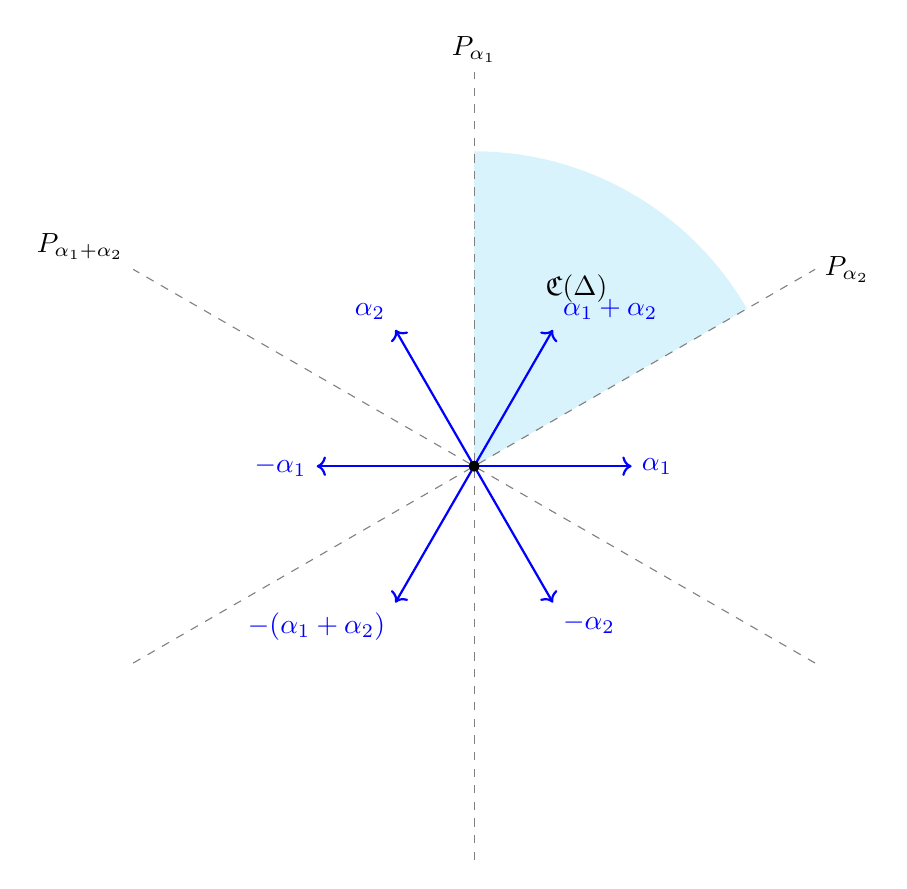
\begin{tikzpicture}[scale=2]
    % 基本ウェイル領域 C(\Delta) の塗りつぶし
    \fill[cyan!15] (0,0) -- (30:2) arc (30:90:2) -- cycle;

    % 各ルートに直交する超平面（境界線）
    \draw[dashed, gray] (-150:2.5) -- (30:2.5) node[right, text=black] {$P_{\alpha_2}$};
    \draw[dashed, gray] (-90:2.5) -- (90:2.5) node[above, text=black] {$P_{\alpha_1}$};
    \draw[dashed, gray] (-30:2.5) -- (150:2.5) node[above left, text=black] {$P_{\alpha_1+\alpha_2}$};

    % A2型のルート
    \draw[->, thick, blue] (0,0) -- (0:1) node[right] {$\alpha_1$};
    \draw[->, thick, blue] (0,0) -- (120:1) node[above left] {$\alpha_2$};
    \draw[->, thick, blue] (0,0) -- (60:1) node[above right] {$\alpha_1+\alpha_2$};
    \draw[->, thick, blue] (0,0) -- (180:1) node[left] {$-\alpha_1$};
    \draw[->, thick, blue] (0,0) -- (300:1) node[below right] {$-\alpha_2$};
    \draw[->, thick, blue] (0,0) -- (240:1) node[below left] {$-(\alpha_1+\alpha_2)$};

    % 領域のラベル
    \node at (60:1.3) {$\mathfrak{C}(\Delta)$};
    
    % 原点
    \fill (0,0) circle (1pt);
\end{tikzpicture}
\end{center}
Weyl群は,~$\Phi$~のルートに対する銅鏡によって生成される群である.~このとき,~Weyl群はWely chamberを別のWeyl chamberに移す.~\\
このことから,~特に以下の2つが得られる.\\
\begin{mylemma}{10.1.8}
    $\forall \sigma \in \mathcal{W},~\forall \gamma \in E$~:~regular~に対して,~\\
    (1)~$\sigma(\Delta(\gamma)) = \Delta(\sigma(\gamma))$\\
    (2)~$\sigma(\Delta)$~は$\Phi$~のbase.
\end{mylemma}
\begin{myproof}
    (1)~$\sigma$~は直交変換であることから,~
    \begin{equation*}
        \begin{split}
            \sigma(\Phi^+(\gamma)) &= \{ \sigma(\alpha) \in \Phi \mid (\gamma,\alpha) = (\sigma(\gamma), \sigma(\alpha)) > 0 \} \\
            &= \{ \alpha' \in \Phi \mid (\sigma(\gamma), \alpha') > 0 \} = \Phi^+(\sigma(\gamma))
        \end{split}
    \end{equation*}
    となるので,~成立する.\\
    (2)~$\Delta = \Delta(\gamma)$~という$\gamma \in E$~:~regular~が存在して,~$\sigma(\Delta) = \sigma(\Delta(\gamma)) = \Delta(\sigma(\gamma))$~であることから,~Theorem 10.1.6より,~$\sigma(\Delta)$~は$\Phi$~のbaseであることが示された.
\end{myproof}
\newpage
\subsubsection{Lemmas on simple roots}
$\Phi$のbaseを任意に1つ固定して,~$\Delta$~とする.\\
\begin{mylemma}{10.2.1 A}
    $\alpha$がpositive root かつ non simple root $(\alpha \in \Phi^+ \setminus \Delta)$~であるとき,~ある$\beta \in \Delta$~が存在して,~$\alpha - \beta \in \Phi$~となる.\\
    また,~このとき,~$\alpha - \beta$~はpositive rootである.
\end{mylemma}
\begin{myproof}
    $\forall \beta \in \Delta$~に対して,~$(\alpha,\beta)\leq 0$を仮定する.\\
    Theorem~10.2~Step3~と同様の議論をすると,~$\Delta \cup \{\alpha\}$~が線形独立となるが,~これは $\Delta$ が $E$ の基底であることに矛盾する.~よって,~$(\alpha, \beta) > 0$ となる $\beta \in \Delta$ が存在する.\\
    $\alpha \notin \Delta$ より $\alpha \neq \pm \beta$ なので,~Lemma 9.4 から $\alpha - \beta \in \Phi$ となる.
    またこのとき、$\alpha$ を base で展開すると $\alpha = \sum_{\gamma \in \Delta} k_\gamma \gamma \quad (k_\gamma \in \mathbb{Z}_{\ge 0})$ と書ける.
    $\alpha \neq \beta$ であるため、$\alpha$ には $\beta$ 以外の成分も存在する~(すなわち $\gamma \neq \beta$ となる $\gamma$ について $k_\gamma > 0$ となるものが存在する)~.
    $\alpha - \beta$ の展開における $\gamma$ ($\gamma \neq \beta$) の係数は正のまま残るため、ルートの性質からすべての係数は同符号となり,~$\alpha - \beta \succ 0$~(positive)~となる.
\end{myproof}
\begin{mycor}{10.2.2}
    任意の $\beta \in \Phi^+$ は $\alpha_1 + \dots + \alpha_k \quad (\alpha_i \in \Delta)$ (重複を許す)~の形に書ける.\\
    このとき,~各部分和 $\alpha_1 + \dots + \alpha_l \quad (1 \le l \le k)$ は常にrootとなる.
\end{mycor}
\begin{myproof}
    $\text{ht}(\beta) = 1$ のとき.~$\beta = \alpha_1 \in \Delta \subset \Phi$ より明らか.\\
    $\text{ht}(\beta) > 1$ のとき,~$\beta \in \Phi^+ \setminus \Delta$ であるので,~Lemma A を用いて $\beta - \alpha_k \in \Phi^+$ となる $\alpha_k \in \Delta$ を取り出す操作を繰り返すことで帰納的に示せる.
\end{myproof}
\begin{mylemma}{10.2.3 B}
    $\alpha$ が simple root ならば,~$\sigma_\alpha$ は $\alpha$ 以外の $\Phi^+$ 上で置換となる.\\
    すなわち,~$\forall \alpha \in \Delta \cap \Phi$ に対して,~$\sigma_\alpha \in GL(E)$ は
    \begin{equation*}
        \sigma_\alpha(\Phi^+ \setminus \{\alpha\}) = \Phi^+ \setminus \{\alpha\}
    \end{equation*}
    を満たす。
\end{mylemma}
\begin{myproof}
    $\beta \in \Phi^+ \setminus \{\alpha\}$ とし,~$\beta = \sum_{\gamma \in \Delta} k_\gamma \gamma \quad (k_\gamma \in \mathbb{Z}_{\ge 0})$ とおく.
    鏡映の定義より $\sigma_\alpha(\beta) = \beta - \langle \beta, \alpha \rangle \alpha$ となる.
    一般に $\sigma_\alpha(\beta) \in \Phi$ であり、$\beta$ において $\gamma \neq \alpha$ となる $\gamma$ の係数 $k_\gamma$ は正である.
    $\sigma_\alpha(\beta)$ を展開しても、$\alpha$ 以外の成分の係数 $k_\gamma$ は変化しないため正のままである.~ルートの性質からすべての係数は同符号となるため,~$\sigma_\alpha(\beta) \in \Phi^+$ である.
    また、$\sigma_\alpha(-\alpha) = \alpha \neq \sigma_\alpha(\beta)$ より、$\sigma_\alpha(\beta) \neq \alpha$.
    以上より、$\sigma_\alpha(\beta) \in \Phi^+ \setminus \{\alpha\}$ が示された.
\end{myproof}
\begin{mycor}{10.2.4}
    $\delta = \frac{1}{2} \sum_{\beta \in \Phi^+} \beta$ とすると,~任意の $\alpha \in \Delta$ に対して $\sigma_\alpha(\delta) = \delta - \alpha$ が成り立つ.
\end{mycor}
\begin{myproof}
    Lemma B より,~$\sigma_\alpha(\Phi^+ \setminus \{\alpha\}) = \Phi^+ \setminus \{\alpha\}$ であるから,~この集合上の和は $\sigma_\alpha$ によって不変である.~よって,
    \begin{equation*}
        \sigma_\alpha(\delta) = \sigma_\alpha\left( \frac{1}{2} \sum_{\beta \in \Phi^+ \setminus \{\alpha\}} \beta + \frac{1}{2} \alpha \right) = \left( \delta - \frac{1}{2}\alpha \right) - \frac{1}{2}\alpha = \delta - \alpha
    \end{equation*}
\end{myproof}
\begin{mylemma}{10.2.5 C}
    $\alpha_1, \dots, \alpha_t \in \Delta$ について,~$\sigma_i = \sigma_{\alpha_i}$ とする.\\
    $\sigma_1 \dots \sigma_{t-1}(\alpha_t) \prec 0$ ならば,~ある $1 \le s < t$ が存在して,~
    \begin{equation*}
        \sigma_1 \dots \sigma_t = \sigma_1 \dots \sigma_{s-1} \sigma_{s+1} \dots \sigma_{t-1}
    \end{equation*}
    が成り立つ.
\end{mylemma}
\begin{myproof}
    $0 \le i \le t-2$ について,~$\beta_i = \sigma_{i+1} \dots \sigma_{t-1}(\alpha_t)$ とし,~$\beta_{t-1} = \alpha_t$ とおく.\\
    仮定より $\beta_0 \prec 0$ かつ $\beta_{t-1} \succ 0$ であるので,~数列を辿る途中で符号が変わる.~よって $\beta_s \succ 0$ となる最小の $s$ を取れる.~(このとき $\beta_{s-1} \prec 0$ となる).\\
    $\beta_s \in \Phi^+$ かつ $\beta_{s-1} = \sigma_s(\beta_s) \prec 0$ となるが,~正ルートを負ルートに移す鏡映 $\sigma_s$ の性質~(Lemma B)により,~$\beta_s = \alpha_s$ でなくてはならない.~($\alpha_s$ 以外であれば正ルートのままとなるため).\\
    よって,~$\beta_s = \sigma_{s+1} \dots \sigma_{t-1}(\alpha_t) = \alpha_s$ である.
    Weyl群の元による鏡映の共役関係~($w \sigma_\alpha w^{-1} = \sigma_{w(\alpha)}$)~から,~$w = \sigma_{s+1} \dots \sigma_{t-1}$ とみなすことで
    \begin{equation*}
        \sigma_s = \sigma_{\alpha_s} = (\sigma_{s+1} \dots \sigma_{t-1}) \sigma_t (\sigma_{s+1} \dots \sigma_{t-1})^{-1}
    \end{equation*}
    $\sigma_i^{-1} = \sigma_i$ であるから,~
    \begin{equation*}
        \sigma_s = (\sigma_{s+1} \dots \sigma_{t-1}) \sigma_t (\sigma_{t-1} \dots \sigma_{s+1})
    \end{equation*}
    となる.~この式の両辺の左から $\sigma_1 \dots \sigma_{s-1}$、右から $\sigma_{s+1} \dots \sigma_t$ を掛けて整理すると,
    \begin{equation*}
        \begin{split}
            \sigma_1 \dots \sigma_t &= \sigma_1 \dots \sigma_{s-1} (\sigma_{s+1} \dots \sigma_{t-1}) \sigma_t (\sigma_{t-1} \dots \sigma_{s+1}) \sigma_{s+1} \dots \sigma_t \\
                &= \sigma_1 \dots \sigma_{s-1} \sigma_{s+1} \dots \sigma_{t-1}
        \end{split}
    \end{equation*}
    が導かれる.~よって示された.
\end{myproof}
\begin{mycor}{10.2.6}
    $\sigma \in \mathcal{W}$~が$\alpha_1, \dots, \alpha_t \in \Delta$~を用いて$\sigma = \sigma_{\alpha_1} \dots \sigma_{\alpha_t}$~と書けるとき,~このような表示のうち$t$~が最小のものに対しては,~$\sigma(\alpha_t) \prec 0$~が成り立つ.
\end{mycor}
\begin{myproof}
    \begin{equation*}
        \sigma(\alpha_t) = \sigma_{\alpha_1} \dots \sigma_{\alpha_{t-1}}\sigma_{\alpha_t}(\alpha_t) = -\sigma_{\alpha_1} \dots \sigma_{\alpha_{t-1}}(\alpha_t) 
    \end{equation*}
    より,~もし$\sigma(\alpha_t) \succ 0$~であれば,~$\sigma_{\alpha_1} \dots \sigma_{\alpha_{t-1}}(\alpha_t) \prec 0$~となる.~このとき,~Lemma C より,~ある $1 \le s < \text{len}(\sigma)$ が存在して,~
    \begin{equation*}
        \sigma_1 \dots \sigma_{\alpha_t} = \sigma_1 \dots \sigma_{s-1} \sigma_{s+1} \dots \sigma_{t-1}
    \end{equation*}
    となり,~より小さい列$\alpha_1, \dots, \alpha_{s-1}, \alpha_{s+1}, \dots, \alpha_{t-1}$~を用いて$\sigma$~を表すことができる.~これは,~$\sigma$~の表現の長さが最小であるという仮定に矛盾する.~よって,~$\sigma(\alpha_t) \prec 0$~が示された.
\end{myproof}
\newpage
\subsubsection{The Weyl group}
\begin{mythm}{10.3.1}
    (a) $\gamma \in E$ を正則 (regular) な元とすると,~ある $\sigma \in \mathcal{W}$ が存在して,~すべての $\alpha \in \Delta$ について $(\sigma(\gamma), \alpha) > 0$ となる.~\\
    (b) $\Delta'$ を $\Phi$ の任意の base とすると,~ある $\sigma \in \mathcal{W}$ が存在して $\sigma(\Delta') = \Delta$ となる.~\\
    (c) 任意の $\alpha \in \Phi$ に対して,~ある $\sigma \in \mathcal{W}$ が存在して $\sigma(\alpha) \in \Delta$ となる.~\\
    (d) Weyl 群 $\mathcal{W}$ は $\sigma_\alpha \ (\alpha \in \Delta)$ により生成される.~\\
    (e) $\sigma(\Delta) = \Delta$ を満たす $\sigma \in \mathcal{W}$ は $\sigma = 1$ のみである.~(すなわち,~Weyl群の作用は自由である.)
\end{mythm}
$\mathcal{W}' \subset \mathcal{W}$ を,~$\Delta$ の元による鏡映 $\sigma_\alpha \ (\alpha \in \Delta)$ により生成される部分群とする.~\\
まず $\mathcal{W}'$ について (a) 〜 (c) が成り立つことを示し,~これを用いて (d) （すなわち $\mathcal{W}' = \mathcal{W}$）を示し,~最後に (e) を証明する.~
\begin{myproof}
    (a)~$\delta = \frac{1}{2} \sum_{\alpha \in \Phi^+} \alpha$ とおき,~$\mathcal{W}'$ は有限群であるから,~$(\sigma(\gamma), \delta)$ が最大になるような $\sigma \in \mathcal{W}'$ をとる.\\
    任意の $\alpha \in \Delta$ について,~群の定義より $\sigma_\alpha \sigma \in \mathcal{W}'$ であるから,~$\sigma$ の最大性により次が成り立つ.~
    \begin{equation*}
        \begin{split}
            (\sigma(\gamma), \delta) &\ge (\sigma_\alpha \sigma(\gamma), \delta) \\
                &= (\sigma(\gamma), \sigma_\alpha(\delta)) \quad (\text{内積の不変性より}) \\
                &= (\sigma(\gamma), \delta - \alpha) \quad (\text{Lemma B の系より}) \\
                &= (\sigma(\gamma), \delta) - (\sigma(\gamma), \alpha)
        \end{split}
    \end{equation*}
    これより,~$(\sigma(\gamma), \alpha) \ge 0$ が得られる.~さらに,~$(\sigma(\gamma), \alpha) = (\gamma, \sigma^{-1}(\alpha))$ であり,~$\gamma$ は正則かつ $\sigma^{-1}(\alpha) \in \Phi$ であるため,~$(\gamma, \sigma^{-1}(\alpha)) \neq 0$ となる.~
    よって,~$(\sigma(\gamma), \alpha) > 0$ が示された.~\\\\
    (b)~$\Delta'$ は base であるから,~ある正則な元 $\gamma' \in E$ を用いて $\Delta' = \Delta(\gamma')$ と表せる.~また,~固定された base $\Delta$ もある正則な元 $\gamma$ を用いて $\Delta = \Delta(\gamma)$ と表される.~\\
    (a) の結果を $\gamma'$ に対して適用すると,~すべての $\alpha \in \Delta$ に対して $(\sigma(\gamma'), \alpha) > 0$ となるような $\sigma \in \mathcal{W}'$ を選ぶことができる.~これは $\sigma(\gamma')$ が $\Delta$ を定義する基本領域に属すること,~すなわち $\Delta(\sigma(\gamma')) = \Delta$ であることを意味する.~
    一方で,~基本性質 $\Delta(\sigma(\gamma')) = \sigma(\Delta(\gamma'))$ より,~$\sigma(\Delta(\gamma')) = \sigma(\Delta')$ となる.~\\
    したがって,~$\sigma(\Delta') = \Delta$ が成り立つ.~\\\\
    (c)~任意の $\alpha \in \Phi$ に対し,~$\alpha$ を含むような base $\Delta'$ が存在することを示せばよい.~それが示されれば,~(b) より $\sigma(\Delta') = \Delta$ となる $\sigma \in \mathcal{W}'$ が存在し,~$\sigma(\alpha) \in \Delta$ が導かれるためである.~
    $k\alpha \in \Phi$ となるのは $k = \pm 1$ のみであるから,~超平面 $P_\alpha = \{ x \in E \mid (x, \alpha) = 0 \}$ は,~他のルート $\beta \neq \pm \alpha$ に直交する超平面 $P_\beta$ の有限和集合には包まれない.~
    よって,~$\gamma \in P_\alpha$ でありながら,~任意の $\beta \neq \pm \alpha$ に対して $\gamma \notin P_\beta$ となるような $\gamma$ をとることができる.~
    この $\gamma$ を $P_\alpha$ に直交する方向へわずかに摂動させた $\gamma' \in E$ を考える.~
    すなわち,~$(\gamma', \alpha) = \varepsilon > 0$ は非常に小さく,~$\beta \neq \pm \alpha$ に対しては $|(\gamma', \beta)| \gg \varepsilon$ となるように $\gamma'$ をとる.~
    このとき $\gamma'$ はどの超平面にも属さないため正則 (regular) であり,~正ルートの集合 $\Phi^+(\gamma')$ と base $\Delta(\gamma')$ を定める.~
    $\alpha \in \Phi^+(\gamma')$ であるが,~内積 $(\gamma', \alpha)$ が他のどの正ルートとの内積よりも小さいため,~$\alpha$ を他の正ルートの和として表すことは不可能である.~
    したがって,~$\alpha$ は indecomposable (分解不可能) なルートであり,~$\alpha \in \Delta(\gamma')$ となる.~
    これにより題意は示された.~\\\\
    (d)~任意の $\alpha \in \Phi$ に対して,~$\sigma_\alpha \in \mathcal{W}'$ を示せば十分である.~\\
    (c) より,~$\beta = \sigma(\alpha) \in \Delta$ となる $\sigma \in \mathcal{W}'$ が存在する.~鏡映の共役の性質 $\sigma_\beta = \sigma \sigma_\alpha \sigma^{-1}$ より,~$\sigma_\alpha = \sigma^{-1} \sigma_\beta \sigma$ と変形できる.~\\
    $\beta \in \Delta$ であるから定義より $\sigma_\beta \in \mathcal{W}'$ であり,~$\sigma \in \mathcal{W}'$ でもあるため,~閉性から $\sigma_\alpha \in \mathcal{W}'$ が従う.~\\\\
    (e)~$\sigma \neq 1$ と仮定する.~(d) より $W$ は simple root の鏡映で生成されるため,~$\sigma = \sigma_{\alpha_1} \dots \sigma_{\alpha_k} \ (\alpha_i \in \Delta)$ と表すことができる.~($k$ が最小になるように表示をとる.~)
    このとき,~Lemma 10.2 C より $\sigma(\alpha_k) = \sigma_1 \dots \sigma_k(\alpha_k) \prec 0$ となる.~しかし,~$\alpha_k \in \Delta \subset \Phi^+$ であり,~$\sigma(\Delta) = \Delta$ は正ルートを正ルートに写すことを意味するため,~矛盾が生じる.~\\
    したがって,~$\sigma = 1$ でなければならない.~
\end{myproof}
\begin{mydef}{10.3.2}
    任意の $\sigma \in \mathcal{W}$ について,~$\sigma = \sigma_{\alpha_1} \dots \sigma_{\alpha_k} \ (\alpha_i \in \Delta)$ と simple root の鏡映の積で表すことができる.~\\
    積の個数 $k$ が最小になるとき,~$k$ を $\sigma$ の長さ (length) と呼び,~$\ell(\sigma) := k$ と定義する.~\\
    この最小個数による表し方を reduced form (既約表示) という.~($\ell(\sigma) = 0 \implies \sigma = 1$ である.~)\\
    また,~$\sigma \in \mathcal{W}$ について,~$\alpha \in \Phi^+$ かつ $\sigma(\alpha) \prec 0$ を満たす正ルート $\alpha$ の個数を $n(\sigma)$ と表す.~
\end{mydef}
\begin{mylemma}{10.3.3 A}
    任意の $\sigma \in \mathcal{W}$ に対して,~$\ell(\sigma) = n(\sigma)$ が成り立つ.~
\end{mylemma}
\begin{myproof}
    (i) $\ell(\sigma) = 0$ のとき:\\
    $\sigma = 1$ であるから,~正ルートを負ルートに写すことはなく $n(\sigma) = 0$ となり,~成立する.\\
    (ii) $\ell(\sigma) > 0$ のとき:\\
    任意の $\tau \in \mathcal{W}$ について,~$\ell(\tau) < \ell(\sigma)$ ならば命題が成立すると仮定する.~\\
    $\sigma$ の reduced form を $\sigma = \sigma_{\alpha_1} \dots \sigma_{\alpha_k} \ (\alpha_i \in \Delta)$ とし,~$\alpha_k = \alpha$ とおく.~\\   
    Lemma 10.2 C より,~$\sigma(\alpha) \prec 0$ である.~また,~Lemma 10.2 B より $\sigma_\alpha$ は $\alpha$ 以外の正ルートを正ルートのまま置換する.~\\
    よって,~$\sigma \sigma_\alpha(\alpha) = \sigma(-\alpha) = -\sigma(\alpha) \succ 0$ となる.~\\
    $\alpha$ 以外の正ルート $\beta \in \Phi^+ \setminus \{\alpha\}$ については,~$\sigma_\alpha(\beta)$ も正ルートであるから,~$\sigma(\beta) \prec 0$ となる元の個数は,~$\sigma \sigma_\alpha$ によって負に写される元の個数よりもちょうど $\alpha$ の分だけ $1$ つ多い.~したがって,~$n(\sigma \sigma_\alpha) = n(\sigma) - 1$ となる.~\\
    一方,~$\sigma \sigma_\alpha = \sigma_{\alpha_1} \dots \sigma_{\alpha_{k-1}}$ であり,~$k$ の最小性から $\ell(\sigma \sigma_\alpha) = \ell(\sigma) - 1$ である.~
    よって $\ell(\sigma \sigma_\alpha) < \ell(\sigma)$ となり帰納法の仮定が適用できるので,~$n(\sigma \sigma_\alpha) = \ell(\sigma \sigma_\alpha)$ が成り立つ.~
    代入して $n(\sigma) - 1 = \ell(\sigma) - 1$ となり,~$n(\sigma) = \ell(\sigma)$ が示された.~
\end{myproof}
\begin{mylemma}{10.3.4 B}
    $\lambda, \mu \in \overline{\mathfrak{C}(\Delta)}$（Weyl chamber の閉包）とする.~ある $\sigma \in W$ について $\sigma \lambda = \mu$ であるならば,~$\sigma$ は $\lambda$ を固定する simple root の鏡映の積として表される.~(特に,~$\mu = \lambda$ となる.~)
\end{mylemma}

\begin{myproof}
    $\ell(\sigma)$ についての帰納法により示す.~\\
    (i) $\ell(\sigma) = 0$ のとき:\\
    $\sigma = 1$ より $\mu = 1 \lambda = \lambda$ となり,~$\sigma$ は自明な積（空な積）として $\lambda$ を固定する.~よって自明に成立する.~\\
    (ii) $\ell(\sigma) > 0$ のとき:\\
    $\ell(\sigma)$ 未満の長さを持つ元について命題の成立を仮定する.~
    Lemma A より $\ell(\sigma) = n(\sigma) > 0$ であるから,~$\sigma(\alpha) \prec 0$ を満たす simple root $\alpha \in \Delta$ が存在する.~\\
    $\mu \in \overline{\mathfrak{C}(\Delta)}$ より,~$\mu$ と任意の正ルートとの内積は非負である.~$-\sigma(\alpha) \succ 0$（正ルート）であるから,~$(\mu, -\sigma(\alpha)) \ge 0$,~すなわち $(\mu, \sigma(\alpha)) \le 0$ となる.~\\
    一方,~Weyl 群の作用に対する内積の不変性を用いると\\
    \begin{equation*}
        (\mu, \sigma(\alpha)) = (\sigma^{-1}\mu, \alpha) = (\lambda, \alpha)
    \end{equation*}
    である.~$\lambda \in \overline{\mathfrak{C}(\Delta)}$ かつ $\alpha \in \Delta$ であるから,~定義より $(\lambda, \alpha) \ge 0$ である.~\\
    これらを合わせると,\\
    \begin{equation*}
        0 \ge (\mu, \sigma(\alpha)) = (\lambda, \alpha) \ge 0
    \end{equation*}
    となり,~$(\lambda, \alpha) = 0$ かつ $(\mu, \sigma(\alpha)) = 0$ が結論づけられる.~\\
    $(\lambda, \alpha) = 0$ より $\lambda$ は超平面 $P_\alpha$ 上の元であるため,~$\sigma_\alpha \lambda = \lambda$ となる.~\\
    これを $\sigma \lambda = \mu$ に代入すると,~$(\sigma \sigma_\alpha) \lambda = \sigma \lambda = \mu$ となる.~\\
    一方で,~$\sigma(\alpha) \prec 0$ であったが,~$\sigma \sigma_\alpha(\alpha) = \sigma(-\alpha) = -\sigma(\alpha) \succ 0$ となる.~$\sigma_\alpha$ は $\alpha$ 以外の正ルートを正ルートに置換するため,~Lemma A の証明と同様の議論から $n(\sigma \sigma_\alpha) = n(\sigma) - 1$ となる.~\\
    したがって,~$\ell(\sigma \sigma_\alpha) = \ell(\sigma) - 1$ である.~\\
    ここで $\tau = \sigma \sigma_\alpha$ とおくと,~$\ell(\tau) < \ell(\sigma)$ かつ $\tau \lambda = \mu$ を満たす.~$\lambda, \mu \in \overline{\mathfrak{C}(\Delta)}$ であるから帰納法の仮定が適用でき,~$\tau$ は $\lambda$ を固定する simple root の鏡映の積として表され,~$\mu = \lambda$ が成り立つ.~\\
    最後に,~$\sigma = \tau \sigma_\alpha$ と表すことができ,~$\tau$ も $\sigma_\alpha$ も $\lambda$ を固定するため,~$\sigma$ 自身も $\lambda$ を固定する simple root の鏡映の積として表されることが示された.~\\
\end{myproof}
\newpage
\subsubsection{Irreducible root systems}
\begin{mydef}{10.4.1}
    ルート系 $\Phi$ が既約 (irreducible) であるとは,~$\Phi = \Phi_1 \sqcup \Phi_2$ かつ $(\Phi_1, \Phi_2) = 0$ を満たすような空でない部分集合 $\Phi_1, \Phi_2$ が存在しないことである.~
\end{mydef}
\begin{mythm}{10.4.2}
    既約なルート系 $\Phi$ の base を $\Delta$ とする.~\\
    $\Phi$ が既約であることと,~$\Delta = \Delta_1 \sqcup \Delta_2$ かつ $(\Delta_1, \Delta_2) = 0$ を満たすような空でない部分集合 $\Delta_1, \Delta_2 \subset \Delta$ が存在しないことは同値である.~
\end{mythm}
\begin{myproof}
    後で書きます...
\end{myproof}
\begin{mylemma}{10.4.3 A}
    $\Phi$ が既約であるならば,~半順序 $\prec$ について $\Phi$ には唯一の極大元$\beta$が存在する.~\\
    さらに,~その極大元を $\beta = \sum_{\alpha \in \Delta} k_\alpha \alpha$ と表したとき,~すべての $\alpha \in \Delta$ に対して $k_\alpha > 0$ が成り立つ.~
\end{mylemma}
\begin{myproof}
    後で書きます...
\end{myproof}
\begin{mylemma}{10.4.4 B}
    $\Phi$ が既約であるならば,~Weyl 群 $\mathcal{W}$ の表現は既約である.\\
    特に,~任意の $\alpha \in \Phi$ の $\mathcal{W}$ による群軌道は $E$ 全体を張る.~
\end{mylemma}
\begin{myproof}
    後で書きます...
\end{myproof}
\begin{mylemma}{10.4.5 C}
    $\Phi$ が既約であるとする.~このとき,~$\Phi$ 内の同じ長さを持つ任意のルートは,~Weyl群 $\mathcal{W}$ の作用によって互いに移り合う.~\\
    また,~$\Phi$ に異なる長さのルートが存在する場合,~その長さは高々2種類に限られる.
\end{mylemma}
\begin{myproof}
    後で書きます...
\end{myproof}
\begin{mylemma}{10.4.6 D}
    $\Phi$ が既約であるとする.~このとき,~Lemma A で与えられた極大元 (maximal root) $\beta_0$ は,~$\Phi$ 内の他のどのルートよりも長い.~(すなわち,~任意の $\alpha \in \Phi$ について $||\beta_0|| \ge ||\alpha||$ が成り立つ.~)
\end{mylemma}
\begin{myproof}
    任意の $\alpha \in \Phi$ に対し,~$(\beta_0, \beta_0) \ge (\alpha, \alpha)$ を示す.~\\
    Weyl 群 $\mathcal{W}$ の作用に対してルートの長さ (内積) は不変であるため,~$\alpha$ を $\mathcal{W} $ の元で移した先の元を改めて $\alpha$ と置くことで,~$\alpha \in \overline{\mathfrak{C}(\Delta)}$ (Weyl chamber の閉包) に属するとしてよい.~\\
    $\beta_0$ は極大元であるから,~$\beta_0 - \alpha \succeq 0$である.~
    基本領域の性質から,~任意の $\gamma \in \overline{\mathfrak{C}(\Delta)}$ はすべての正ルートとの内積が非負であるため,~$(\gamma, \beta_0 - \alpha) \ge 0$ が成り立つ.~\\
    ここで,~極大元 $\beta_0$ 自身も $\overline{\mathfrak{C}(\Delta)}$ に属することに注意する.~(なぜなら,~もしある simple root $\alpha_i$ について $(\beta_0, \alpha_i) < 0$ ならば Lemma 9.4 より $\beta_0 + \alpha_i \in \Phi$ となるが,~これは $\beta_0$ の極大性に矛盾するためである.~)
    また,~仮定より $\alpha \in \overline{\mathfrak{C}(\Delta)}$ である.~上の不等式に $\gamma = \beta_0$ を代入すると,
    \begin{equation*}
        (\beta_0, \beta_0 - \alpha) \ge 0 \implies (\beta_0, \beta_0) - (\beta_0, \alpha) \ge 0 \implies (\beta_0, \beta_0) \ge (\beta_0, \alpha)
    \end{equation*}
    となる.~次に $\gamma = \alpha$ を代入すると,
    \begin{equation*}
        (\alpha, \beta_0 - \alpha) \ge 0 \implies (\alpha, \beta_0) - (\alpha, \alpha) \ge 0 \implies (\beta_0, \alpha) \ge (\alpha, \alpha)
    \end{equation*}
    となる.~これらを合わせると,
    \begin{equation*}
        (\beta_0, \beta_0) \ge (\beta_0, \alpha) \ge (\alpha, \alpha)
    \end{equation*}
    となり,~極大元 $\beta_0$ の長さが任意のルート $\alpha$ の長さ以上であることが示された.
\end{myproof}
\newpage

\subsection{Classification}
この章では,~$(E,\Phi)$を$\text{rank}~\ell$~のルート系,~$\mathcal{W}$をWeyl群,~$\Delta$を$\Phi$のbaseと表記する.
\subsubsection{Cartan matrix of \texorpdfstring{$\Phi$}{Phi}}
単純ルート (simple root) の順序 $(\alpha_1, \dots, \alpha_l)$ を固定する~(ここで $\alpha_i \in \Delta$).
\begin{mydef}{11.1.1}
    行列 $\{(\langle \alpha_i, \alpha_j \rangle\}_{ij} \in M(l, \mathbb{Z})$ を $\Phi$ の \textbf{Cartan 行列} (Cartan matrix) という.\\
    この行列の成分$(\langle \alpha_i, \alpha_j \rangle)$を \textbf{Cartan 整数} という.
\end{mydef}
\vspace{0.5em}
\noindent\textbf{Example: rank 2 のルート系の Cartan 行列}
\begin{itemize}
    \item $A_1 \times A_1$: $\begin{pmatrix} 2 & 0 \\ 0 & 2 \end{pmatrix}$
    \item $A_2$: $\begin{pmatrix} 2 & -1 \\ -1 & 2 \end{pmatrix}$
    \item $B_2$: $\begin{pmatrix} 2 & -2 \\ -1 & 2 \end{pmatrix}$
    \item $G_2$: $\begin{pmatrix} 2 & -1 \\ -3 & 2 \end{pmatrix}$
\end{itemize}
$\langle \alpha_i, \alpha_j \rangle = 2 \frac{(\alpha_i, \alpha_j)}{(\alpha_j, \alpha_j)}$ より, 対角成分 ($i=j$) は $2$ である. 非対角成分はLemma~10.1.3 から非正となる.\\\\
\noindent\textbf{ Cartan 行列は基底 (base) $\Delta$ の選び方によらない.}\\
Weyl 群は基底の集合に推移的に作用する. すなわち, 任意の $\Delta, \Delta'$ に対して, ある $w \in \mathcal{W}$ が存在して $w(\Delta) = \Delta'$ となる.\\
$w$ は内積 $( \cdot, \cdot )$ を保つので, 行列成分 (Cartan 整数) は不変である.\\
$\longrightarrow$ simple root の順序の入れ替えを除いて Cartan 行列は同一である.\\\\
\noindent\textbf{ Cartan 行列は正則である}\\
グラム行列を $G_{ij} = (\alpha_i, \alpha_j)$, 対角行列を $D_{ii} = \frac{2}{(\alpha_i, \alpha_i)}$ とする.
$C_{ij} = \frac{2 (\alpha_i, \alpha_j)}{(\alpha_j, \alpha_j)}$ とすると, $C = G D$ となる.\\
もし $G$ が正則でないと仮定する. このとき, $x = (x_1, \dots, x_l)^T \neq 0$ が存在して, $Gx = 0$ となる.\\
これは, 任意の $i$ について 
\begin{equation*}
    \sum_{j=1}^l (\alpha_i, \alpha_j) x_j = \left( \alpha_i, \sum_{j=1}^l x_j \alpha_j \right) = 0
\end{equation*} 
が成立することを意味する.\\
$\{\alpha_1, \dots, \alpha_l\}$ は $E$ の基底なので, $\gamma = \sum_{j=1}^l x_j \alpha_j$ は $E$ 全体と直交し, $0$ になる. よって $\gamma = 0$ である.\\
$\Delta$ は線形独立なので, $x_1 = \dots = x_l = 0$ となり, $x \neq 0$ に矛盾する. よって, $G$ は正則である.~\\
$\det C = \det D \cdot \det G \neq 0$ より, $C$ も正則となる.\\
comment : これは Humphreys 8.5 の Killing form を用いた議論と同じである.\\\\
\textbf{Remark : 5.1}
    $L$ の基底 $\{x_1, \dots, x_n\}$ に対して,\\
    行列 $(\kappa(x_i, x_j))$ が正則 $\iff L$ が非退化 $\iff L$ が半単純リー代数 (semisimple Lie Alg.).\\\\
\begin{myprop}{11.1.2}
    $\Phi', E'$ を別のルート系とし, その基底を $\Delta' = \{\alpha_1', \dots, \alpha_l'\}$ とする.\\
    $1 \le i, j \le l$ について $\langle \alpha_i, \alpha_j \rangle = \langle \alpha_i', \alpha_j' \rangle$ が成り立つ\\
    $\iff$ ルート系の同型写像 $\phi: (E, \Phi) \to (E', \Phi')$ が存在する.
\end{myprop}
\begin{myproof}
    $(\implies)$\\
    $\Delta$ (および $\Delta'$) は $E$ (および $E'$) の基底なので, $\alpha_i$ を $\alpha_i'$ に送るような一意のベクトル空間の同型写像 $\phi: E \to E'$ が存在する.\\
    $\alpha, \beta \in \Delta$ ならば, 仮定より,
    \begin{align*}
        \sigma_{\phi(\alpha)}(\phi(\beta)) &= \sigma_{\alpha'}(\beta') \\
        &= \beta' - \langle \beta', \alpha' \rangle \alpha' \\
        &= \phi(\beta) - \langle \beta, \alpha \rangle \phi(\alpha) \quad (\text{※ } \langle \phi(\beta), \phi(\alpha) \rangle = \langle \beta, \alpha \rangle \text{ を使用}) \\
        &= \phi(\beta - \langle \beta, \alpha \rangle \alpha) \\
        &= \phi(\sigma_\alpha(\beta))
    \end{align*}
    すなわち, ルート系の同型写像が存在する.\\\\
    \noindent $(\impliedby)$\\
    Weyl群は $\Delta$ の各元による reflection で生成される（10.3）ので,
    $\sigma \mapsto \phi \circ \sigma \circ \phi^{-1} = \sigma_{\phi(\alpha)}$ は $\mathcal{W}$ から $\mathcal{W}'$ への同型写像である.\\
    10.3 (c) から, 各 $\beta \in \Phi$ はある $\sigma \in \mathcal{W}$ を用いて $\sigma(\beta) \in \Delta$ となるので, $\sigma^2 = 1$ より $\beta = \sigma(\alpha)$ (ここで $\alpha \in \Delta$) と表せる.\\
    よって,
    \begin{equation*}
        \phi(\beta) = \phi(\sigma(\alpha)) = (\phi \circ \sigma \circ \phi^{-1})(\phi(\alpha)) \in \Phi'
    \end{equation*}
    ここで $\phi \circ \sigma \circ \phi^{-1} \in \mathcal{W}'$, $\phi(\alpha) \in \Delta'$~となり, $\phi$ という写像はルート系の同型写像 $\phi: \Phi \to \Phi'$ となる.\\
    $\phi$ は $\langle \cdot, \cdot \rangle$ を保存するので, Cartan 整数を不変にする.~よって示された.
\end{myproof}
Cartan 行列は同型を除いてルート系 $(E, \Phi)$ を決めることが分かった.~よって, Cartan 整数から $\Phi$ を復元することができる.~
相異なる simple root $\alpha_i \neq \alpha_j$ について, $\alpha_j$-string through $\alpha_i$ を考える.
$\alpha_i - r\alpha_j \sim \alpha_i + q\alpha_j$ とする.~Lemma 10.1 より $\alpha_i - \alpha_j \notin \Phi$ であるから, $r=0$ となる.
\begin{equation*}
    r - q = -q = \langle \alpha_i, \alpha_j \rangle = C_{ij}
\end{equation*}
$1 \le i \neq j \le l$ についてすべて考えることで, 高さ $2$ のすべてのルート $\alpha$ を書き下せる.\\
$\alpha_j$-string through $\alpha_i$ の $r$ は高々 $1$ となる.($2$ 回引くと高さが $0$ となるが, そのようなルートはないため.)\\
$\langle \alpha_i, \alpha_j \rangle$ は計算可能なので, $r-q = \langle \alpha_i, \alpha_j \rangle$ から $q$ が分かる.\\
これを $\mathrm{ht} = 3, 4, \dots$ と続けると, Lemma 10.2 A から, \\
任意の positive non-simple root $\alpha$ は $\alpha = \beta + \gamma \quad (\beta \in \Delta, \gamma \in \Phi^+)$ という形で表せて $\alpha \succ \beta$ となるので, positive root を全て得られる.\\
$\Phi = \Phi^+ \sqcup (-\Phi^+)$ より, Cartan 行列から $\Phi$ を復元できた.
\subsubsection{Coxeter graphs and Dynkin diagram}
$\alpha, \beta$ が異なる positive root のとき, Lemma 9.4 から $\langle \alpha, \beta \rangle \langle \beta, \alpha \rangle = 0, 1, 2, 3$~となる.\\
\begin{mydef}{11.2.1}
    $l$ 個の頂点を持ち, $i, j$ 番目の頂点が $\langle \alpha_i, \alpha_j \rangle \langle \alpha_j, \alpha_i \rangle$ 本の辺で結ばれたグラフとして定義する.
\end{mydef}
\begin{itemize}
    \item $A_1 \times A_1$ \quad 
    \tikz[baseline=-0.5ex]{
        \fill (0,0) circle (1.5pt);
        \fill (0.5,0) circle (1.5pt);
    }
    \item $A_2$ \quad 
    \tikz[baseline=-0.5ex]{
        \fill (0,0) circle (1.5pt);
        \fill (0.5,0) circle (1.5pt);
        \draw (0,0) -- (0.5,0);
    }
    \item $B_2$ \quad 
    \tikz[baseline=-0.5ex]{
        \fill (0,0) circle (1.5pt);
        \fill (0.5,0) circle (1.5pt);
        \draw[transform canvas={yshift=1.5pt}] (0,0) -- (0.5,0);
        \draw[transform canvas={yshift=-1.5pt}] (0,0) -- (0.5,0);
    }
    \item $G_2$ \quad 
    \tikz[baseline=-0.5ex]{
        \fill (0,0) circle (1.5pt);
        \fill (0.5,0) circle (1.5pt);
        \draw (0,0) -- (0.5,0);
        \draw[transform canvas={yshift=2pt}] (0,0) -- (0.5,0);
        \draw[transform canvas={yshift=-2pt}] (0,0) -- (0.5,0);
    }
\end{itemize}
すべてのルートが等しい長さを持つ場合, 分母が同じなので $\langle \alpha_i, \alpha_j \rangle = \langle \alpha_j, \alpha_i \rangle$ となり, Coxeter グラフから Cartan 行列が決まる.\\
また, Weyl 群の関係式は Coxeter グラフから読めるので, \underline{Coxeter グラフから Weyl 群は完全に決まる.}\\
Weyl 群の生成元を $\{s_1, \dots, s_l\}$ とすると, $s_i^2 = 1$ であり, $(s_i s_j)$ の位数 $m_{ij}$ は対応する simple root $\alpha_i, \alpha_j$ のなす角 $\theta$ を用いて $\theta = \pi - \frac{\pi}{m_{ij}}$ となり, $\langle \alpha_i, \alpha_j \rangle \langle \alpha_j, \alpha_i \rangle = 4 \cos^2 \theta$ から読める.\\
\begin{table}[h]
\centering
\begin{tabular}{|c|c|c|c|c|}
\hline
$\theta$ & $\frac{\pi}{2}$ & $\frac{2}{3}\pi$ & $\frac{3}{4}\pi$ & $\frac{5}{6}\pi$ \\ \hline
$m$ & $2$ & $3$ & $4$ & $6$ \\ \hline
辺 & $0$ & $1$ & $2$ & $3$ \\ \hline
\end{tabular}
\end{table}
\\
Coxeter グラフに 2, 3 重線が現れると, $(\langle \alpha_i, \alpha_j \rangle, \langle \alpha_j, \alpha_i \rangle)$ のペアは $(-1, -2)$, $(-3, -1)$ のようになり, 分子が同じなので各ルートの長さの大小が決まる.~長さの長い方から短い方に向かってcoxterグラフに矢印を追加したグラフを \textbf{Dynkin 図形}という.\\\\
\vspace{0.5em}
\noindent
$B_2$ \quad
\tikz[baseline=-0.5ex]{
    \fill (0,0) circle (1.5pt) node[above=1pt]{\scriptsize 1};
    \fill (0.8,0) circle (1.5pt) node[above=1pt]{\scriptsize 2};
    \draw[transform canvas={yshift=1.5pt}] (0,0) -- (0.8,0);
    \draw[transform canvas={yshift=-1.5pt}] (0,0) -- (0.8,0);
    \draw (0.35, 0.15) -- (0.45, 0) -- (0.35, -0.15);
}
\quad = \quad
$\begin{pmatrix} 2 & -2 \\ -1 & 2 \end{pmatrix}$
\qquad
$G_2$ \quad
\tikz[baseline=-0.5ex]{
    \fill (0,0) circle (1.5pt) node[above=1pt]{\scriptsize 1};
    \fill (0.8,0) circle (1.5pt) node[above=1pt]{\scriptsize 2};
    \draw (0,0) -- (0.8,0);
    \draw[transform canvas={yshift=2pt}] (0,0) -- (0.8,0);
    \draw[transform canvas={yshift=-2pt}] (0,0) -- (0.8,0);
    \draw (0.35, 0.15) -- (0.45, 0) -- (0.35, -0.15);
}
\quad = \quad
$\begin{pmatrix} 2 & -1 \\ -3 & 2 \end{pmatrix}$

\vspace{1em}
これは順序付けを除いて Cartan 行列を一意に定める.\\\\
\noindent
\textbf{Example}\\
\tikz[baseline=-0.5ex]{
    \fill (0,0) circle (1.5pt) node[below=1pt]{\scriptsize 1};
    \fill (0.6,0) circle (1.5pt) node[below=1pt]{\scriptsize 2};
    \fill (1.2,0) circle (1.5pt) node[below=1pt]{\scriptsize 3};
    \fill (1.8,0) circle (1.5pt) node[below=1pt]{\scriptsize 4};
    \draw (0,0) -- (0.6,0);
    \draw[transform canvas={yshift=1.5pt}] (0.6,0) -- (1.2,0);
    \draw[transform canvas={yshift=-1.5pt}] (0.6,0) -- (1.2,0);
    \draw (0.85, 0.15) -- (0.95, 0) -- (0.85, -0.15);
    \draw (1.2,0) -- (1.8,0);
}
\quad = \quad
$\begin{pmatrix}
2 & -1 & 0 & 0 \\
-1 & 2 & -2 & 0 \\
0 & -1 & 2 & -1 \\
0 & 0 & -1 & 2
\end{pmatrix}
\quad = F_4$
\newpage
\subsubsection{Irreducible components}
Theorem 10.4 より, $\Delta$ が互いに直交する 2つの真部分集合に分割できないとき, $\Phi$ は既約となる.\\
$\Delta = \Delta_1 \sqcup \Delta_2$, $(\Delta_1, \Delta_2) = 0$ であり, $\alpha_i \in \Delta_1, \alpha_j \in \Delta_2$ のとき, $\langle \alpha_i, \alpha_j \rangle = 0$ となるので,~\\
\centerline{\underline{$\Phi$ が既約 $\iff$ Coxeter グラフが連結}} \\
となる.\\
$\Delta$ を既約なルート系の直和に分割して, $\Delta = \Delta_1 \sqcup \dots \sqcup \Delta_t,~E_i = \mathrm{Span}_{\mathbb{R}} \Delta_i$ とすると, $E = E_1 \oplus \dots \oplus E_t$ となる.\\
また, $\Delta_i$ の $\mathbb{Z}$ 係数線形結合でルートになるものの集合を $\Phi_i$ とすると, $(E_i, \Phi_i)$ はルート系となり, その Weyl 群 $\mathcal{W}_{E_i}(\Phi_i)$ は $\{ \sigma_\alpha \in GL(E) \mid \alpha \in \Delta_i \}$ によって生成される $\mathcal{W}_E(\Phi)$ の部分群の定義域を $E_i$ に制限したものに等しい.\\
$v \in E$ は $v_1 + \dots + v_t = v \quad (v_i \in E_i)$ で表せて,~$\alpha \in \Delta_i$ に対して, 
\begin{equation*}
    \sigma_\alpha(v) = v - \langle v, \alpha \rangle \alpha = v_1 + \dots + v_i - \langle v_i, \alpha \rangle \alpha + \dots + v_t
\end{equation*}
より, $\Delta_i$ による reflection は $E_i$ のベクトルのみを動かす.\\
よって, 各 $E_i$ は $\mathcal{W}_E(\Phi)$-不変であり, $\forall \alpha \in \Phi$ に対して $\sigma_\alpha(E_i) = E_i$ なので, $\alpha \in E_i$ もしくは $E_i \subset P_\alpha$ である. よって, $1 \le i \le t$ となる $i$ が存在して $\alpha \in \Phi_i$ となる. よって以下が成り立つ.
\begin{myprop}{11.3.1}
    $\Phi$ は $E = E_1 \oplus \dots \oplus E_t$, $E_i = \mathrm{Span}_{\mathbb{R}} \Phi_i$ となるようなルート系 $\Phi = \Phi_1 \sqcup \dots \sqcup \Phi_t$ として一意に分解される.
\end{myprop}
\begin{myproof}
    文中で証明済み.
\end{myproof}
\newpage
\subsubsection{Classification theorem}
既約なルート系の分類は連結な Dynkin 図形の分類となり,~Cartan行列からルート系を復元できる.
\begin{mythm}{11.4.1}
    rank $\ell$ の既約なルート系 $\Phi$ の Dynkin 図形は以下のいずれかである.
\end{mythm}
\begin{itemize}
    \setlength{\itemsep}{0.8em}
    \item $A_\ell \ (\ell \ge 1)$ 型 \\
    \tikz[baseline=-0.5ex]{
        \fill (0,0) circle(1.5pt) node[above]{\scriptsize 1};
        \fill (0.8,0) circle(1.5pt) node[above]{\scriptsize 2};
        \draw (0,0) -- (0.8,0);
        \draw[dashed] (0.8,0) -- (1.6,0);
        \fill (1.6,0) circle(1.5pt) node[above]{\scriptsize $\ell-1$};
        \fill (2.4,0) circle(1.5pt) node[above]{\scriptsize $\ell$};
        \draw (1.6,0) -- (2.4,0);
    }

    \item $B_\ell \ (\ell \ge 2)$ 型 \\
    \tikz[baseline=-0.5ex]{
        \fill (0,0) circle(1.5pt) node[above]{\scriptsize 1};
        \fill (0.8,0) circle(1.5pt) node[above]{\scriptsize 2};
        \draw (0,0) -- (0.8,0);
        \draw[dashed] (0.8,0) -- (1.6,0);
        \fill (1.6,0) circle(1.5pt) node[above]{\scriptsize $\ell-2$};
        \fill (2.4,0) circle(1.5pt) node[above]{\scriptsize $\ell-1$};
        \draw (1.6,0) -- (2.4,0);
        \fill (3.2,0) circle(1.5pt) node[above]{\scriptsize $\ell$};
        \draw[transform canvas={yshift=1.5pt}] (2.4,0) -- (3.2,0);
        \draw[transform canvas={yshift=-1.5pt}] (2.4,0) -- (3.2,0);
        \draw (2.7,0.15) -- (2.85,0) -- (2.7,-0.15);
    }

    \item $C_\ell \ (\ell \ge 3)$ 型 \\
    \tikz[baseline=-0.5ex]{
        \fill (0,0) circle(1.5pt) node[above]{\scriptsize 1};
        \fill (0.8,0) circle(1.5pt) node[above]{\scriptsize 2};
        \draw (0,0) -- (0.8,0);
        \draw[dashed] (0.8,0) -- (1.6,0);
        \fill (1.6,0) circle(1.5pt) node[above]{\scriptsize $\ell-2$};
        \fill (2.4,0) circle(1.5pt) node[above]{\scriptsize $\ell-1$};
        \draw (1.6,0) -- (2.4,0);
        \fill (3.2,0) circle(1.5pt) node[above]{\scriptsize $\ell$};
        \draw[transform canvas={yshift=1.5pt}] (2.4,0) -- (3.2,0);
        \draw[transform canvas={yshift=-1.5pt}] (2.4,0) -- (3.2,0);
        \draw (2.85,0.15) -- (2.7,0) -- (2.85,-0.15);
    }

    \item $D_\ell \ (\ell \ge 4)$ 型 \\
    \tikz[baseline=-0.5ex]{
        \fill (0,0) circle(1.5pt) node[above]{\scriptsize 1};
        \fill (0.8,0) circle(1.5pt) node[above]{\scriptsize 2};
        \draw (0,0) -- (0.8,0);
        \draw[dashed] (0.8,0) -- (1.6,0);
        \fill (1.6,0) circle(1.5pt) node[above]{\scriptsize $\ell-3$};
        \fill (2.4,0) circle(1.5pt) node[above]{\scriptsize $\ell-2$};
        \draw (1.6,0) -- (2.4,0);
        \fill (3.0,0.4) circle(1.5pt) node[above]{\scriptsize $\ell-1$};
        \fill (3.0,-0.4) circle(1.5pt) node[below]{\scriptsize $\ell$};
        \draw (2.4,0) -- (3.0,0.4);
        \draw (2.4,0) -- (3.0,-0.4);
    }

    \item $E_6$ 型 \\
    \tikz[baseline=-0.5ex]{
        \fill (0,0) circle(1.5pt) node[below]{\scriptsize 1};
        \fill (0.8,0) circle(1.5pt) node[below]{\scriptsize 3};
        \fill (1.6,0) circle(1.5pt) node[below]{\scriptsize 4};
        \fill (2.4,0) circle(1.5pt) node[below]{\scriptsize 5};
        \fill (3.2,0) circle(1.5pt) node[below]{\scriptsize 6};
        \draw (0,0) -- (3.2,0);
        \fill (1.6,0.8) circle(1.5pt) node[left]{\scriptsize 2};
        \draw (1.6,0) -- (1.6,0.8);
    }

    \item $E_7$ 型 \\
    \tikz[baseline=-0.5ex]{
        \fill (0,0) circle(1.5pt) node[below]{\scriptsize 1};
        \fill (0.8,0) circle(1.5pt) node[below]{\scriptsize 3};
        \fill (1.6,0) circle(1.5pt) node[below]{\scriptsize 4};
        \fill (2.4,0) circle(1.5pt) node[below]{\scriptsize 5};
        \fill (3.2,0) circle(1.5pt) node[below]{\scriptsize 6};
        \fill (4.0,0) circle(1.5pt) node[below]{\scriptsize 7};
        \draw (0,0) -- (4.0,0);
        \fill (1.6,0.8) circle(1.5pt) node[left]{\scriptsize 2};
        \draw (1.6,0) -- (1.6,0.8);
    }

    \item $E_8$ 型 \\
    \tikz[baseline=-0.5ex]{
        \fill (0,0) circle(1.5pt) node[below]{\scriptsize 1};
        \fill (0.8,0) circle(1.5pt) node[below]{\scriptsize 3};
        \fill (1.6,0) circle(1.5pt) node[below]{\scriptsize 4};
        \fill (2.4,0) circle(1.5pt) node[below]{\scriptsize 5};
        \fill (3.2,0) circle(1.5pt) node[below]{\scriptsize 6};
        \fill (4.0,0) circle(1.5pt) node[below]{\scriptsize 7};
        \fill (4.8,0) circle(1.5pt) node[below]{\scriptsize 8};
        \draw (0,0) -- (4.8,0);
        \fill (1.6,0.8) circle(1.5pt) node[left]{\scriptsize 2};
        \draw (1.6,0) -- (1.6,0.8);
    }

    \item $F_4$ 型 \\
    \tikz[baseline=-0.5ex]{
        \fill (0,0) circle(1.5pt) node[above]{\scriptsize 1};
        \fill (0.8,0) circle(1.5pt) node[above]{\scriptsize 2};
        \fill (1.6,0) circle(1.5pt) node[above]{\scriptsize 3};
        \fill (2.4,0) circle(1.5pt) node[above]{\scriptsize 4};
        \draw (0,0) -- (0.8,0);
        \draw[transform canvas={yshift=1.5pt}] (0.8,0) -- (1.6,0);
        \draw[transform canvas={yshift=-1.5pt}] (0.8,0) -- (1.6,0);
        \draw (1.1,0.15) -- (1.25,0) -- (1.1,-0.15);
        \draw (1.6,0) -- (2.4,0);
    }

    \item $G_2$ 型 \\
    \tikz[baseline=-0.5ex]{
        \fill (0,0) circle(1.5pt) node[above]{\scriptsize 1};
        \fill (0.8,0) circle(1.5pt) node[above]{\scriptsize 2};
        \draw (0,0) -- (0.8,0);
        \draw[transform canvas={yshift=2pt}] (0,0) -- (0.8,0);
        \draw[transform canvas={yshift=-2pt}] (0,0) -- (0.8,0);
        \draw (0.3,0.15) -- (0.45,0) -- (0.3,-0.15);
    }
\end{itemize}
\newpage
\begin{myproof}
    線形独立な単位ベクトルの集合 $\mathfrak{U} = \{\varepsilon_1, \dots, \varepsilon_n\}$ であり,
    \begin{enumerate}
        \item[(i)] $(\varepsilon_i, \varepsilon_j) \le 0 \quad (i \neq j)$
        \item[(ii)] $4(\varepsilon_i, \varepsilon_j)^2 \in \{0, 1, 2, 3\} \quad (i \neq j)$
    \end{enumerate}
    を満たすものを \underline{admissible} という. ~~例: $\Delta$ の各要素をその長さで割ったもの. \\
    $\mathfrak{U}$ に対してグラフ $\Gamma$ を以下のように与える.
    \[
    \varepsilon_i \to \bullet^i, \qquad 4(\varepsilon_i, \varepsilon_j)^2 = k \longrightarrow \bullet^i \frac{k\text{重辺}}{} \bullet^j
    \]
    \textbf{Step1} : $\mathfrak{U}$ が admissible なら, その部分集合も admissible. \\
    admissible の def から明らか.\\\\
    \textbf{Step2} : 辺で結ばれた頂点ペア $(i, j)$ の総数 $A$ は $n$ 未満 \\
    $\varepsilon = \sum_{i=1}^n \varepsilon_i$ とすると, 線形独立性から $\varepsilon \neq 0$.\\
    \begin{equation*}
        0 < (\varepsilon, \varepsilon) = n + 2 \sum_{\substack{i < j \\ \text{connected}}} (\varepsilon_i, \varepsilon_j) \qquad \cdots ( \sum (\varepsilon_i, \varepsilon_j) \neq 0 \text{ の sum.} )
    \end{equation*}
    admissible の def より, $(\varepsilon_i, \varepsilon_j) \neq 0$ なら $4(\varepsilon_i, \varepsilon_j)^2 \in \{1, 2, 3\}$ より, $2(\varepsilon_i, \varepsilon_j) \le -1$~となるので,
    \begin{equation*}
        0 < (\varepsilon, \varepsilon) \le n + A(-1) \quad \text{より,} \quad A < n \quad \text{となる.}
    \end{equation*}
    \textbf{Step3} : $\Gamma$ はループを含まない.\\
    $\mathfrak{U}$ のループ部分 $\mathfrak{U}_{loop}$ は $\mathfrak{U}$ が admissible なら Step 1 より admissible. \\
    $\mathfrak{U}_{loop}$ からなる $\Gamma_{loop}$ は $A = n$ となるので Step 2 に矛盾. よってループはない.\\\\
    \textbf{Step4} : $\Gamma$ の任意の頂点から出る辺の数は 3本以下\\
    $\forall e \in \mathfrak{U}$ に対して, $(e, f_i) \neq 0$ を満たすベクトルを $f_1, \dots, f_k \in \mathfrak{U}$ とする. \\
    Step 3 よりループを含まないので, $(f_i, f_j) = 0 \quad (i \neq j)$. \\
    $f_0 \in \mathrm{Span}_{\mathbb{R}}\{e, f_1, \dots, f_k\}$ かつ $(f_0, \mathrm{Span}_{\mathbb{R}}\{f_1, \dots, f_k\}) = 0$ となる $f_0$ は存在して, $(e, f_0) \neq 0$ となる. \\
    $f_0$ を単位ベクトルに規格化すると,~$\mathrm{Span}_{\mathbb{R}}\{e, f_1, \dots, f_k\}$ の正規直交基底を $\{f_0, f_1, \dots, f_k\}$ で取れる.\\
    $e$ をこれで展開すると,~$e = \sum_{i=0}^k (e, f_i)f_i$ となるので,
    \begin{equation*}
        1 = (e, e) = \sum_{i=0}^k (e, f_i)^2 = (e, f_0)^2 + \sum_{i=1}^k (e, f_i)^2
    \end{equation*}
    より,~$\sum_{i=1}^k 4(e, f_i)^2 = \{e \text{ の次数}\} < 4$ となる.\\\\
   \textbf{Step 5} : 3重辺を含むグラフは $G_2$ 型 \tikz[baseline=-0.5ex]{ \draw (0,0)--(0.4,0); \draw[transform canvas={yshift=1.5pt}] (0,0)--(0.4,0); \draw[transform canvas={yshift=-1.5pt}] (0,0)--(0.4,0); } のみ. \\
   Step 4 から自明.
\end{myproof}
\newpage
\begin{myproof}
    \textbf{Step6 : simple chain の収縮をした集合$\mathfrak{U}'$ は admissible.} \\
    収縮 : \quad
\tikz[baseline=-0.5ex]{
  \node[draw, circle, inner sep=1pt] (L) at (0,0) {L};
  \fill (1,0) circle(1.5pt) node[below]{\scriptsize $\varepsilon_1$};
  \fill (1.5,0) circle(1.5pt) node[below]{\scriptsize $\varepsilon_2$};
  \fill (2.5,0) circle(1.5pt) node[below]{\scriptsize $\varepsilon_{k-1}$};
  \fill (3,0) circle(1.5pt) node[below]{\scriptsize $\varepsilon_k$};
  \node[draw, circle, inner sep=1pt] (R) at (4,0) {R};
  \draw (L) -- (1,0) -- (1.5,0);
  \draw[dashed] (1.5,0) -- (2.5,0);
  \draw (2.5,0) -- (3,0) -- (R);
  \draw[cyan] (0.8, 0.3) rectangle (3.2, -0.4);
  \node[cyan, below] at (2, -0.4) {\scriptsize simple chain};
}
\quad $\longrightarrow$ \quad
\tikz[baseline=-0.5ex]{
  \node[draw, circle, inner sep=1pt] (L) at (0,0) {L};
  \fill (1,0) circle(1.5pt) node[below]{\scriptsize $\varepsilon$};
  \node[draw, circle, inner sep=1pt] (R) at (2,0) {R};
  \draw (L) -- (1,0) -- (R);
}
\\
図では$L$と$R$が$\varepsilon_1$と$\varepsilon_k$に隣接しているが,~一般にそうでないことに注意する.\\
\begin{equation*}
    \mathfrak{U}' = (\mathfrak{U} \setminus \{\varepsilon_1, \dots, \varepsilon_k\}) \cup \{\varepsilon\} \quad \left(\varepsilon = \sum_{i=1}^k \varepsilon_i\right)
\end{equation*}
が admissibleであることを示す.\\
線形独立性は明らかであり, $1 \le i \le k-1$ に対して $2(\varepsilon_i, \varepsilon_{i+1}) = -1$ なので,
\begin{equation*}
    (\varepsilon, \varepsilon) = k + 2 \sum_{i<j} (\varepsilon_i, \varepsilon_j) = k - (k-1) = 1
\end{equation*}
より,~$\varepsilon$ は単位ベクトルである.\\
$\forall \eta \in \mathfrak{U} \setminus \{\varepsilon_1, \dots, \varepsilon_k\}$ は $\varepsilon_1, \dots, \varepsilon_k$ の高々 1つとしか接続されないため, $(\eta, \varepsilon) = 0$ か $(\eta, \varepsilon) = (\eta, \varepsilon_i)$ となる.~どちらの場合でも $4(\eta, \varepsilon)^2 \in \{0, 1, 2, 3\}$ なので, $\mathfrak{U}'$ も admissible.\\\\
\textbf{Step7}\\
\tikz[baseline=-0.5ex]{
  \fill (0,0) circle(1.5pt);
  \fill (0.6,0) circle(1.5pt);
  \fill (1.2,0) circle(1.5pt);
  \fill (2.2,0) circle(1.5pt);
  \fill (2.8,0) circle(1.5pt);
  \fill (3.4,0) circle(1.5pt);
  \draw[transform canvas={yshift=1.5pt}] (0,0) -- (0.6,0);
  \draw[transform canvas={yshift=-1.5pt}] (0,0) -- (0.6,0);
  \draw[transform canvas={yshift=1.5pt}] (2.8,0) -- (3.4,0);
  \draw[transform canvas={yshift=-1.5pt}] (2.8,0) -- (3.4,0);
  \draw (0.6,0) -- (1.2,0);
  \draw[dashed] (1.2,0) -- (2.2,0);
  \draw (2.2,0) -- (2.8,0);
}
\qquad
\tikz[baseline=-0.5ex]{
  \fill (0,0) circle(1.5pt);
  \fill (0.6,0) circle(1.5pt);
  \fill (1.2,0) circle(1.5pt);
  \fill (2.2,0) circle(1.5pt);
  \fill (2.8,0.3) circle(1.5pt);
  \fill (2.8,-0.3) circle(1.5pt);
  \draw[transform canvas={yshift=1.5pt}] (0,0) -- (0.6,0);
  \draw[transform canvas={yshift=-1.5pt}] (0,0) -- (0.6,0);
  \draw (0.6,0) -- (1.2,0);
  \draw[dashed] (1.2,0) -- (2.2,0);
  \draw (2.2,0) -- (2.8,0.3);
  \draw (2.2,0) -- (2.8,-0.3);
}
\qquad
\tikz[baseline=-0.5ex]{
  \fill (0,0.3) circle(1.5pt);
  \fill (0,-0.3) circle(1.5pt);
  \fill (0.6,0) circle(1.5pt);
  \fill (1.2,0) circle(1.5pt);
  \fill (2.2,0) circle(1.5pt);
  \fill (2.8,0.3) circle(1.5pt);
  \fill (2.8,-0.3) circle(1.5pt);
  \draw (0,0.3) -- (0.6,0);
  \draw (0,-0.3) -- (0.6,0);
  \draw (0.6,0) -- (1.2,0);
  \draw[dashed] (1.2,0) -- (2.2,0);
  \draw (2.2,0) -- (2.8,0.3);
  \draw (2.2,0) -- (2.8,-0.3);
}

\vspace{0.5em}
\noindent
の形をした部分グラフを含まない.\\
収縮によって次数4の頂点が現れるので Step 4 に矛盾.\\\\
\textbf{Step8 : グラフとしてあり得るの以下の4つだけ}\\
\tikz[baseline=-0.5ex]{
  \fill (0,0) circle(1.5pt);
  \fill (0.6,0) circle(1.5pt);
  \fill (1.6,0) circle(1.5pt);
  \fill (2.2,0) circle(1.5pt);
  \draw (0,0) -- (0.6,0);
  \draw[dashed] (0.6,0) -- (1.6,0);
  \draw (1.6,0) -- (2.2,0);
}
\qquad
\tikz[baseline=-0.5ex]{
  \fill (0,0) circle(1.5pt);
  \fill (0.6,0) circle(1.5pt);
  \fill (1.6,0) circle(1.5pt);
  \fill (2.2,0) circle(1.5pt);
  \draw (0,0) -- (0.6,0);
  \draw[dashed] (0.6,0) -- (1.6,0);
  \draw[transform canvas={yshift=1.5pt}] (1.6,0) -- (2.2,0);
  \draw[transform canvas={yshift=-1.5pt}] (1.6,0) -- (2.2,0);
}
\qquad
\tikz[baseline=-0.5ex]{
  \fill (0,0) circle(1.5pt);
  \fill (0.6,0) circle(1.5pt);
  \fill (1.6,0) circle(1.5pt);
  \fill (2.2,0.3) circle(1.5pt);
  \fill (2.2,-0.3) circle(1.5pt);
  \draw (0,0) -- (0.6,0);
  \draw[dashed] (0.6,0) -- (1.6,0);
  \draw (1.6,0) -- (2.2,0.3);
  \draw (1.6,0) -- (2.2,-0.3);
}

\vspace{1em}
\noindent
3重線を含む場合, $G_2$ 型のみ.\\
2重線が2つ以上 : Step 7, 1つ目.\\
2重線が1つ : Step 7, 2つ目とStep8, 2つ目.\\
2つ以上枝分かれがあると収縮させることで次数が4になる点がでてきて Step 7 の形になるので,~1重線は Step 8,~1,3つ目のみ.\\\\
\textbf{Step9}\\
\tikz[baseline=-0.5ex]{
  \fill (0,0) circle(1.5pt) node[below]{\scriptsize $\varepsilon_1$};
  \fill (0.6,0) circle(1.5pt) node[below]{\scriptsize $\varepsilon_2$};
  \fill (1.6,0) circle(1.5pt) node[below]{\scriptsize $\varepsilon_p$};
  \fill (2.4,0) circle(1.5pt) node[below]{\scriptsize $\eta_q$};
  \fill (3.4,0) circle(1.5pt) node[below]{\scriptsize $\eta_2$};
  \fill (4.0,0) circle(1.5pt) node[below]{\scriptsize $\eta_1$};
  \draw (0,0) -- (0.6,0);
  \draw[dashed] (0.6,0) -- (1.6,0);
  \draw[transform canvas={yshift=1.5pt}] (1.6,0) -- (2.4,0);
  \draw[transform canvas={yshift=-1.5pt}] (1.6,0) -- (2.4,0);
  \draw[dashed] (2.4,0) -- (3.4,0);
  \draw (3.4,0) -- (4.0,0);
}
\quad の形としてあり得るのは

\vspace{0.5em}
\noindent
\hspace{2em}
\tikz[baseline=-0.5ex]{
  \fill (0,0) circle(1.5pt);
  \fill (0.8,0) circle(1.5pt);
  \draw[transform canvas={yshift=1.5pt}] (0,0) -- (0.8,0);
  \draw[transform canvas={yshift=-1.5pt}] (0,0) -- (0.8,0);
  \node[below] at (0.4,-0.2) {$F_4$};
}
\quad と \quad
\tikz[baseline=-0.5ex]{
  \fill (0,0) circle(1.5pt);
  \fill (1.0,0) circle(1.5pt);
  \fill (1.8,0) circle(1.5pt);
  \draw[dashed] (0,0) -- (1.0,0);
  \draw[transform canvas={yshift=1.5pt}] (1.0,0) -- (1.8,0);
  \draw[transform canvas={yshift=-1.5pt}] (1.0,0) -- (1.8,0);
  \node[below] at (0.9,-0.2) {$B_n, C_n$};
}
\quad のみである.\\\\
$\varepsilon = \sum_{i=1}^p i \varepsilon_i, \quad \eta = \sum_{j=1}^q j \eta_j \quad$ とする.\\
仮定より, $1 \le i \le p-1$, $2(\varepsilon_i, \varepsilon_{i+1}) = -1$ \\
\hspace*{4em} $1 \le j \le q-1$, $2(\eta_j, \eta_{j+1}) = -1$ \\
\hspace*{4em} $4(\varepsilon_p, \eta_q)^2 = 2, \quad$ その他 $(\varepsilon_i, \eta_j) = 0 \quad$ より,
\begin{equation*}
    (\varepsilon, \eta)^2 = p^2 q^2 (\varepsilon_p, \eta_q)^2 = \frac{p^2 q^2}{2}
\end{equation*}
が成り立つ.~$\varepsilon, \eta$ は線形独立であり, Cauchy-Schwartz 不等式から,
\begin{equation*}
    (\varepsilon, \eta)^2 < (\varepsilon, \varepsilon)(\eta, \eta) \iff (p-1)(q-1) < 2
\end{equation*}
よって, $(p, q)$ の組として, \\
\hspace*{2em} $(2, 2) \cdots  F_4$, \quad $(1, q) \cdots B_n$, \quad $(p, 1) \cdots C_n$ に限られる.\\\\
\textbf{Step10}\\
\tikz[baseline=-0.5ex]{
  \fill (0,0) circle(1.5pt) node[below]{\scriptsize $\psi$};
  
  \fill (-1.5,0) circle(1.5pt) node[below]{\scriptsize $\varepsilon_{p-1}$};
  \fill (-2.1,0) circle(1.5pt) node[below]{\scriptsize $\varepsilon_2$};
  \fill (-2.7,0) circle(1.5pt) node[below]{\scriptsize $\varepsilon_1$};
  \draw (0,0) -- (-1.5,0);
  \draw[dashed] (-1.5,0) -- (-2.1,0);
  \draw (-2.1,0) -- (-2.7,0);

  \fill (0.6, 0.6) circle(1.5pt) node[above]{\scriptsize $\zeta_{r-1}$};
  \fill (1.2, 1.2) circle(1.5pt) node[right]{\scriptsize $\zeta_1$};
  \draw (0,0) -- (0.6, 0.6);
  \draw[dashed] (0.6, 0.6) -- (1.2, 1.2);

  \fill (0.6, -0.6) circle(1.5pt) node[below]{\scriptsize $\eta_{q-1}$};
  \fill (1.2, -1.2) circle(1.5pt) node[right]{\scriptsize $\eta_1$};
  \draw (0,0) -- (0.6, -0.6);
  \draw[dashed] (0.6, -0.6) -- (1.2, -1.2);
}
\quad
としてあり得るののは,~$D_n, E_6, E_7, E_8$ の4つのみ.\\
$\varepsilon = \sum_{i=1}^{p-1} i \varepsilon_i, \quad \eta = \sum_{j=1}^{q-1} j \eta_j, \quad \zeta = \sum_{k=1}^{r-1} k \zeta_k \quad$ とする.\\
$\varepsilon, \eta, \zeta$ はそれぞれ直交して線形独立. $\psi \notin \mathrm{Span}_{\mathbb{R}}\{\varepsilon, \eta, \zeta\}$ より,~\\
\begin{equation*}
    \tilde{\psi} \in \mathrm{Span}_{\mathbb{R}}\{\psi, \varepsilon, \eta, \zeta\} \quad \text{かつ} \quad (\tilde{\psi}, \mathrm{Span}_{\mathbb{R}}\{\varepsilon, \eta, \zeta\}) = 0
\end{equation*}
という $\tilde{\psi}$ が存在して, これを用いると,
\begin{equation*}
    \psi = \frac{(\psi, \tilde{\psi})}{(\tilde{\psi}, \tilde{\psi})} \tilde{\psi} + \frac{(\psi, \varepsilon)}{(\varepsilon, \varepsilon)} \varepsilon + \frac{(\psi, \eta)}{(\eta, \eta)} \eta + \frac{(\psi, \zeta)}{(\zeta, \zeta)} \zeta
\end{equation*}
両辺に$\psi$との内積をとって,~$(\psi, \psi) $で割ると,
\begin{equation*}
    1 = \frac{(\psi, \tilde{\psi})^2}{(\tilde{\psi}, \tilde{\psi})(\psi, \psi)} + \underbrace{\frac{(\psi, \varepsilon)^2}{(\varepsilon, \varepsilon)(\psi, \psi)}}_{\cos^2 \theta_1} + \underbrace{\frac{(\psi, \eta)^2}{(\eta, \eta)(\psi, \psi)}}_{\cos^2 \theta_2} + \underbrace{\frac{(\psi, \zeta)^2}{(\zeta, \zeta)(\psi, \psi)}}_{\cos^2 \theta_3}
\end{equation*}
よって,
\begin{equation*}
    \cos^2 \theta_1 + \cos^2 \theta_2 + \cos^2 \theta_3 < 1
\end{equation*}
となる.~Step9~の計算を行うと,
\begin{equation*}
    (\varepsilon, \varepsilon) = \frac{p(p-1)}{2}, \quad (\eta, \eta) = \frac{q(q-1)}{2}, \quad (\zeta, \zeta) = \frac{r(r-1)}{2}
\end{equation*}
代入して,
\begin{equation*}
    \cos^2 \theta_1 = \frac{(\psi, \varepsilon)^2}{(\varepsilon, \varepsilon)(\psi, \psi)} = (p-1)^2 \frac{(\psi, \varepsilon_{p-1})^2}{(\varepsilon, \varepsilon)} = (p-1)^2 \frac{\frac{1}{4}}{\frac{p(p-1)}{2}} = \frac{1}{2} \left(1 - \frac{1}{p}\right)
\end{equation*}
同様に,~
\begin{equation*}
    \cos^2 \theta_2 = \frac{1}{2} \left(1 - \frac{1}{q}\right), \quad \cos^2 \theta_3 = \frac{1}{2} \left(1 - \frac{1}{r}\right)
\end{equation*}
となるので,~正整数~$p,q,r \geq 2$~に対して,
\begin{equation*}
    \cos^2 \theta_1 + \cos^2 \theta_2 + \cos^2 \theta_3 < 1 \iff \frac{1}{p} + \frac{1}{q} + \frac{1}{r} > 1
\end{equation*}
となる.~この整数問題の解は
\begin{align*}
(p, q, r) &= (p, 2, 2) \quad D_n \\
          &= (3, 3, 2) \quad E_6 \\
          &= (4, 3, 2) \quad E_7 \\
          &= (5, 3, 2) \quad E_8
\end{align*}
となるので,~示された.
\end{myproof}
\newpage

\subsection{Construction of root system and automorphisms}
$\S 11$において,~既約ルート系の可能な連結Dynkin図形は全て決定された.~しかし,~$A\sim G$型の各Dynkin図形が実際に何のルート系$(E, \Phi)$を定めるかはまだ分からない.
\subsubsection{construction of types A-G}
$n$次元Euclid空間を$(\mathbb{R}^n, (\cdot, \cdot))$とし,~$\varepsilon_1, \dots, \varepsilon_n$をその正規直交基底とする.\\
また,~有限個の基底により生成される$\mathbb{Z}$-加群のことを\textbf{lattice}と呼ぶ.~特に,~正規直交基底により生成されるlatticeを$\square$とする.\\
\begin{mythm}{12.1} 
    既約ルート系を,~$0$でない高々2通りの長さを持つlattice~$I$の部分集合として定義すると,~それはルート系の定義を満たす.\\
    よって,~$A\sim G$型の各ルート系は存在する.
\end{mythm}
\begin{myproof}
    (R1)~$\Phi$ は有限集合であり,~$0 \notin \Phi$~である,~また $\Phi$ は$\mathbb{R}^n$を張る.\\
    $Phi$は格子$I$のなかで,~特定の長さを持つベクトルの集合であるので,~これは有界閉集合,~$\mathbb{R}^n$なのでコンパクトとなる.~一方,~格子 $I$ は離散的なので,~$\Phi$は有限集合となる.~また,~$0$は$\Phi$の要素ではないので(R1)の条件は満たされる.\\
    (R2)~$\alpha \in \Phi$ に比例する $\Phi$ の元は $\pm\alpha$ のみである.\\
    同じ長さの格子ベクトルをすべて含むので,~$\alpha$に比例するベクトルは$\pm \alpha$のみとなる.\\
    (R3)~$\forall \alpha \in \Phi$ に対して,~$\sigma_\alpha(\Phi) = \Phi$~である.\\
    (R4)~$\forall \alpha, \beta \in \Phi$ に対して,~$\langle \beta, \alpha \rangle = \frac{2(\beta, \alpha)}{(\alpha, \alpha)} =2(\beta, \alpha)/(\alpha, \alpha) \in \mathbb{Z}$~である.\\
    (R4)~が示されたとすると,~ $\sigma_\alpha(\beta)$ もまた格子 $I$ のベクトルとなる.~また,~鏡映は長さを変えないので,~$\sigma_\alpha(\beta)$ は$\beta$と同じ長さになり,~ $\Phi$ の要素となる.\\
    よって,~各ルート系に対して(R4)を示せば,~それがルート系の定義を満たすことになる.\\\\
    $A_\ell$~($\ell \geq 1$)~型\\
    \begin{equation*}
        \mathbb{E}=\{ \alpha \in \mathbb{R}^{\ell+1} \mid (\alpha, \varepsilon_1 + \cdots + \varepsilon_{\ell+1}) = 0 \}, \quad \Phi = \{\varepsilon_i - \varepsilon_j \mid i \neq j\}
    \end{equation*}
    とすると,~任意の$\alpha = \varepsilon_i - \varepsilon_j \in \Phi$~に対して,~長さは
    \begin{equation*}
        (\alpha, \alpha) = (\varepsilon_i, \varepsilon_i) + (-\varepsilon_j, -\varepsilon_j) = 1 + 1 = 2
    \end{equation*}
    となる.~よって,~任意の$\beta \in \Phi$ に対して
    \begin{equation*}
        \langle \beta, \alpha \rangle = \frac{2(\beta, \alpha)}{(\alpha, \alpha)} = (\beta, \alpha) \in \mathbb{Z}
    \end{equation*}
    となる.~$\alpha,\beta$は$\square$の部分集合である$\Phi$の元なので,~その内積$(\beta,\alpha)$は整数となり~,(R4)が示された.\\
    \begin{equation*}
        \Delta = \{\varepsilon_i - \varepsilon_{i+1} \mid i = 1, \ldots, \ell\}
    \end{equation*}
    baseを$\Delta$とすると,~線形独立性と
    \begin{equation*}
        \varepsilon_i - \varepsilon_j = (\varepsilon_i - \varepsilon_{i+1}) + \cdots + (\varepsilon_{j-1} - \varepsilon_j)
    \end{equation*}
    より,~$\Phi$は$\Delta$の整数線形結合で表されるので,~$\Delta$はbaseとなる.~\\
    Cartan行列は
    \begin{equation*}
        A_{ij} = \langle \varepsilon_j - \varepsilon_{j+1}, \varepsilon_i - \varepsilon_{i+1} \rangle = 2\delta_{ij} - \delta_{i, j-1} - \delta_{i, j+1}
    \end{equation*}
    となるので,~$A_\ell$型となる.~\\
    $\alpha_i = \varepsilon_i - \varepsilon_{i+1}$に直交する超平面に関する鏡映$\sigma_{\alpha_i}$は任意のベクトル$x$に対して
    \begin{equation*}
        \sigma_{\alpha_i}(x) = x - \frac{2(x, \alpha_i)}{(\alpha_i, \alpha_i)} \alpha_i = x - (x, \alpha_i)\alpha_i
    \end{equation*}
    となる.~この鏡映が基底ベクトル$\varepsilon_k$に作用すると,~
    \begin{equation*}
        \sigma_{\alpha_i}(\varepsilon_i) = \varepsilon_{i+1},~~~\sigma_{\alpha_i}(\varepsilon_{i+1}) = \varepsilon_i,~~~\sigma_{\alpha_i}(\varepsilon_k) = \varepsilon_k \quad (k \neq i, i+1)
    \end{equation*}
    となるので,~$\sigma_{\alpha_i}$は$\varepsilon_i$と$\varepsilon_{i+1}$を入れ替える置換となる.~よって,~ $\sigma_{\alpha_i}$は対称群$S_{\ell+1}$における互換$(1, i+1)$になる.~対称群 ${S}_{\ell+1}$ は、隣り合う要素の互換 $(1, 2), (2, 3), \dots, (\ell, \ell+1)$ によって生成されるので,~$\mathscr{W}$から対称群$S_{\ell+1}$への自然な同型が得られ,~$\mathscr{W} \cong S_{\ell+1}$ となる.\\
    $B_\ell$~($\ell \geq 2$)~型\\
    \begin{equation*}
        \mathbb{E} = \mathbb{R}^\ell, \quad \Phi = \{\pm \varepsilon_i, \pm (\varepsilon_i \pm \varepsilon_j) \mid i \neq j\}
    \end{equation*}
    とすると,~$\alpha = \pm \varepsilon_i$~の場合,~$(\alpha, \alpha) = 1$~となり,~$\langle \beta, \alpha \rangle = 2(\beta, \alpha) \in \mathbb{Z}$~である.~\\
    また,~$\alpha = \pm (\varepsilon_i \pm \varepsilon_j)$~の場合,~$(\alpha, \alpha) = 2$~となり,~$\langle \beta, \alpha \rangle = (\beta, \alpha) \in \mathbb{Z}$~である.~\\
    よって,~任意の$\beta \in \Phi$ に対して,~$\langle \beta, \alpha \rangle \in \mathbb{Z}$~となるので,~(R4)が示された.
    \begin{equation*}
        \Delta = \{\varepsilon_1 - \varepsilon_2, \varepsilon_2 - \varepsilon_3, \dots, \varepsilon_{\ell-1} - \varepsilon_\ell, \varepsilon_\ell\} = \{\alpha_1, \alpha_2, \dots, \alpha_\ell\}
    \end{equation*}
    とすると,~線形独立性と
    \begin{equation*}
        \varepsilon_i - \varepsilon_j = (\varepsilon_i - \varepsilon_{i+1}) + \cdots + (\varepsilon_{j-1} - \varepsilon_j), \quad \varepsilon_i = (\varepsilon_i - \varepsilon_{i+1}) + \cdots + (\varepsilon_{\ell-1} - \varepsilon_\ell) + \varepsilon_\ell
    \end{equation*}
    より,~$\Delta$はbaseとなる.~Cartan行列は
    \begin{equation*}
        A_{ij} = \langle \alpha_j, \alpha_i \rangle = \begin{cases}
            2 & i = j \\
            -1 & j = i-1, i+1 < \ell \\
            -2 & j = i+1 = \ell \\
            0 & \text{otherwise}
        \end{cases}
    \end{equation*}
    となるので,~$B_\ell$型となる.~\\
    短いルート$\alpha = \pm \varepsilon_i$に関する鏡映$\sigma_\alpha$は,~$\sigma_{\varepsilon_i}(x) = x - 2(x, \varepsilon_i)\varepsilon_i$~となるので,~第 $i$ 成分の符号反転を表す.\\
    長いルート $\alpha = \pm \varepsilon_i \pm \varepsilon_j$ ($i \neq j$) に関する鏡映$\sigma_\alpha$は,~$\sigma_{\varepsilon_i \pm \varepsilon_j}(x) = x - (x, \varepsilon_i \pm \varepsilon_j)(\varepsilon_i \pm \varepsilon_j)$~となるので,~第 $i$ 成分と第 $j$ 成分を入れ替える置換と符号反転を表す.\\
    よって,~$\mathscr{W}$は符号反転と互換からなる群であるので,~$\mathscr{W} \cong S_\ell \ltimes (\mathbb{Z}/2\mathbb{Z})^\ell$ となる.\\
    $C_\ell$~($\ell \geq 3$)~型\\
    \begin{equation*}
        \mathbb{E} = \mathbb{R}^\ell, \quad \Phi = \{\pm 2\varepsilon_i, \pm (\varepsilon_i \pm \varepsilon_j) \mid i \neq j\}
    \end{equation*}
    とすると,~$B_\ell$型のルート系と同様に,~任意の$\alpha,~\beta \in \Phi$~に対して,~$\langle \beta, \alpha \rangle \in \mathbb{Z}$~となるので,~(R4)が示される.~\\
    また,~Weyl群$\mathscr{W}$も$B_\ell$型のルート系と同様に,~符号反転と互換からなる群であるので,~$\mathscr{W} \cong S_\ell \ltimes (\mathbb{Z}/2\mathbb{Z})^\ell$ となる.\\
    $D_\ell$~($\ell \geq 4$)~型\\
    \begin{equation*}
        \mathbb{E} = \mathbb{R}^\ell, \quad \Phi = \{\pm (\varepsilon_i \pm \varepsilon_j) \mid i \neq j\}
    \end{equation*}
    とすると,~ルートの長さは全て2となり,~任意の$\alpha,~\beta \in \Phi$~に対して,~$\langle \beta, \alpha \rangle \in \mathbb{Z}$~となるので,~(R4)が示される.~\\
    また,~baseを
    \begin{equation*}
        \Delta = \{\varepsilon_1 - \varepsilon_2, \varepsilon_2 - \varepsilon_3, \dots, \varepsilon_{\ell-1} - \varepsilon_\ell, \varepsilon_{\ell-1} + \varepsilon_\ell\} = \{\alpha_1, \alpha_2, \dots, \alpha_\ell\}
    \end{equation*}
    とすると,~線形独立性と
    \begin{equation*}
        \varepsilon_i - \varepsilon_j = (\varepsilon_i - \varepsilon_{i+1}) + \cdots + (\varepsilon_{j-1} - \varepsilon_j)~~~(j < \ell),~~~\varepsilon_i + \varepsilon_\ell = (\varepsilon_i - \varepsilon_{\ell-1}) +(\varepsilon_{\ell-1} + \varepsilon_\ell)
    \end{equation*}
    より,~$\Delta$はbaseとなる.~Cartan行列は
   \begin{equation*}
        A_{ij} = \langle \alpha_j, \alpha_i \rangle = 2 \delta_{ij} - \delta_{i, j-1} - \delta_{i, j+1} - \delta_{i, \ell-2}\delta_{j, \ell} - \delta_{i, \ell}\delta_{j, \ell-2} + \delta_{i, \ell-1}\delta_{j, \ell} + \delta_{i, \ell}\delta_{j, \ell-1}
   \end{equation*}
   となるので,~$D_\ell$型となる.~\\
   $\alpha = \varepsilon_i - \varepsilon_j$ の場合の鏡映 $\sigma_{\varepsilon_i - \varepsilon_j}$は,~成分 $x_i$ と $x_j$ を入れ替える操作になり,~$\alpha = \varepsilon_i + \varepsilon_j$ の場合の鏡映 $\sigma_{\varepsilon_i + \varepsilon_j}$は,~成分$x_i$ と $x_j$ を入れ替えた上で,~両方の符号を反転させる操作になる.~よって,~
   \begin{equation*}
        \sigma_{\varepsilon_i + \varepsilon_j} \circ \sigma_{\varepsilon_i - \varepsilon_j} : (x_1, \dots, x_i, \dots, x_j, \dots) \mapsto (x_1, \dots, -x_i, \dots, -x_j, \dots)
   \end{equation*}
   となるので,~$\mathscr{W}$は互換と偶数個の符号反転からなる群となる.~よって,~$\mathscr{W} \cong S_\ell \ltimes (\mathbb{Z}/2\mathbb{Z})^{\ell-1}$ となる.\\\\
    $E_6,7,8$~型\\
    $\square '$を$\square$の部分$\mathbb{Z}$加群であって,~成分和が偶数であるものとする.
    \begin{equation*}
        \mathbb{E} = \mathbb{R}^8, \quad \Phi = \{\pm (\varepsilon_i \pm \varepsilon_j) \mid i \neq j\} \cup \{\frac{1}{2}\sum_{i=1}^8 (-1)^{c_i} \varepsilon_i \mid c_i = 0 \text{ or } 1,~~\sum_{i=1}^8 c_i \text{ is even}\}
    \end{equation*}
    とすると,~これは,~長さが2のルート系であり,~具体的な計算をすると内積が整数となることが分かるので(R4)が示される.~\\
    また,~$E_6,7$型はその部分系
    \begin{equation*}
        \mathbb{E} = \{\alpha \in \mathbb{R}^8 \mid (\alpha, \varepsilon_7 + \varepsilon_8) = 0\},~~~\Phi_7 = \mathbb{E} \cap \Phi
    \end{equation*}
    \begin{equation*}
        \mathbb{E} = \{\alpha \in \mathbb{R}^8 \mid (\alpha, \varepsilon_7 + \varepsilon_8) = (\alpha,\varepsilon_6 +\varepsilon_7)= 0\},~~~\Phi_8 = \mathbb{E} \cap \Phi
    \end{equation*}
    で定義されるので,~$E_6,7$型に対しても(R4)が示される.~\\
    baseを
    \begin{equation*}
        \Delta = \{\alpha_1 = \frac{1}{2}(\varepsilon_1 + \varepsilon_8 - \sum_{i=2}^7 \varepsilon_i,~\alpha_2 = \varepsilon_1 + \varepsilon_2\} \cup \{\alpha_i = \varepsilon_{i-1} - \varepsilon_{i-2} \mid i = 3, \dots, \ell\}
    \end{equation*}
    とすると,~線形独立性と計算により$\Delta$はbaseとなることが示される.~Cartan行列を計算すると,~$E_6,7,8$型となる.~\\
    また,~baseが求まったのでWeyl群は計算することができ,~その位数は
    \begin{equation*}
        |\mathscr{W}| = \begin{cases}
            72 \times 6! = 51840 & E_6 \\
            72 \times 8! = 2903040 & E_7 \\
            192 \times 10! = 696729600 & E_8
        \end{cases}
    \end{equation*}
    となることが知られている.\\\\
    $F_4$~型\\
    \begin{equation*}
        \mathbb{E} = \mathbb{R}^4, \quad \Phi = \{\pm \varepsilon_i, \pm (\varepsilon_i \pm \varepsilon_j) \mid i \neq j\} \cup \{\frac{1}{2}(\pm \varepsilon_1 \pm \varepsilon_2 \pm \varepsilon_3 \pm \varepsilon_4)\}
    \end{equation*}
    とすると,~これは,~長さが1と2のルート系であり,~具体的な計算をすると内積が整数となることが分かるので(R4)が示される.~\\
    baseを
    \begin{equation*}
        \Delta = \{\alpha_1 = \varepsilon_2 - \varepsilon_3,~\alpha_2 = \varepsilon_3 - \varepsilon_4,~\alpha_3 = \varepsilon_4,~\alpha_4 = \frac{1}{2}(\varepsilon_1 - \varepsilon_2 - \varepsilon_3 - \varepsilon_4)\}
    \end{equation*}
    とすると,~線形独立性と計算により$\Delta$はbaseとなることが示される.~Cartan行列を計算すると,~$F_4$型となる.~\\
    また,~baseが求まったのでWeyl群は計算することができ,~その位数は$1152$となることが知られている.\\\\
    $G_2$~型\\
    \begin{equation*}
        \mathbb{E} = \{ \alpha \in \mathbb{R}^3 \mid (\alpha, \varepsilon_1 + \varepsilon_2 + \varepsilon_3) = 0 \} , \quad \Phi = \{\pm (\varepsilon_i - \varepsilon_j) \mid i \neq j\} \cup \{\pm (2\varepsilon_i - \varepsilon_j - \varepsilon_k) \mid i, j, k \text{ are distinct}\}
    \end{equation*}
    とすると,~これは,~長さが2と6のルート系であり,~具体的な計算をすると内積が整数となることが分かるので(R4)が示される.~\\
    baseを
    \begin{equation*}
        \Delta = \{\alpha_1 = \varepsilon_1 - \varepsilon_2,~\alpha_2 = 2\varepsilon_2 - \varepsilon_1 - \varepsilon_3\}
    \end{equation*}
    とすると,~線形独立性と計算により$\Delta$はbaseとなることが示される.~Cartan行列を計算すると,~
    \begin{equation*}
        A_{ij} = \langle \alpha_j, \alpha_i \rangle = \begin{pmatrix}
            2 & -3 \\
            -1 & 2
        \end{pmatrix}
    \end{equation*}
    となるので,~$G_2$型となる.~\\
    Weyl群$\mathscr{W}$は,~$G_2$型のルート系の鏡映から生成される群であるので,~二面体群$D_6 = \mathbb{Z}/6\mathbb{Z} \rtimes \mathbb{Z}/2\mathbb{Z}$ となる.
\end{myproof}
\newpage
\subsubsection{Automorphisms of \texorpdfstring{$\Phi$}{Phi}}
ルート系の自己同型が写像の合成によってなす群をルート系の自己同型群$\mathrm{Aut}(\Phi)$と呼ぶ.\\
\begin{mythm}{12.2}
    ルート系のbase~$\Delta$を固定する.~このbaseを保つ同型写像
    \begin{equation*}
        \Gamma = \{\sigma \in \mathrm{Aut}(\Phi) \mid \sigma(\Delta) = \Delta\}
    \end{equation*}
    に対して,
    \begin{equation*}
        \mathrm{Aut}(\Phi) = \mathscr{W} \rtimes \Gamma
    \end{equation*}
    が成り立つ.
\end{mythm}
\begin{myproof}
    theorem~10.3.1~(5)~より,~$\Gamma \cap \mathcal{W} = \{1\}$~である.\\
    また,~任意の$\tau \in \mathrm{Aut}(\Phi)$~に対して,~$\tau(\Delta)$~もbaseである.~Weyl群の作用は推移的なので,
    \begin{equation*}
        \forall \tau \in \mathrm{Aut}(\Phi),~\exists \sigma \in \mathscr{W} \text{ such that } \sigma(\tau(\Delta)) = \Delta \iff \sigma \circ \tau \in \Gamma \iff \tau \in \mathscr{W} \circ \Gamma
    \end{equation*}
    となる.~Exercise 9.6~より.~Weyl群は$\mathrm{Aut}(\Phi)$の正規部分群であるので,~$\mathrm{Aut}(\Phi) = \mathscr{W} \rtimes \Gamma$~が成り立つ.
\end{myproof}
ルート系の同型写像は$\langle \cdot, \cdot \rangle$を保つので,~$\Gamma$はDynkin図形の自己同型群となる.~\\
例えば,~$A_\ell$~($\ell \geq 2$)~型のDynkin図形は線分であって,~その自己同型群は反転対称性の$\mathbb{Z}/2\mathbb{Z}$~となる.~\\
$D_4$~型のDynkin図形は3つの線分が1点で交わる形であって,~その自己同型群は3次対称群$S_3$~となる.~また,~$D_n$~($n \geq 5$)~型の自己同型群は反転対称性の$\mathbb{Z}/2\mathbb{Z}$~となる.~\\
$E_6$~型の自己同型群も反転対称性の$\mathbb{Z}/2\mathbb{Z}$~となる.~その他は,~向き付けや非対称から非自明な自己同型が存在しないので,~$\Gamma$は自明な群$1$となる.
\begin{table}[htbp]
\centering
\caption{既約ルート系の構造}
\label{tab:irreducible_root_systems_image}
\begin{tabular}{cccccc}
\hline
型 & 正ルート数 & Weyl 群の構造 & Weyl 群の位数 & $\Gamma$ & Cartan 行列式 \\ \hline
$A_l$ & $\frac{(l+1)l}{2}$ & $\mathfrak{S}_{l+1}$ & $(l+1)!$ & $\mathbb{Z}_2 \quad (l \ge 2)$ & $l+1$ \\
$B_l, C_l$ & $l^2$ & $\mathbb{Z}_2^l \times \mathfrak{S}_l$ & $2^l l!$ & $1$ & $2$ \\
$D_l$ & $l^2 - l$ & $\mathbb{Z}_2^{l-1} \times \mathfrak{S}_l$ & $2^{l-1} l!$ & $\begin{cases} \mathfrak{S}_3 & (l=4) \\ \mathbb{Z}_2 & (l>4) \end{cases}$ & $4$ \\
$E_6$ & $36$ & & $72 \times 6!$ & $\mathbb{Z}_2$ & $3$ \\
$E_7$ & $63$ & & $72 \times 8!$ & $1$ & $2$ \\
$E_8$ & $120$ & & $192 \times 10!$ & $1$ & $1$ \\
$F_4$ & $24$ & & $1152$ & $1$ & $1$ \\ 
$G_2$ & $6$ & $\mathrm{D}_6$ & $12$ & $1$ & $1$ \\ \hline
\end{tabular}
\end{table}
\newpage
\subsection{Abstract theory of weights}

\subsubsection{Weights}





\newpage
\begin{thebibliography}{99}
    \bibitem{Humphreys} Humphreys, J. E. (1972). \textit{Introduction to Lie Algebras and Representation Theory}. Springer.
    \bibitem{Takama} 高間俊至，奥山竜司. \textit{表現論ノート}
    \bibitem{Yamaguchi} 山口航平. \textit{有限次元半単純リー環の表現論}
    \bibitem{yukie2} 雪江明彦. 代数学 2 \textit{代数学 2 環と体とガロア理論} 日本評論社.
    \bibitem{matsumoto} 松本幸夫. \textit{多様体の基礎} 東京大学出版会.
    \bibitem{tsuboi} 坪井 俊 \textit{幾何学Ⅰ 多様体入門} 東京大学出版会.
    \bibitem{yamamoto} 山本義隆, 中村孔一 \textit{解析力学Ⅰ,Ⅱ} 朝倉書店.
\end{thebibliography}

\end{document}